
\documentclass[submit]{ipsj}
%\documentclass{ipsj}

% \usepackage{graphicx}
\usepackage{latexsym}
\usepackage[dvipdfmx]{graphicx} % pdfを使用する
\usepackage{latexsym}
\usepackage{url}
\usepackage{multirow}
\usepackage[dvipsnames]{xcolor}
\usepackage{colortbl,array}


\def\Underline{\setbox0\hbox\bgroup\let\\\endUnderline}
\def\endUnderline{\vphantom{y}\egroup\smash{\underline{\box0}}\\}
\def\|{\verb|}

%%
%% 追加パッケージ
%%
\usepackage{comment}
\usepackage{url}
\newcommand{\todo}[1]{\colorbox{yellow}{{\bf TODO}:}{\color{red} {\textbf{[#1]}}}}
\newcommand{\diff}[1]{{\color{magenta} {#1}}}

% 下線を引く用の追加パッケージ
\usepackage{jumoline}
\setlength{\UnderlineTexDepth}{3pt}

\setcounter{巻数}{59}
\setcounter{号数}{1}
\setcounter{page}{1}

\受付{2016}{3}{4}
\再受付{2015}{7}{16}   %省略可能
\再再受付{2015}{7}{20} %省略可能
\再再受付{2015}{11}{20} %省略可能
\採録{2016}{8}{1}


\begin{document}

%%
%% タイトル(日本語)
%%
\title{Scratchユーザのコンピュテーショナル・シンキングスキルの\textcolor{red}{\UnderlineTex{[変更2-2]習熟過程の共通性分析}}と習熟度到達予測}

\etitle{Analysis of \textcolor{red}{\UnderlineTex{[変更1-3-3][変更2-2]Commonalities in Computational Thinking Proficiency Process}}\\and Predicting Proficiency Level for Scratch Users}

\affiliate{WA}{和歌山大学システム工学部\\
Wakayama University, Faculty of Systems Engineering, Sakaedani 930, Wakayama-city 640-8510, Japan}



%\paffiliate{JU}{情報処理大学\\Johoshori University}

\author{岡本 圭悟}{Keigo Okamoto}{WU}[okamoto.keigo@g.wakayama-u.jp]
\author{伊原 彰紀}{Akinori Ihara}{WU}[ihara@wakayama-u.ac.jp]


\begin{abstract}
本研究では,Scratchにおけるユーザのコンピュテーショナル・シンキング (CT) の習熟過程\textcolor{red}{\UnderlineTex{[変更2-2]の共通性}}を分析し,CT習熟過程に基づいて次に制作する作品でCT習熟度が向上するか否かを予測する手法を構築する.従来研究では,ユーザのCTスキルの習熟過程は十分考慮できておらず,誤って予測することがあった.本研究では,ユーザの習熟過程にパターンがあることを確認し,過去に制作した作品でCTスキルの使用順に基づく予測モデルを構築した結果,特定の習熟度に到達するユーザを従来手法よりも高い精度で予測できることを確認した.
\end{abstract}

\begin{jkeyword}
Scratch,プログラミング教育,コンピュテーショナル・シンキング,機械学習,マルコフ連鎖モデル
\end{jkeyword}

\begin{eabstract}
This study analyses computational thinking (CT) proficiency process for Scratch users and proposes a proficiency level model that predicts
whether a new work produced by a user reaches a specific proficiency level. Previous studies did not fully considered the user's CT skill learning process, then the previous approaches incorrectly predicted it. This study found patterns in the user's learning process and developed the prediction model based on the learning process of CT skills. As a result, our proposed approach avhieved higer prediction perfomance than the previous study approaches.
%This study analyzes the process by which users master computational thinking (CT) in Scratch, and develop a method to predict whether their CT proficiency will improve in their next work based on their CT mastery process. Previous research has not fully taken into account the process by which users master their CT skills, and has sometimes made incorrect predictions. In this study, we confirmed that there are patterns in the process by which users master their CT skills, and constructed a predictive model based on the order in which CT skills were used in works created in the past. As a result, we confirmed that we could predict users who will reach a certain level of proficiency with greater accuracy than previous methods.
\end{eabstract}

\begin{ekeyword}
Scratch, Programming education, Computational thinking, Machine learning, Markov chain model
\end{ekeyword}

\maketitle


%%%%%%%%%%%%%%%%%%%%%%%%
%% 1章
%%%%%%%%%%%%%%%%%%%%%%%%

\section{はじめに}
%%%%%%%%%%%%%%%%%%%%%%

初等教育におけるプログラミング教材の一つとして,MITメディアラボが開発するビジュアルプログラミング言語Scratch~\cite{Resnick_2009}の利用が進んでいる.Scratchでは,プログラミングにおける命令処理を視覚的なブロックとして表現し,それらを組み合わせることでユーザの直感的なプログラム制作を実現している.Scratchは,プログラミング初学者を対象とする実証実験によりテキストベースのプログラミングへの移行を容易にすることが明らかにされている\cite{TCE17-Weintrop}.


%-------------------
\begin{table*}[t]
    \caption{Dr.Scratchによる7つのCT概念の評価スコア~\cite{Moreno_2015}}\label{tab:analysis_method}
    \ecaption{Score of 7 CT concepts assessed by Dr Scratch.}
    \vspace{1mm}
    \centering
    \scalebox{0.83}{
        \begin{tabular}{l|c|c|c}
            \hline\hline
            \multicolumn{1}{c|}{CT概念} & 1点 & 2点 & 3点 \\ \hline 
            抽象化 & \multicolumn{1}{c|}{2つ以上のスクリプトを使用} & \multicolumn{1}{c|}{定義ブロックを使用} & \multicolumn{1}{c}{クローンブロックを使用} \\ \hline
            並列 & \begin{tabular}{c}緑の旗ブロックを2個以上使用\end{tabular} & \begin{tabular}{c}2つ以上のスクリプトを同時に\\実行する機能を実装\end{tabular} & \begin{tabular}{c}イベント動作により2つ以上の\\スクリプトを同時に実行する機能を実装\end{tabular} \\ \hline
            論理 & Ifブロックを使用 & If elseブロックを使用 & 論理演算ブロックを使用 \\ \hline
            同期 & 待機ブロックを使用 & \begin{tabular}{c}メッセージを受信すると\\プログラムを停止する機能を実装\end{tabular} & \begin{tabular}{c}指定条件を満たすまで\\プログラムを停止する処理を実装\end{tabular} \\ \hline
            フロー制御 & 2個以上の処理ブロックを連結して使用 & \begin{tabular}{c}指定回数,または回数無制限の\\繰り返しブロックを使用\end{tabular} & 指定条件までの繰り返しブロックを使用 \\ \hline
            ユーザ対話性 & 緑の旗ブロックを使用 & \begin{tabular}{c}ユーザによる入力を伴うブロックを使用\end{tabular} & \begin{tabular}{c}インタラクションを伴うブロックを使用\end{tabular} \\ \hline
            データ表現 & \begin{tabular}{c}オブジェクトの大きさや位置等のプロパティを編集\end{tabular} & 変数ブロックを使用 & リスト変数ブロックの使用 \\ \hline
        \end{tabular}
    }\
    \vspace{-2mm}
 \end{table*}
%-------------------

プログラミング学習は,プログラミングの問題に対する抽象的な分析や,その問題を解決するためのComputational Thinking(以下,CT)~\cite{Wing_2006}を身につけることが目的である.CTは,主に問題を応用可能な一般式にする抽象化,問題を一般式に当てはめて表現する実装,問題を解いて確かめる分析の3手順の反復によって習熟する.Scratchを利用したプログラミング学習では,ユーザが身につけたCTを自身で確認することが困難であるため,Morenoらはユーザが制作した作品に使用したブロックに基づきCTを計測するDr.Scratch~\cite{Moreno_2015}を開発している.Dr.Scratchは,Scratch作品で利用されたブロックやプログラムの構造から作品の機能実装に必要な7つのCT概念(抽象化,並列,論理,同期,フロー制御,ユーザ対話性,データ表現)を定量的に計測する.表\ref{tab:analysis_method}に各CT概念の計測方法を示す.各CT概念は,作品中に使用されたブロックの種類やその数に基づいて,それぞれ0点から3点までの4段階の点数によって評価される.本研究では7つのCT概念の点数の組み合わせをCTスキルと呼ぶ.また,作品自体はそれぞれのCT概念の点数を合計した0点から21点の22段階(CTスコア)で評価する.特に,CTスコアを3つの区分(CT習熟度)に分類し\textcolor{red}{\UnderlineTex{[変更C2-3],}}0点から7点をBasic,8点から14点をDeveloping,15点から21点をMasterとして評価している.従来研究では,児童を対象にScratchを用いたプログラミングの講義の前後でCTスコアを計測する実験をおこなっている.\textcolor{red}{\UnderlineTex{[変更C1-4]その結果,講義前に異なるCT習熟度を有するユーザのCTスコア間で統計的に有意な差を確認している}}\cite{Moreno_2015}\cite{WiPSCE-Jesus}\cite{IDC2019-Troiano}.


従来研究では,CTの習熟度を明らかにするために,ユーザが制作した作品に使用するCTスキルの調査が行われている~\cite{Yang_2015}\cite{Troiano_2019}.安東ら~\cite{Ando_2021}は,ユーザのCT習熟度の向上を評価する方法として,ユーザが過去に制作した作品で使用したCT概念の経験有無に基づき,次に制作する作品のCT習熟度を予測する手法を開発した.安東らが提案する手法は,ユーザが作品制作に使用したCTスキルの使用順を考慮していないため,過去に制作した作品で使用したCT概念が同じでも,制作数の違いやCT概念の使用順序の違いでユーザのCT習熟度を誤って予測することがある.

本研究では,\textcolor{red}{\UnderlineTex{[変更2-2]習熟過程を分析するための第一歩として,過去に制作した作品がユーザ間で共通するCTスキルの習熟過程に基づいて}},ユーザが次に制作する作品のCT習熟度が向上するか否かを予測する手法を構築する.具体的にはユーザのCTスキルの習熟過程を離散パラメータの一様N階マルコフ連鎖によるものとして扱い,ランダムフォレストモデルとN階マルコフ連鎖モデルを構築する.また,本研究では,3つのResearch Question (RQ) に回答する.

\begin{itemize}
\item[RQ1:]CT習熟度が向上するユーザが\textcolor{red}{\UnderlineTex{[変更2-2]共通して}}過去の作品で使用するCTスキルの特徴は?
\item[RQ2:]CTスキルの使用履歴に基づいて次に制作する作品のCT習熟度は予測可能か?
\item[RQ3:]CTスキルの使用履歴の違いによって特定の習熟度に到達した作品のCTスコアは異なるのか?
\end{itemize}

本研究により,学習速度の異なるユーザのCTスキル習熟過程を理解し,従来手法で誤予測していたユーザの習熟度到達予測を可能にする.



% RQ1ではScratch作品の制作過程でCT習熟度が向上したユーザに着目して,各ユーザのCT7概念の獲得過程(CTパス)の特徴量を分析し,ユーザのCTパスの特徴,ユーザのCT概念の獲得過程に意味があるかを確認する.RQ2では学習者のCT7概念の獲得過程を考慮した学習支援のため,ユーザのCTスコア獲得過程を説明変数として学習モデルを作成し,ユーザが特定の習熟度に到達するか否かの予測を行い,従来モデルとの比較評価を行う.

以降,\ref{sec:relate}章で従来研究を述べ,\ref{sec:chapter_3-1}章で本研究で用いるデータセットを述べる.また,\ref{sec:chapter_3-2},\ref{sec:rq2},\ref{sec:rq3}章では設定した各RQの分析手法と結果,考察を述べ,最後に\ref{sec:conc}章で本論文をまとめる.


%%%%%%%%%%%%%%%%%%%%%%
\section{\textcolor{red}{[変更2-1-a]研究動機}}\label{sec:relate}
%%%%%%%%%%%%%%%%%%%%%%

\subsection{\textcolor{red}{[変更2-1-a]従来研究}}\label{sec:relate-1}

% \subsection{ビジュアルプログラミング言語Scratch}
% ScratchはMITメディアラボが開発するビジュアルプログラミング言語の開発環境であり,Scratchのユーザはプログラムの命令処理を持つ視覚的なブロックを組み合わせ,実行画面内のキャラクターの移動や効果音の入出力などをプログラムで制御することによりゲームやアニメーションなどの作品を直感的に制作できる.Scratchはテキストベースのプログラミング言語に比べて学習の難易度が比較的低く,教育現場でプログラミング初学者の学習ツールとして利用されることが多い.従来研究では,Scratchを用いたプログラミング学習の効果を確認し,Scratchを利用することでテキストベースのプログラミングへの移行を容易にすることが明らかとなった~\cite{Weintrop_2017}.

% Scratchユーザは他者が制作した公開作品の実装方法を容易に閲覧できるため,他者の作品を参照することで多様な実装方法を学習することができる.\cite{spfa}また,Scratchは他者の作品を基に自由にプログラムを書き換えることができるリミックスという機能を提供しており,この機能を用いてユーザはより多様なプログラムを参考にプログラム制作を行うことができる.本研究ではリミックスによって制作された作品をリミックス作品,ユーザが自身で一から制作した作品をオリジナル作品として区別する.

% \subsection{作品解析ツール:Dr.Scratch}
% 近年のプログラミング学習における学習者の目的の一つとして,コンピュテーショナルシンキング(CT)~\cite{Wing_2006}を身につけることが挙げられる.Scratchを用いたプログラミング学習において,ユーザが作品に使用するCTスキルを計測するツールとして,MorenoらはDr.Scratch~\cite{Moreno_2015}を開発している.Dr.Scratchは,Scratch作品で利用されたブロックやプログラムの構造からCTスキルを計測し,7つの概念(CT7概念:抽象化,並列,論理,動機,フロー制御,ユーザ対話性,データ表現)で結果を出力する.表\ref{tab:analysis_method}に7概念の計測方法を示す.各CT概念は,作品中に使用されたブロックの種類やその数に基づいて,それぞれ0点から3点の4段階の点数によって評価される.また,作品自体はそれぞれのCT概念の点数を合計した0点から21点の22段階(CTスコア)で評価される.特に,CTスキルの区分としてCT習熟度が存在し,0点から7点をBasic,8点から14点をDeveloping,15点から21点をMasterとして3区分で評価している.
% CTとはプログラミングの問題に対する抽象的な分析や,その問題を解決するための効率的な考え方の総称であり,主に問題を応用可能な一般式にする抽象化,問題を一般式に当てはめて表現する実装,問題を解いて確かめる分析の3手順の反復によって習熟していく.Scratchにおいてもプログラムの命令処理の結果がスプライトの動きとして出力されるため,作品制作のプログラム実装を通してCTを身につけることができる.しかし,ユーザが身につけたCTを把握するには,プログラムの実装内容を解析する必要があるため,プログラミング初学者にとって自身のCTを把握することは困難である.Scratchを用いたプログラミング学習を支援するツールとして,Morenoらはユーザが制作した作品に必要なCTを評価するDr.Scratch~\cite{Moreno_2015}を開発している.Dr.Scratchは,Scratch作品で利用されたブロックやプログラムの構造からCTスキルを計測し,7つの概念(CT7概念:抽象化,並列,論理,動機,フロー制御,ユーザ対話性,データ表現)で結果を出力する.表\ref{tab:analysis_method}に7概念の計測方法を示す.各CT概念は,作品中に使用されたブロックの種類やその数に基づいて,それぞれ0点から3点の4段階の点数によって評価される.また,作品自体はそれぞれのCT概念の点数を合計した0点から21点の22段階(CTスコア)で評価される.特に,CTスキルの区分としてCT習熟度が存在し,0点から7点をBasic,8点から14点をDeveloping,15点から21点をMasterとして3区分で評価している.本研究ではユーザのCTを明確に捉えるため,過去に制作した作品で使用する各CT概念の0点から3点までを区別して調査する.

% \subsection{従来研究}

Scratchにおけるユーザのプログラミング能力の成長に関する研究が多数発表されている~\cite{Yang_2015}\cite{Troiano_2019}\cite{Ando_2021}\cite{Troiano_2019-2}\cite{ICSE16_Aivalglou}\cite{OEUC10-Kafai}\cite{Troiano_2020}.Yangら~\cite{Yang_2015}やRoblesら~\cite{Robles_2017}の研究では,Scratchのユーザは作品制作を重ねていく過程で使用するブロックの種類数が増加し,特にリミックス(他のユーザが制作した作品の再利用)しているユーザは増加することを確認した.Troianoら~\cite{Troiano_2019}\textcolor{red}{[変更2-1-b]\cite{Troiano_2019-2}}の研究では,13歳から14歳の生徒が作品制作する過程で並列,論理,同期の点数が高くなる生徒が多いが,抽象化やデータ表現の点数が高くなる生徒が少ないことを確認している.\textcolor{red}{[変更2-1-b]また,同一著者らの\cite{Troiano_2020}研究では,8年生が制作したScratchゲームを用いて,ゲームジャンルがCTにどのような影響を与えるのかを調査し,アクション等の特定のゲームがCTに影響を与えることが明らかとなった.Aivalglouら\cite{ICSE16_Aivalglou}の研究では,Scratchプログラムの複雑さ,抽象化について調査し,プロシージャなどの抽象化の概念は一般的に使用されないことが明らかとなった.Kafaiら\cite{OEUC10-Kafai}の研究では,若者がプログラミングに取り組む上での社会的背景や文化的背景を調査している.}

安東らは,ユーザのCT習熟度の向上を評価する方法として,ユーザが過去に制作した作品に使用するCT概念の経験有無に基づいて,次に制作する作品のCT習熟度を予測する手法を開発している~\cite{Ando_2021}.%事前分析としてユーザが特定の習熟度に到達するまでに制作した作品で使用されるCT概念の特徴を分析した.分析の結果,ユーザは同程度のCTスコアの作品を連続して複数回制作することで習熟度が向上することを明らかにした.
%特に,習熟度Developingのオリジナル作品を制作するまでに,ユーザは連続してBasicやDevelopingの作品を制作することが多く,Masterの作品を制作することは少ない,習熟度Masterのオリジナル作品を制作するユーザの数は少なく,Masterの作品を連続して制作することは少ない.また,
具体的には,ユーザが過去に制作した作品のCT概念の経験有無に基づき,ユーザが次に制作する作品が特定の習熟度(DevelopingまたはMaster)以上の評価を得るかを予測するモデルを構築した.説明変数はユーザが過去に作品制作で使用した7つのCT概念の0点から3点の獲得有無を用い,モデルの構築にはランダムフォレストを用いている.その結果,DevelopingやMasterに到達するユーザを高い精度で予測することができた.しかしながら,特定の習熟度に到達するまでに制作したCTスキルの共通性や過程は考慮していない.
% \begin{description}
% \item [モデル1:]習熟度がDeveloping以上のオリジナル作品を制作するユーザを予測
% \item [モデル2:]習熟度がMasterのオリジナル作品を制作するユーザを予測
% \end{description}

\subsection{\textcolor{red}{[変更2-1-a]事前分析}}\label{sec:relate-2}

\begin{figure}[t]
	\centering
	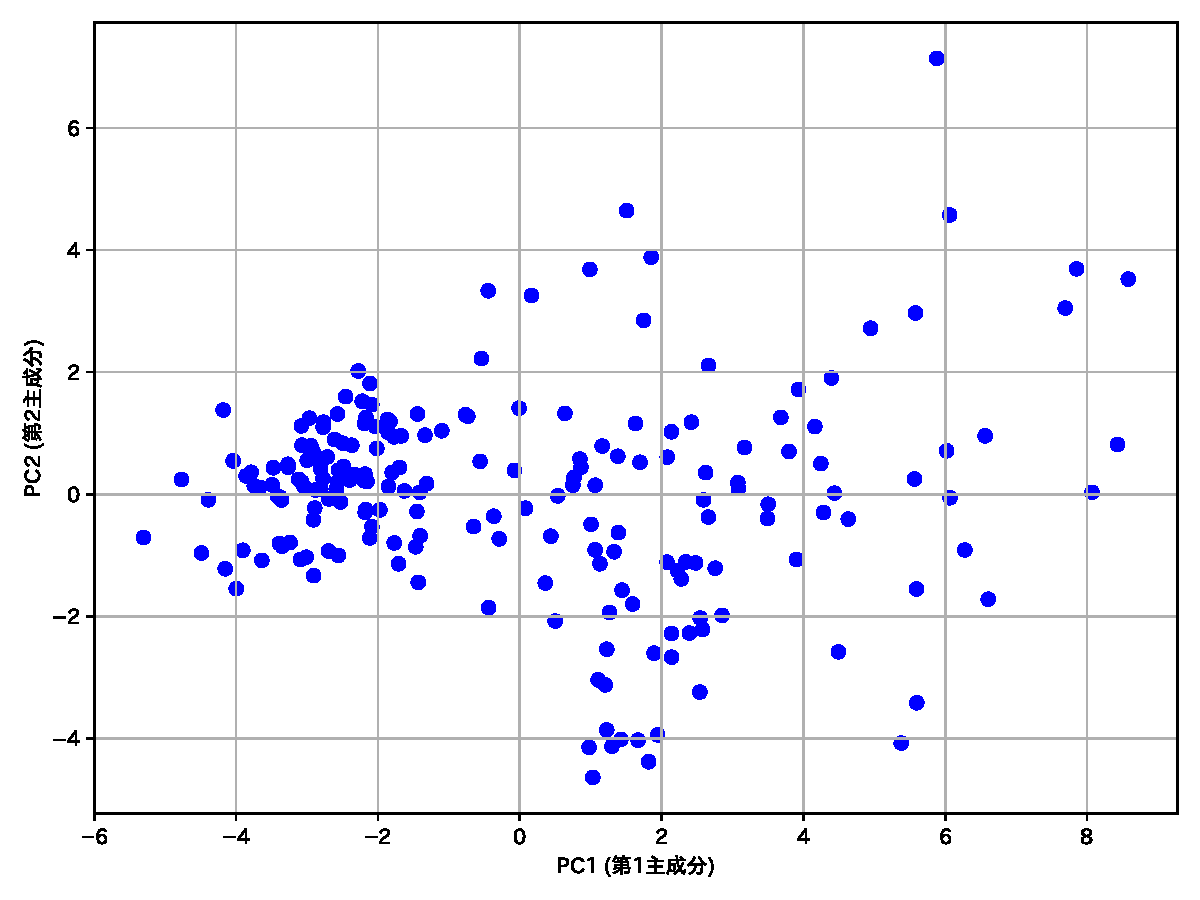
\includegraphics[width=1.0\linewidth]{Okamoto_fig/pca-10.pdf}
	\caption{ユーザのCT獲得過程パターン(10作品制作したユーザ)}
 \ecaption{Patterns of CT Proficiency Processes for Users Who Created 10 Works}
	\label{fig:pca}
 \vspace{-2mm}
\end{figure}

\textcolor{red}{
[変更2-1-c,変更2-3]本研究では,ユーザのCTスコア獲得過程のパターンによる違いを調査するため,事前分析を行う.具体的には,従来研究\cite{Ando_2021}で用いられていたデータセットのユーザから,{$N~(3 \leq N \leq 20)$}個の作品を制作した各ユーザのCTスコア獲得過程を($N \times 7$)次元のベクトルとして平坦化し,主成分分析を行う.図\ref{fig:pca}は,11作品目にDevelopingまたはMasterの作品を制作したユーザが習熟度が向上するまでの10作品分のCT獲得過程パターンを散布図を示す.第1主成分,第2主成分の固有値はそれぞれ2.9,9.8であり1以上であるため,データを十分に説明できていると考える.その上で,散布図の全体的にばらつきが見られ,CT獲得過程のパターンがユーザによって異なることを明らかにしました.他の制作回数を持つユーザにおいても同様の傾向が見られ,CTスコア獲得過程におけるパターンの多様性を確認した.このように,ユーザによって作品の制作過程で使用されるCTスキルが異なるため,本研究では,ユーザの作品制作過程で使用されるCTスキル,および各CTスキルを用いた作品制作数を明らかにし,CT概念の習熟過程やCTスキルの成長パターンの理解を研究の狙いとする.
}

% 本研究では事前分析として,ユーザが初めてDeveloping以上またはMasterに到達した作品のCTスキルを調査する.表\ref{tab:ranking-btod},表\ref{tab:ranking-dtom}は,紙面の都合上,同じ概念を使用して制作した作品数の多いそれぞれ3パターンのみを示す.Developingに到達する作品の中で,並列,同期の点数が異なる.また,Masterに到達した作品は合計点数の分散がDevelopingに到達する作品に比べて大きく,抽象化,同期,フロー制御の点数が異なる.このように,特定の習熟度に到達した作品の中でも使用されるCTスキルが異なるため,それまでに制作した作品に使用したCTスキルも異なることが示唆される.本研究では,特定の習熟度に到達するまでの過程で使用されるCTスキル,および各CTスキルを用いた作品制作数を明らかにし,CT概念の習熟過程やCTスキルの成長パターンの理解を研究の狙いとする.


% 安東ら~\cite{Ando_2021}はユーザのCTに合わせた作品推薦に向けて,ユーザが過去に制作した作品のCTスキルに基づいてユーザが次にCT習熟度が向上するかを予測する研究を行なった.事前分析としてユーザがScratch上に公開している作品を収集し,各作品で使用されるCT概念をDr.Scratchを用いて計測し,ユーザが特定の習熟度に到達するまでに制作した作品の特徴を分析した.分析結果として,ユーザにとって習熟度DevelopingやMasterに分類されるオリジナル作品の制作は困難であり,ユーザは類似するCTスコアの作品を連続して制作することで習熟度が向上することが示唆された.特に,習熟度Developingのオリジナル作品を制作するまでに,ユーザは連続してBasicやDevelopingの作品を制作することが多く,Masterの作品を制作することは少ないことがわかり,習熟度Masterのオリジナル作品を制作するユーザの数は少なく,Masterの作品を連続して制作することは少ないことがわかった.また,ユーザが過去に使用したCT概念に基づき,ユーザが次に制作する作品が当該習熟度以上の評価を得るかを予測するモデルとして,事前分析の結果に基づき,目的変数の異なる2種類のモデルを構築した.

% \begin{description}
% \item [モデル1:]習熟度がDeveloping以上のオリジナル作品を制作するユーザを予測
% \item [モデル2:]習熟度がMasterのオリジナル作品を制作するユーザを予測
% \end{description}

% 説明変数としてはユーザが過去に作品制作で使用した7つのCT概念の0点から3点の獲得有無を用いた.モデルの構築にはランダムフォレストを用いており,事前分析で収集したデータを基に構築,予測を行った.結果としてDevelopingやMasterに到達するユーザと到達しないユーザの間では,過去に使用したCT概念に違いがあることが示唆された.

% 多くの従来研究では,Scratch上でユーザが制作する作品の特徴,またはCTスキル習熟過程全体で使用するCT概念を調査しており,一部のCT概念の学習が困難であること,また特定の習熟度に到達するユーザとそうでないユーザ間では獲得したCT概念に違いがあることを明らかにしている.しかし,従来研究ではCT7概念の詳細な獲得過程の特徴については明らかになっていない.

% 表\ref{tab:same-path}は安東らが行なった従来研究\cite{Ando_2021}の対象ユーザのうち,CTパス:ユーザが獲得してきたCT7概念が同じだったユーザのペア数と従来モデルの予測結果が異なるペア数,予測がどちらも外れたペア数を示す.表\ref{tab:same-path}のモデル1では,予測がどちらも外れたペア数が512と多く,予測結果が異なるペア数と予測がどちらも外れたペア数を合わせるとCTパスが同じ全てのペアのうち,約13\%が予測が異なる,あるいは予測が外れていることがわかる.また,表\ref{tab:same-path}のモデル2では予測結果が異なるペア数と予測がどちらも外れたペア数のどちらも数は小さいものの,CTパスが同じ全てのペア数のうち,約30\%を占めていることがわかる.このことから,従来モデルではユーザのCT概念の獲得有無のみを説明変数としているため,ユーザのCT概念獲得過程は考慮されていないことが考えられる.しかし,実際にユーザは習熟度が向上するまでに様々なCTスキル習熟過程があることを確認している.

% したがって,ユーザのCT7概念の獲得過程に基づいて,当該ユーザが保有するCTの習熟度の特定ができれば,ScratchにおけるユーザのCTスキル獲得状況に合わせた学習の参考となる作品提示等の学習支援の役立てとなると期待する.

% \begin{table}
%   \caption{同じCTパスを持つユーザのペア数}
%   \label{tab:same-path}
%   \vspace{2mm}
%   \centering
%   \begin{tabular}{c|c|c|c}
%     \hline
%      &  \begin{tabular}[c]{@{}c@{}}予測結果が\\異なるペア数\end{tabular} & \begin{tabular}[c]{@{}c@{}}予測がどちらも\\外れたペア数\end{tabular} & 全てのペア数\\
%     \hline
%     \hline
%     モデル1 & 24 & 512 & 4,094 \\
%     \hline
%     モデル2 & 14 & 5 & 63 \\
%     \hline
%   \end{tabular}
% \end{table}


%%%%%%%%%%%%%%%%%%%%%%
\section{データセット}\label{sec:chapter_3-1}
%%%%%%%%%%%%%%%%%%%%%%
本研究では,従来研究~\cite{Ando_2021}と同様に,2019年1月3日から2020年1月3日までの間に初めて作品公開を行い,分析対象期間中に20件以上の作品を制作し,且つ全ての作品でDr.ScratchでCTスコアの計測が成功したユーザ6,323人(各人20作品,合計126,460作品)を分析対象とする.本研究では,ユーザが一度でも特定の習熟度を満たす作品を制作すれば当該習熟度に到達したと判断し,リミックスによって制作された作品は習熟度に到達したと判断しない.分析対象のユーザの中で,20番目の作品を制作するまでにBasicからDeveloping以上に向上したユーザ(BtoDユーザ)3,125人,DevelopingからMasterに向上したユーザ(DtoMユーザ)1,196人を確認した.また,20作品を制作する過程で,BasicからDevelopingに向上し,さらにDevelopingからMasterに向上するユーザもいるため,BtoDユーザとDtoMユーザの間には重複がある.

%---------------------
\begin{figure}[t]
    \centering
    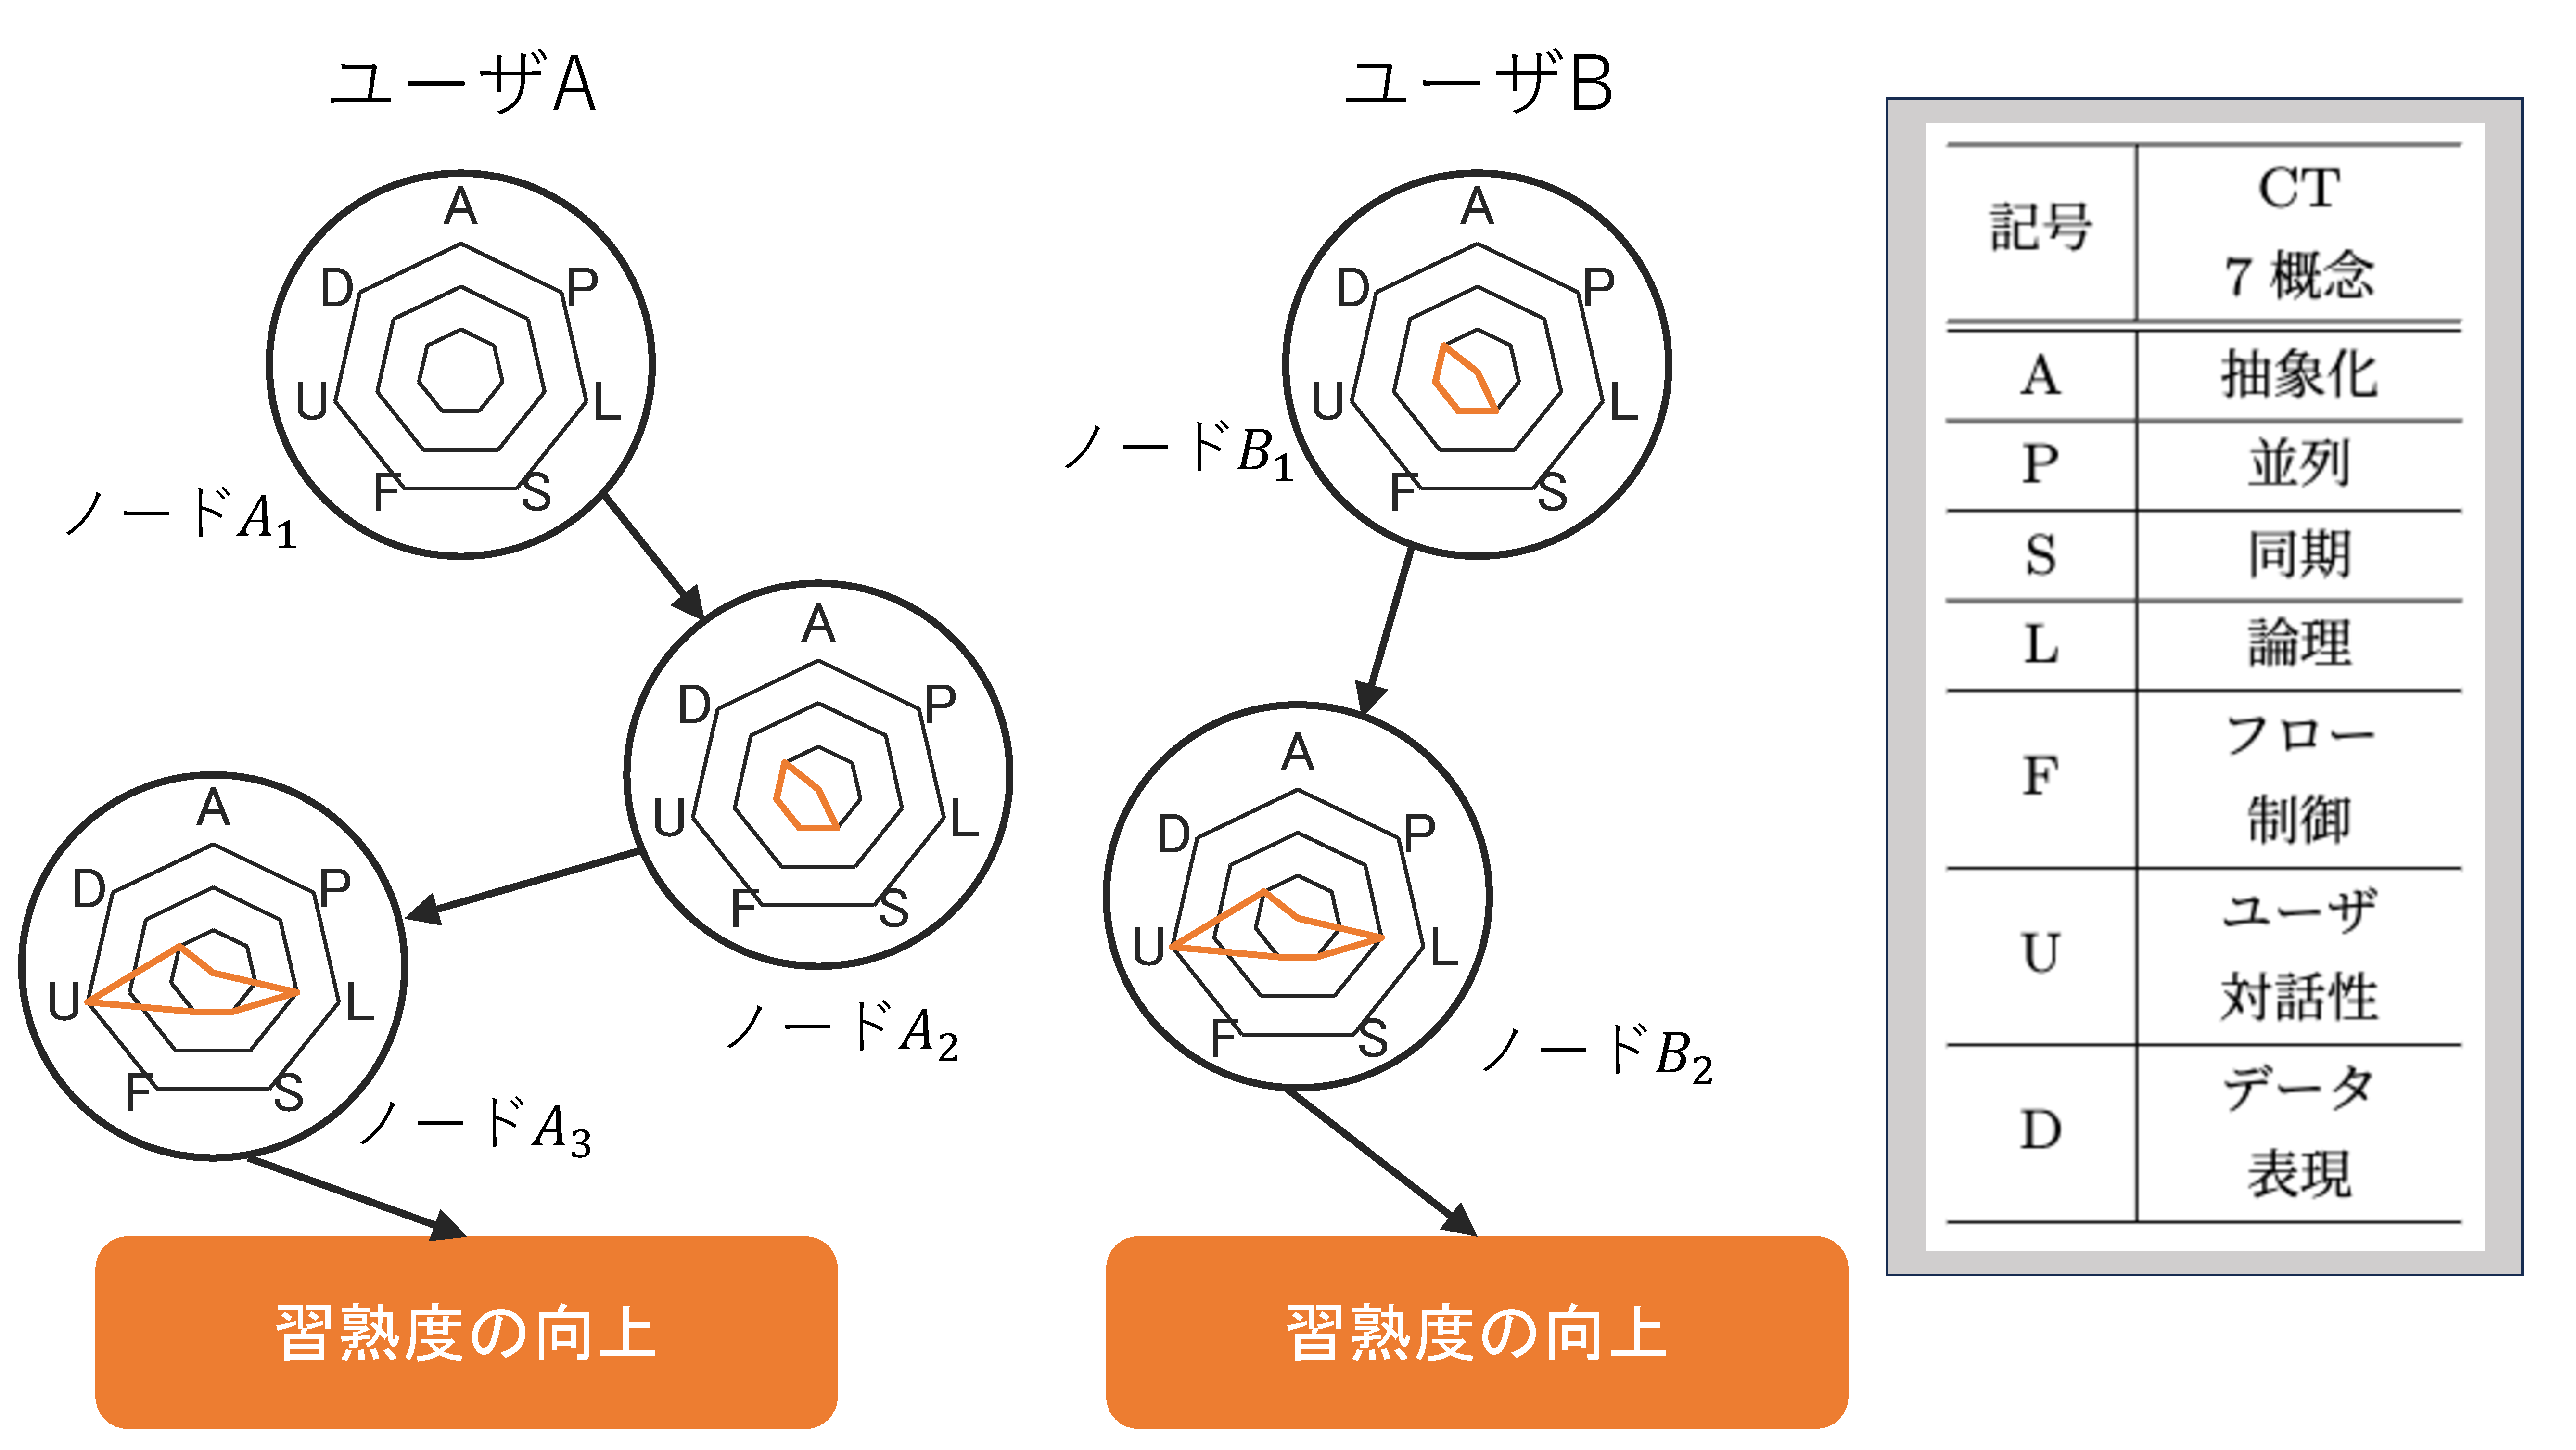
\includegraphics[width=1.0\linewidth]{Okamoto_fig/graph.pdf}
    \caption{BtoDユーザ2人のCTパス事例}
    \ecaption{Example of CT paths for 2 BtoD users}
    \label{fig:digraph}
    \vspace{-4mm}
\end{figure}
%---------------------

%%%%%%%%%%%%%%%%%%%%%%
\section{RQ1:CT習熟度が向上するユーザが\textcolor{red}{[変更2-2]共通して}過去の作品で使用するCTスキルの特徴は?}\label{sec:chapter_3-2}
%%%%%%%%%%%%%%%%%%%%%%
\subsection{分析手法}\label{sec:rq1-approach}

% 従来研究ではユーザが一度でも特定の習熟度を満たす作品を制作すれば当該習熟度に到達したと判断しており,リミックス作品による獲得は習熟度到達として認めていない.本研究では,従来研究の設定と同様に,20番目の作品を制作するまでにBasicからDeveloping以上に向上したユーザ(BtoDユーザ)3,125人,DevelopingからMasterに向上したユーザ(DtoMユーザ)1,196人を分析対象とする.また,20番目の作品を制作する過程で,BasicからDevelopingに向上し,さらにDevelopingからMasterに向上するユーザもいるため,BtoDユーザとDtoMユーザの間には重複がある.
\textcolor{red}{[変更2-7-a]
従来研究\cite{Ando_2021}において,BtoDユーザとDtoMユーザ間で習熟度が向上するまでに制作する作品のCT概念の特徴は異なることが明らかとなった.そのため,本研究では,BtoDユーザ,DtoMユーザそれぞれで習熟度が向上するまでに制作した作品で使用したCTスコアの系列(CTパス)を追跡する.
}
%BtoDユーザとDtoMユーザそれぞれについて,習熟度が向上するまでに獲得したCT7概念の系列(CTパス)を抽出し,\todo{抽出して何する?}する.リミックス作品も学習の一部とみなし,習熟度向上の過程で制作されたリミックス作品もCTパスに含める.
図\ref{fig:digraph}は2人のBtoDユーザのCTパスの概略図を示す.ユーザAはDevelopingの作品を制作するまでに3作品($A_1$,$A_2$,$A_3$),ユーザBは2作品($B_1$,$B_2$)を制作している.図中には各作品をノードで表現し,ノード内のレーダーチャートは,CT概念7種類のスコアを示す.レーダーチャートの最外側がCTスコア3点,最内側がCTスコア0点とする.ノード間のエッジはユーザによる作品の制作順序を表す.ユーザAの最初の作品($A_1$)は,全てのCTスコアが0点,2番目の作品($A_2$)はフロー制御,ユーザ対話性,データ表現の概念を1点を獲得している.3番目の作品($A_3$)ではユーザ対話性と論理の概念で\textcolor{red}{\UnderlineTex{[変更1-2-1]3}}点を獲得し,4番目で習熟度Developingに到達している.過去の作品でリミックス作品を制作した場合も,ユーザにとっては学習の一部とみなし,習熟過程で制作されたリミックス作品はCTパスに含める.

% 図中のノードは,制作された作品から測定されたCT7概念のスコア分布を示し,次に制作する作品へのつながりはエッジで表現する.各ノード内のレーダーチャートのラベル記号は,対応するCT7概念に一致し,表\ref{tab:ct-symobol}にその対応関係を示す.各項目はチャートの最外側が3点,最内側が0点とする.図\ref{fig:digraph}のBtoDユーザAは最初に全てのCTスコアが0点の作品を制作し,次にフロー制御,ユーザ対話性,データ表現の概念を1点を獲得した後,ユーザ対話性と論理の概念で2点向上させ,習熟度Developingに到達している.リミックス作品も学習の一部とみなし,習熟度向上の過程で制作されたリミックス作品もCTパスに含める.

\textcolor{red}{[変更1-2-2]\UnderlineTex{RQ1では,多くのユーザが制作する作品の特徴を明らかにするため,各ユーザがCT習熟度が向上するまでに制作した作品数と,BtoDユーザ,DtoMユーザ毎の隣接するノード間のエッジの重複数(CTパス重複数)を算出する.例えば,図1のノード$A_1$とノード$B_1$,ノード$A_2$とノード$B_2$で制作された作品は同じCT概念を用いているため,CTパスが重複しており,CTパス重複数は2となる.ユーザのCTパス全体の再現性を確認するため,ユーザのCTパスの各CTパス重複数を合計し,エッジ数で割った平均値を用いて,より数値の高いCTパスを持つユーザを抽出する.本手法により特定の習熟度に到達するまでの過程で使用されるCTスキルの特徴を明らかにできる.}}

% RQ1では,特定の習熟度に到達するまでの過程で使用したCTスキル,および各CTスキルを用いたユーザの作品制作数を分析し,多くのユーザが制作する作品の特徴を明らかにする.具体的には,特定の習熟度に到達するまでに,多くのユーザが共通して使用するCTスキルを追跡する.図\ref{fig:digraph}の例では,2人のユーザが特定の習熟度に到達するまでにノード$A_2$とノード$B_1$,ノード$A_3$とノード$B_2$の作品でCTスキルが共通していることがわかる.本手法により特定の習熟度に到達するまでの過程で使用されるCTスキルの特徴を明らかにできる.

% のユーザAは習熟度が向上するまでに制作した作品数が3であり,ユーザBは2である.また,ノード$A_1$とノード$B_1$,ノード$A_2$とノード$B_2$で制作された作品は同じCT概念を用いているため,CTパスが重複している.ユーザのCTスキル習熟過程の再現性を確認するため,ユーザのCTパス重複数として,ユーザのCTパスの各エッジの重複数を合計し,エッジ数で割った平均値を用いる.ユーザAとユーザBのみを分析する場合,ユーザAの各エッジの重複数は1,2,2となり,ユーザAのCTパス重複数は$(1 + 2 + 2) / 3 = 1.67$となる.

RQ1では,多くのユーザが制作する作品の特徴を明らかにするため,各ユーザがCT習熟度が向上するまでに制作した作品数と,BtoDユーザ,DtoMユーザ毎の隣接するノード間のエッジの重複数(CTパス重複数)を算出する.例えば,図\ref{fig:digraph}のノード$A_1$とノード$B_1$,ノード$A_2$とノード$B_2$で制作された作品は同じCT概念を用いているため,CTパスが重複していると言え,CTパス重複数は2となる.ユーザのCTパス全体の再現性を確認するため,ユーザのCTパスの各CTパス重複数を合計し,エッジ数で割った平均値を用いて,より数値の高いCTパスを持つユーザを抽出する.本手法により特定の習熟度に到達するまでの過程で使用されるCTスキルの特徴を明らかにできる.


% 本分析では,より特徴のあるCTパスを抽出するため,習熟度を向上させる際に制作した作品のCT概念の重複数が多いユーザに着目する.また,ユーザが習熟度向上までにかかる作品数による違いも明らかにするため,習熟度向上までに制作した作品数毎のCTパス(代表CTパス)を抽出する.代表CTパスは習熟度向上までに制作した作品数毎に取得したCTパスに対し,以下の操作を行なって抽出する.
% \begin{enumerate}
%     \item 習熟度向上までに制作した作品数毎に各エッジの重複数を算出する.
%     \item 習熟度向上の際に作成した作品から最大のエッジの重複数を持つノードに移る.
%     \item 現在のノードの直前にある最大のエッジの重複数を持つノードを確認する.
%     \item 最大のエッジの重複数を持つノードが一つしか存在しなかった場合そのノードに移り,3の操作を行う.複数ある場合は5の操作を行う.現在のノードが初期ノードである場合,6の操作を行う.
%     \item ユーザ全体のCTパスから各エッジの重複数(重要度)を算出し,4で特定した複数のエッジの中から,重要度が最も高いエッジの重複数を持つノードに移り,3の操作を行う.現在のノードが初期ノードである場合,6の操作を行う.
%     \item 現在のノードまでに辿ってきたパスを代表CTパスとして抽出する.
% \end{enumerate}



%---------------------
% \begin{table}[t]
%   \caption{記号とCT7概念の対応表}
%   \label{tab:ct-symobol}
%   \vspace{2mm}
%   \centering
%   \begin{tabular}{c|c}
%     \hline
%     記号 & \begin{tabular}{c}CT\\7概念\end{tabular}\\
%     \hline
%     \hline
%     A & 抽象化 \\
%     \hline
%     P & 並列 \\
%     \hline
%     S & 同期 \\
%     \hline
%     L & 論理 \\
%     \hline
%     F & \begin{tabular}{c}フロー\\制御\end{tabular} \\
%     \hline
%     U & \begin{tabular}{c}ユーザ\\対話性\end{tabular} \\
%     \hline
%     D & \begin{tabular}{c}データ\\表現\end{tabular} \\
%     \hline
%   \end{tabular}
% \end{table}
%---------------------


\vspace{-2mm}
\subsection{分析結果}\label{sec:3-analysis}

\subsubsection{ユーザが使用するCTスキルの共通性の分析}\label{subsec:path-analysis}

本分析では,複数のユーザが共通のCTスキルを使用して制作した作品数(重複数)を分析することで,多くのユーザが特定の習熟度に到達するまでに使用したCT概念や制作した作品数などのCT概念の習熟過程を明らかにすることができる.%従来研究\cite{Ando_2021}においてユーザが特定の習熟度に到達するまでに共通のCTを使用することが明らかにされている.
%特定の習熟度に到達するためにCTを習得することが必要であるとは限らないが,習得することで学習を効率化できることが示唆される.
図\ref{fig:digraph}の例を用いて,\textcolor{red}{\UnderlineTex{[変更1-2-2]CTパス}}重複数の算出方法を説明する.ユーザAは制作した3つの作品のうち,$A_1$はユーザBのいずれの作品ともCTスキルが共通していないため重複数は1,$A_2$は$B_1$と共通のCTスキルを使用しているため重複数は2,$A_3$は$B_2$と共通のCTスキルを使用しているため重複数は2となり,ユーザAが制作した作品の\textcolor{red}{\UnderlineTex{[変更1-2-2]CTパス}}平均重複数は1.67 ($=(1 + 2 + 2) / 3$)となる.

図\ref{fig:dupli-mean}は,全てのユーザの\textcolor{red}{\UnderlineTex{[変更1-2-2]CTパス}}平均重複数を習熟度別に算出した分布を箱ひげ図で示す.BtoDユーザとDtoMユーザの\textcolor{red}{\UnderlineTex{[変更1-2-2]CTパス}}平均重複数は,それぞれ中央値が10.5(平均値35.8),中央値が1.0(平均値2.4)であった.Mann-Whitney U検定(p値$<$0.05)を適用した結果,BtoDユーザとDtoMユーザの\textcolor{red}{\UnderlineTex{[変更1-2-2]CTパス}}平均重複数に統計的有意差が見られた.したがって,BtoDユーザがDeveloping以上に到達するまでに制作した作品は,共通して使用するCTスキルが存在すると示唆される.

% 再現性のあるCTパスをたどって習熟度を向上させていることがわかる.一方,DtoMユーザのCTパスの重複数は,中央値が1.0,平均値が2.4となっており,DevelopingからMasterレベルに習熟度を向上させるユーザは,より多様なCTパスを経由して習熟度を向上させていることが示されている.BtoDユーザとDtoMユーザ間でMann-Whitney U検定\cite{Mann1947OnAT}を適用した結果,統計的に有意差(p値$<$0.05)が確認されたことから,BtoDユーザとDtoMユーザが異なるCTパスを辿って習熟度を向上させていることを示している.

% また,図\ref{fig:path-length}は各習熟度レベルに向上するまでにユーザが制作する作品数の分布を示す箱ひげ図である.BtoDユーザが習熟度を向上させるまでに制作する作品数の中央値は6.0,平均値は7.2であり,DtoMユーザのそれは中央値が10.0,平均値が9.6であった.BtoDユーザとDtoMユーザ間でMann-Whitney U検定を実施したところ,統計的に有意な差(p値$<$0.05)が見られたことから,習熟度を向上させる過程で必要とする作品数にはグループ間で差があり,BtoDユーザはDtoMユーザに比べてより短期間で特定の習熟度に到達している.
%---------------------
\begin{figure}[t]
	\centering
	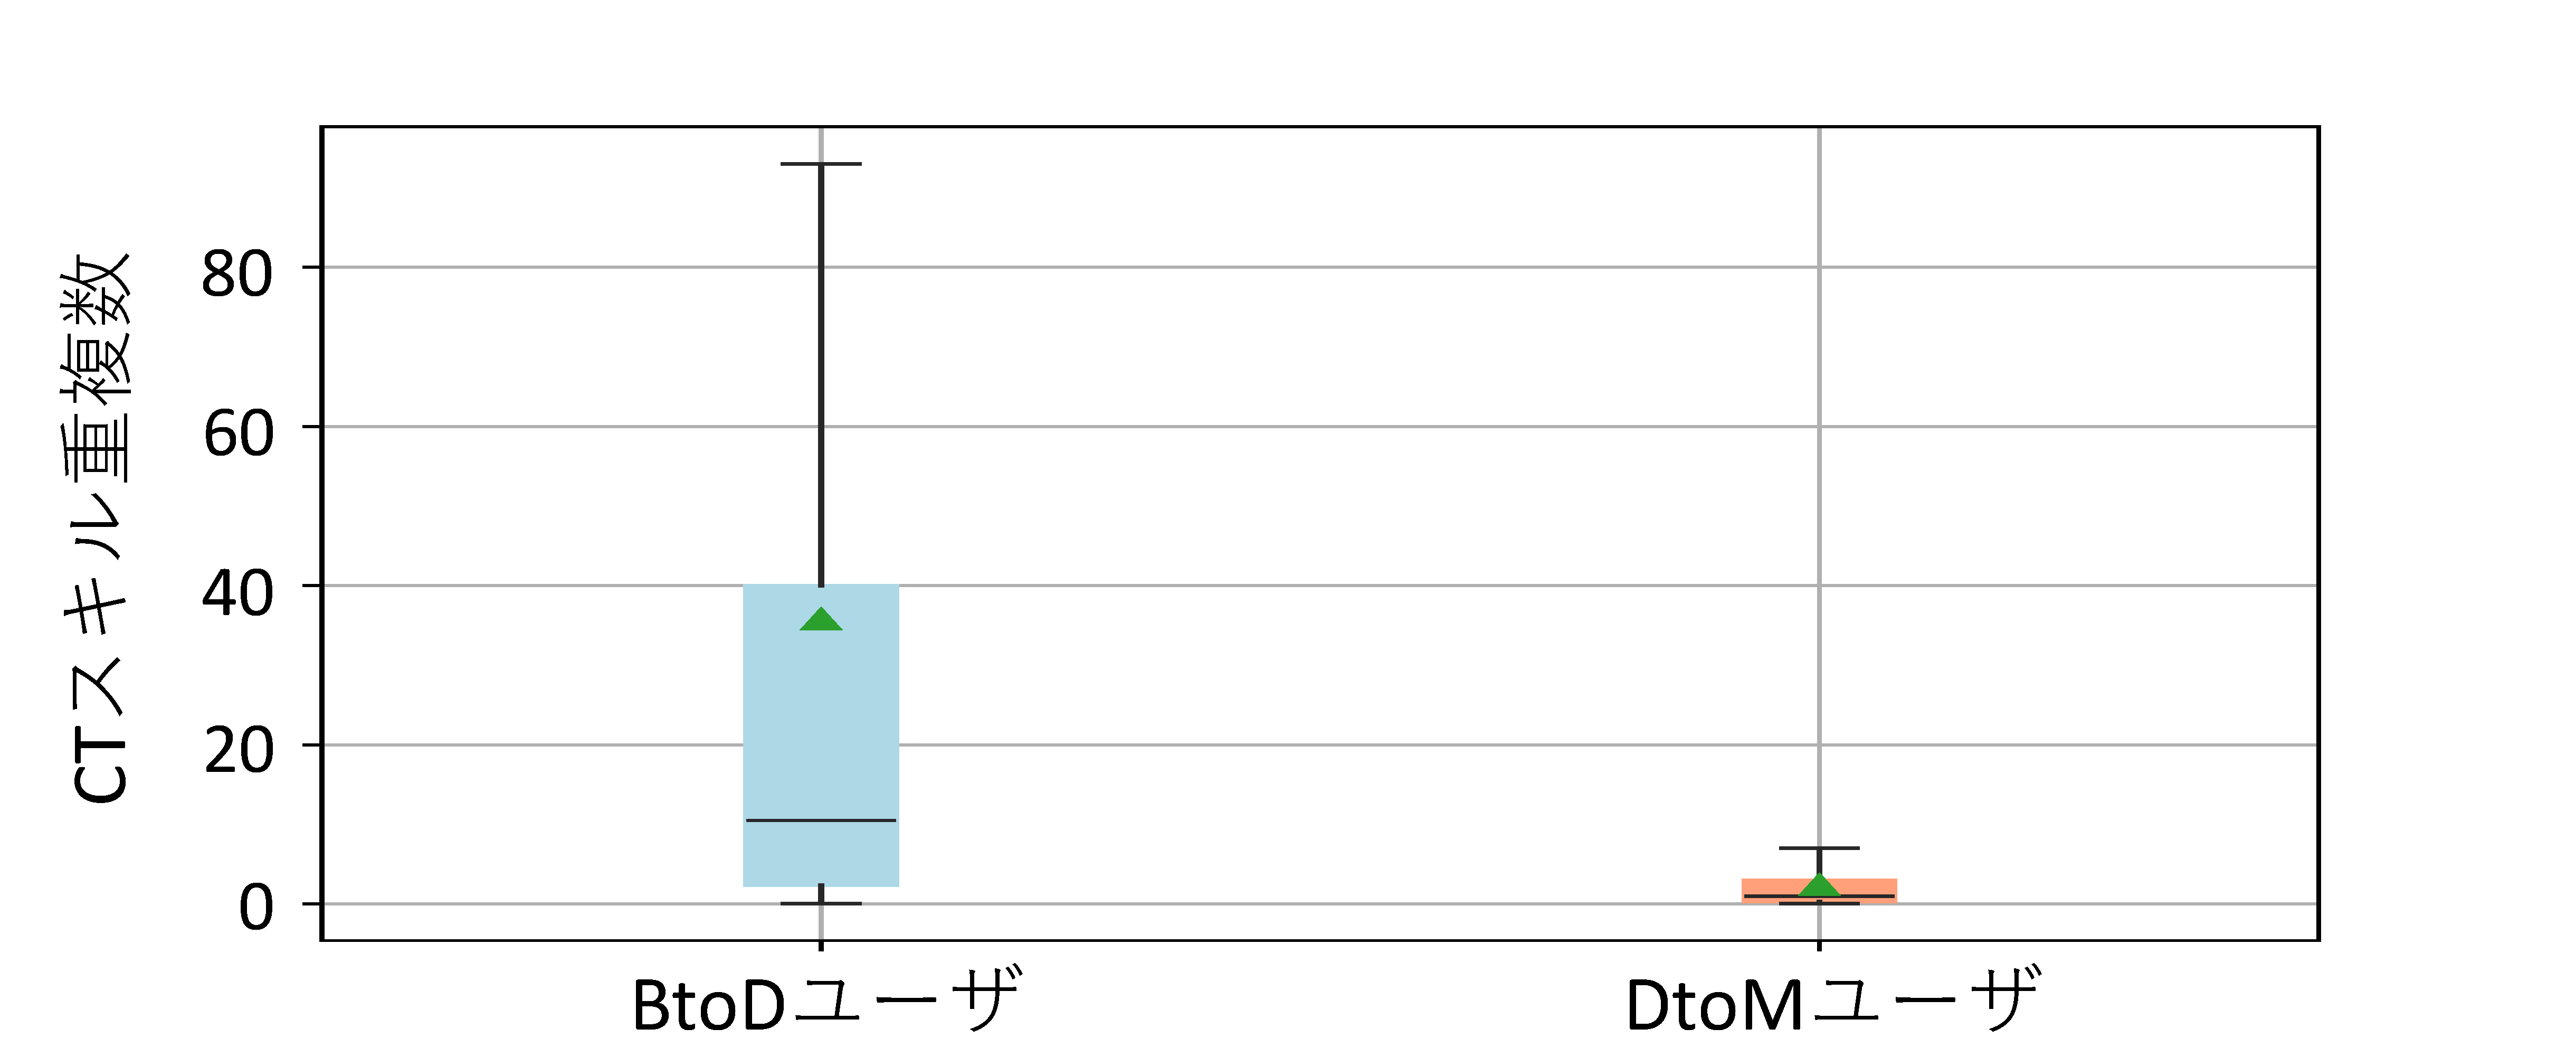
\includegraphics[width=0.8\linewidth]{Okamoto_fig/dupli-all.pdf}
	\caption{各習熟度に到達したユーザの\textcolor{red}{\UnderlineTex{[変更1-2-2]CTパス}}平均重複数の分布}
        \ecaption{Distribution of the number of CT skill overlaps for each BtoD users and DtoM users.}
	\label{fig:dupli-mean}
 \vspace{-2mm}
\end{figure}

%\begin{figure}[t]
% 	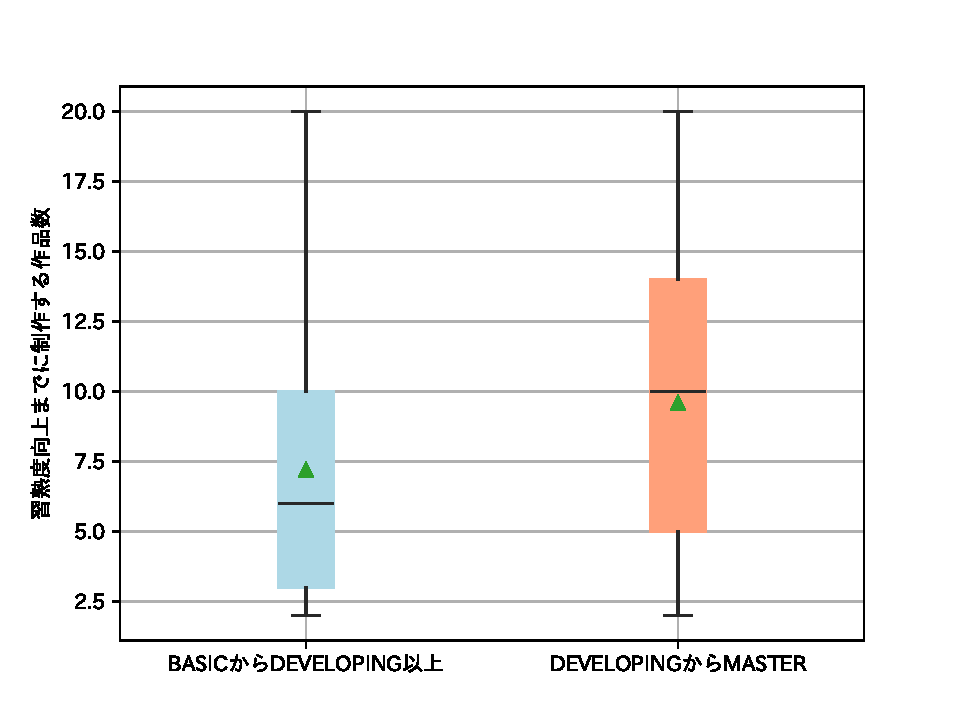
\includegraphics[width=1.0\linewidth]{Okamoto_fig/path-length.pdf}
%         \vspace{-5mm}
% 	\caption{各習熟度に到達したユーザが習熟度向上までに制作する作品数の分布}
% 	\label{fig:path-length}
% \end{figure}
% %---------------------

\subsubsection{制作過程で使用するCTスキルの分析}\label{subsec:ct-analysis}

% 表\ref{tab:ranking-btod}にBtoDユーザの中で,習熟度を向上させる際に制作した作品のCT概念の重複数が上位10件にランクされたユーザを示す.CT概念に用いている記号は\ref{sec:chapter_3-2}節で用いた表\ref{tab:ct-symobol}と対応している.データセットから抽出した全BtoDユーザ3,125人の中で,表\ref{tab:ranking-btod}に示す上位10件のCT概念を使用する作品制作したユーザ数は1,209人(約39\%)である.この1,209人の各CT概念において,全ユーザが抽象化で1点を獲得しており,8位を除く全てでデータ表現のスキルを1点獲得している.つまり,多くのBtoDユーザが最終的に抽象化とデータ表現のスキルを獲得していることを示している.



% 表\ref{tab:ranking-dtom}にDtoMユーザの中で,習熟度を向上させる際に制作した作品のCT概念の重複数が上位10件にランクされたユーザを示す.CT概念に用いている記号は\ref{sec:chapter_3-2}節で用いた表\ref{tab:ct-symobol}と対応している.データセットから抽出した全DtoMユーザ1,196人の中で,表\ref{tab:ranking-dtom}に示す上位10件のCT概念を使用する作品制作したユーザ数は523人(約44\%)であった.この523人の各CT概念において,全ユーザがユーザ対話性とデータ表現のスキルで2点を獲得しており,10位を除く全てで並列処理のスキルを3点獲得している.これは,多くのDtoMユーザが最終的にユーザ対話性,データ表現,並列処理のスキルを獲得していることを示している.



%-----------------------
\begin{table*}[t]
  \begin{minipage}[t]{0.45\linewidth} % 0.5\linewidthはページ幅の半分に相当
    \centering
    \caption{BtoDユーザが習熟度向上までに制作した\\作品数毎の代表CTパス}
    \ecaption{Representative CT paths for each number of\\works produced by BtoD users.}
    \label{tab:split-ct-btod}
    \vspace{1mm}
      \scalebox{0.85}{ 
  \begin{tabular}{c|l|r}
    \hline\hline
    作品数 & 代表CTパス & \multicolumn{1}{c}{ユーザの割合}\\
    \hline
    1 & \texttt{\large{A}} & 17\%(10/58) \\
    \hline
    2 & \texttt{\large{\textcolor{Green}{BB}}} & 43\%(18/42) \\
    \hline
    3 & \texttt{\large{\textcolor{Green}{BBB}}} & \textcolor{red}{\UnderlineTex{[変更1-3-13]39}}\%(13/33) \\
    \hline
    4 & \texttt{\large{ACDE}} & 28\%(9/32) \\
    \hline
    5 & \texttt{\large{\textcolor{Green}{F}GH\textcolor{Green}{F}I}} & 33\%(6/18) \\
    \hline
    6 & \texttt{\large{J\textcolor{Green}{B}KLJM}} & 20\%(2/10) \\
    \hline
    7 & \texttt{\large{\textcolor{Green}{FFFFFFF}}} & 35\%(6/17)  \\
    \hline
    8 & \texttt{\large{JJJJJJJM}} & 40\%(4/10) \\
    \hline
    9 & \texttt{\large{\textcolor{blue}{NNN}H\textcolor{Green}{B}KH\textcolor{Green}{J}M}} & 17\%(2/12) \\
    \hline
    10 & \texttt{\large{\textcolor{Green}{BBBBBBBBB}O}} & 29\%(2/7) \\
    \hline
    11 & \texttt{\large{\textcolor{blue}{NNNNNNNN}P\textcolor{Green}{B}I}} & 33\%(1/3) \\
    \hline
    12 & \texttt{\large{\textcolor{blue}{NNNNNNNNNNNN}}} & 27\%(3/11) \\
    \hline
    13 & \texttt{\large{\textcolor{blue}{LLLLLLLLLLLQ}R}} & 50\%(2/4) \\
    \hline
    14 & \texttt{\large{N\textcolor{Green}{B}S\textcolor{blue}{N}\textcolor{Green}{B}S\textcolor{blue}{N}\textcolor{Green}{B}S\textcolor{blue}{N}\textcolor{Green}{B}S\textcolor{blue}{N}\textcolor{Green}{B}}} & 50\%(2/4) \\
    \hline
    15 & \texttt{\large{\textcolor{blue}{QQQQQQQQQQQQQQ}T}} & 25\%(4/16) \\
    \hline
    16 & \texttt{\large{UO\textcolor{blue}{Q}VWUO\textcolor{blue}{Q}VWUO\textcolor{blue}{Q}VX\textcolor{Green}{B}}} & 33\%(1/3) \\
    \hline
    17 & \texttt{\large{CYACYACYACYACYACZ}} & 50\%(2/4) \\
    \hline
    18 & \textcolor{blue}{\texttt{\large{NNNNNNNNNNNNNNNNNN}}} & 40\%(2/5) \\
    \hline
  \end{tabular}
  }
  \end{minipage}%
  \begin{minipage}[t]{0.5\linewidth}
    \centering
    \caption{BtoDユーザの制作作品を対象とした代表CTパスの記号とCT概念の対応表}
    \ecaption{CT concept and the score in symbol of the representative\\CT path for BtoD users.}
    \label{tab:dict-btod}
    \vspace{7mm}
      \scalebox{0.85}{ 
      \begin{tabular}{c|c|cccccccc}
\hline\hline
\multirow{2}{*}{記号} & \multicolumn{1}{l|}{\multirow{2}{*}{\small{リミックス}}} & \multicolumn{8}{c}{CTスコア}  \\ \cline{3-10} 
                    & \multicolumn{1}{l|}{}                       & \multicolumn{1}{c|}{A} & \multicolumn{1}{c|}{P} & \multicolumn{1}{c|}{L} & \multicolumn{1}{c|}{S} & \multicolumn{1}{c|}{F} & \multicolumn{1}{c|}{U} & \multicolumn{1}{c|}{D} & 合計 \\ \hline 
\texttt{\large{A}}                   & 0                                           & \multicolumn{1}{c|}{0} & \multicolumn{1}{c|}{0} & \multicolumn{1}{c|}{0} & \multicolumn{1}{c|}{0} & \multicolumn{1}{c|}{1} & \multicolumn{1}{c|}{1} & \multicolumn{1}{c|}{1} & 3  \\ \hline
\rowcolor{Green!30}%
\texttt{\large{B}}                   & 0                                           & \multicolumn{1}{c|}{1} & \multicolumn{1}{c|}{1} & \multicolumn{1}{c|}{0} & \multicolumn{1}{c|}{1} & \multicolumn{1}{c|}{2} & \multicolumn{1}{c|}{1} & \multicolumn{1}{c|}{1} & 7  \\ \hline
\texttt{\large{C}}                   & 0                                           & \multicolumn{1}{c|}{0} & \multicolumn{1}{c|}{0} & \multicolumn{1}{c|}{0} & \multicolumn{1}{c|}{0} & \multicolumn{1}{c|}{0} & \multicolumn{1}{c|}{0} & \multicolumn{1}{c|}{0} & 0  \\ \hline
\rowcolor{Green!30}%
\texttt{\large{F}}                   & 0                                           & \multicolumn{1}{c|}{1} & \multicolumn{1}{c|}{1} & \multicolumn{1}{c|}{0} & \multicolumn{1}{c|}{0} & \multicolumn{1}{c|}{2} & \multicolumn{1}{c|}{1} & \multicolumn{1}{c|}{1} & 6  \\ \hline
\texttt{\large{J}}                   & 0                                           & \multicolumn{1}{c|}{0} & \multicolumn{1}{c|}{0} & \multicolumn{1}{c|}{0} & \multicolumn{1}{c|}{0} & \multicolumn{1}{c|}{2} & \multicolumn{1}{c|}{2} & \multicolumn{1}{c|}{1} & 5  \\ \hline
\rowcolor{blue!30}%
\texttt{\large{L}}                   & 0                                           & \multicolumn{1}{c|}{0} & \multicolumn{1}{c|}{0} & \multicolumn{1}{c|}{0} & \multicolumn{1}{c|}{1} & \multicolumn{1}{c|}{1} & \multicolumn{1}{c|}{2} & \multicolumn{1}{c|}{1} & 5  \\ \hline
\rowcolor{blue!30}%
\texttt{\large{N}}                   & 0                                           & \multicolumn{1}{c|}{0} & \multicolumn{1}{c|}{0} & \multicolumn{1}{c|}{0} & \multicolumn{1}{c|}{0} & \multicolumn{1}{c|}{2} & \multicolumn{1}{c|}{1} & \multicolumn{1}{c|}{1} & 4  \\ \hline
\texttt{\large{O}}                   & 0                                           & \multicolumn{1}{c|}{1} & \multicolumn{1}{c|}{1} & \multicolumn{1}{c|}{0} & \multicolumn{1}{c|}{1} & \multicolumn{1}{c|}{1} & \multicolumn{1}{c|}{1} & \multicolumn{1}{c|}{1} & 6  \\ \hline
\rowcolor{blue!30}%
\texttt{\large{Q}}                   & 0                                           & \multicolumn{1}{c|}{1} & \multicolumn{1}{c|}{0} & \multicolumn{1}{c|}{0} & \multicolumn{1}{c|}{0} & \multicolumn{1}{c|}{1} & \multicolumn{1}{c|}{2} & \multicolumn{1}{c|}{1} & 5  \\ \hline
\texttt{\large{S}}                   & 0                                           & \multicolumn{1}{c|}{1} & \multicolumn{1}{c|}{0} & \multicolumn{1}{c|}{0} & \multicolumn{1}{c|}{1} & \multicolumn{1}{c|}{1} & \multicolumn{1}{c|}{2} & \multicolumn{1}{c|}{1} & 6  \\ \hline
\texttt{\large{U}}                   & 1                                           & \multicolumn{1}{c|}{3} & \multicolumn{1}{c|}{3} & \multicolumn{1}{c|}{3} & \multicolumn{1}{c|}{3} & \multicolumn{1}{c|}{3} & \multicolumn{1}{c|}{2} & \multicolumn{1}{c|}{3} & 20 \\ \hline
\texttt{\large{V}}                   & 1                                           & \multicolumn{1}{c|}{2} & \multicolumn{1}{c|}{3} & \multicolumn{1}{c|}{2} & \multicolumn{1}{c|}{3} & \multicolumn{1}{c|}{3} & \multicolumn{1}{c|}{1} & \multicolumn{1}{c|}{2} & 16 \\ \hline
\texttt{\large{W}}                   & 1                                           & \multicolumn{1}{c|}{1} & \multicolumn{1}{c|}{3} & \multicolumn{1}{c|}{0} & \multicolumn{1}{c|}{2} & \multicolumn{1}{c|}{2} & \multicolumn{1}{c|}{1} & \multicolumn{1}{c|}{2} & 11 \\ \hline
\texttt{\large{Y}}                   & 0                                           & \multicolumn{1}{c|}{0} & \multicolumn{1}{c|}{0} & \multicolumn{1}{c|}{0} & \multicolumn{1}{c|}{1} & \multicolumn{1}{c|}{1} & \multicolumn{1}{c|}{1} & \multicolumn{1}{c|}{1} & 4  \\ \hline
\end{tabular}
}
  \end{minipage}
  \vspace{-4mm}
\end{table*}
%-----------------------

 \begin{table*}[t]
\caption{BtoDユーザが習熟度向上の際に制作する作品のCTスコア重複数の上位3パターン}
\ecaption{Frequent top 3 patterns of CT score on Developing level works produced by BtoD users.}
  \label{tab:ranking-btod}
  \vspace{1mm}
  \centering
  \scalebox{0.83}{
\begin{tabular}{c|c|cccccccc}
\hline\hline
\multirow{2}{*}{順位} & \multirow{2}{*}{ユーザ数} & \multicolumn{8}{c}{CTスコア}\\ \cline{3-10} 
                    &                      & \multicolumn{1}{c|}{抽象化}  & \multicolumn{1}{c|}{並列} & \multicolumn{1}{c|}{論理} & \multicolumn{1}{c|}{同期} & \multicolumn{1}{c|}{フロー制御} & \multicolumn{1}{c|}{ユーザ対話性} & \multicolumn{1}{c|}{データ表現} & 合計 \\ 
                    \hline
1                   & 291                  & \multicolumn{1}{c|}{1} & \multicolumn{1}{c|}{2} & \multicolumn{1}{c|}{0} & \multicolumn{1}{c|}{1} & \multicolumn{1}{c|}{2} & \multicolumn{1}{c|}{2} & \multicolumn{1}{c|}{1} & 9  \\ \hline
2                   & 227                  & \multicolumn{1}{c|}{1} & \multicolumn{1}{c|}{2} & \multicolumn{1}{c|}{0} & \multicolumn{1}{c|}{0} & \multicolumn{1}{c|}{2} & \multicolumn{1}{c|}{2} & \multicolumn{1}{c|}{1} & 8  \\ \hline
3                   & 154                  & \multicolumn{1}{c|}{1} & \multicolumn{1}{c|}{1} & \multicolumn{1}{c|}{0} & \multicolumn{1}{c|}{1} & \multicolumn{1}{c|}{2} & \multicolumn{1}{c|}{2} & \multicolumn{1}{c|}{1} & 8  \\ 
\hline
% 4                   & 118                  & \multicolumn{1}{c|}{1} & \multicolumn{1}{c|}{2} & \multicolumn{1}{c|}{0} & \multicolumn{1}{c|}{1} & \multicolumn{1}{c|}{1} & \multicolumn{1}{c|}{2} & \multicolumn{1}{c|}{1} & 8  \\ \hline
% 5                   & 107                  & \multicolumn{1}{c|}{1} & \multicolumn{1}{c|}{1} & \multicolumn{1}{c|}{1} & \multicolumn{1}{c|}{0} & \multicolumn{1}{c|}{2} & \multicolumn{1}{c|}{2} & \multicolumn{1}{c|}{1} & 8  \\ \hline
 % 6                   & 82                   & \multicolumn{1}{c|}{1} & \multicolumn{1}{c|}{1} & \multicolumn{1}{c|}{0} & \multicolumn{1}{c|}{2} & \multicolumn{1}{c|}{2} & \multicolumn{1}{c|}{1} & \multicolumn{1}{c|}{1} & 8  \\ %\hline
 % 7                   & 67                   & \multicolumn{1}{c|}{1} & \multicolumn{1}{c|}{3} & \multicolumn{1}{c|}{0} & \multicolumn{1}{c|}{2} & \multicolumn{1}{c|}{2} & \multicolumn{1}{c|}{1} & \multicolumn{1}{c|}{1} & 10 \\ \hline
 % 8                   & 60                   & \multicolumn{1}{c|}{1} & \multicolumn{1}{c|}{1} & \multicolumn{1}{c|}{1} & \multicolumn{1}{c|}{0} & \multicolumn{1}{c|}{2} & \multicolumn{1}{c|}{2} & \multicolumn{1}{c|}{2} & 9  \\ \hline
 % 9                   & 52                   & \multicolumn{1}{c|}{1} & \multicolumn{1}{c|}{3} & \multicolumn{1}{c|}{0} & \multicolumn{1}{c|}{3} & \multicolumn{1}{c|}{1} & \multicolumn{1}{c|}{1} & \multicolumn{1}{c|}{1} & 10 \\ \hline
 % 10                  & 51                   & \multicolumn{1}{c|}{1} & \multicolumn{1}{c|}{3} & \multicolumn{1}{c|}{0} & \multicolumn{1}{c|}{2} & \multicolumn{1}{c|}{1} & \multicolumn{1}{c|}{1} & \multicolumn{1}{c|}{1} & 9 \\ 
% \hline
\end{tabular}
}
% \end{table*}
% %----------------------
% \begin{table*}[t]
  \vspace{1mm}
\caption{DtoMユーザが習熟度向上の際に制作する作品のCTスコア重複数の上位3パターン}
\ecaption{Frequent top 3 patterns of CT score on Master level works produced by DtoM users.}
  \label{tab:ranking-dtom}
  \vspace{1mm}
  \centering
  \scalebox{0.83}{ 
\begin{tabular}{c|c|cccccccc}
\hline\hline
\multirow{2}{*}{順位} & \multirow{2}{*}{ユーザ数} & \multicolumn{8}{c}{CTスコア}\\ \cline{3-10} 
                    &                      & \multicolumn{1}{c|}{抽象化} & \multicolumn{1}{c|}{並列} & \multicolumn{1}{c|}{論理} & \multicolumn{1}{c|}{同期} & \multicolumn{1}{c|}{フロー制御} & \multicolumn{1}{c|}{ユーザ対話性} & \multicolumn{1}{c|}{データ制御} & 合計 \\ \hline
1                   & 112                  & \multicolumn{1}{c|}{3} & \multicolumn{1}{c|}{3} & \multicolumn{1}{c|}{3} & \multicolumn{1}{c|}{3} & \multicolumn{1}{c|}{3} & \multicolumn{1}{c|}{2} & \multicolumn{1}{c|}{2} & 19  \\ \hline
2                   & 84                  & \multicolumn{1}{c|}{1} & \multicolumn{1}{c|}{3} & \multicolumn{1}{c|}{3} & \multicolumn{1}{c|}{2} & \multicolumn{1}{c|}{2} & \multicolumn{1}{c|}{2} & \multicolumn{1}{c|}{2} & 15  \\ \hline
3                   & 74                  & \multicolumn{1}{c|}{1} & \multicolumn{1}{c|}{3} & \multicolumn{1}{c|}{3} & \multicolumn{1}{c|}{3} & \multicolumn{1}{c|}{2} & \multicolumn{1}{c|}{2} & \multicolumn{1}{c|}{2} & 16  \\ \hline
% 4                   & 56                  & \multicolumn{1}{c|}{1} & \multicolumn{1}{c|}{3} & \multicolumn{1}{c|}{3} & \multicolumn{1}{c|}{3} & \multicolumn{1}{c|}{3} & \multicolumn{1}{c|}{2} & \multicolumn{1}{c|}{2} & 17  \\ \hline
% 5                   & 55                  & \multicolumn{1}{c|}{1} & \multicolumn{1}{c|}{3} & \multicolumn{1}{c|}{2} & \multicolumn{1}{c|}{3} & \multicolumn{1}{c|}{2} & \multicolumn{1}{c|}{2} & \multicolumn{1}{c|}{2} & 15  \\ \hline
% 6                   & 31                   & \multicolumn{1}{c|}{1} & \multicolumn{1}{c|}{3} & \multicolumn{1}{c|}{2} & \multicolumn{1}{c|}{2} & \multicolumn{1}{c|}{3} & \multicolumn{1}{c|}{2} & \multicolumn{1}{c|}{3} & 16  \\ \hline
% 7                   & 29                   & \multicolumn{1}{c|}{1} & \multicolumn{1}{c|}{3} & \multicolumn{1}{c|}{1} & \multicolumn{1}{c|}{3} & \multicolumn{1}{c|}{3} & \multicolumn{1}{c|}{2} & \multicolumn{1}{c|}{2} & 15 \\ \hline
% 8                   & 28                   & \multicolumn{1}{c|}{1} & \multicolumn{1}{c|}{3} & \multicolumn{1}{c|}{3} & \multicolumn{1}{c|}{2} & \multicolumn{1}{c|}{3} & \multicolumn{1}{c|}{2} & \multicolumn{1}{c|}{2} & 16  \\ \hline
% 9                   & 27                   & \multicolumn{1}{c|}{3} & \multicolumn{1}{c|}{3} & \multicolumn{1}{c|}{3} & \multicolumn{1}{c|}{2} & \multicolumn{1}{c|}{3} & \multicolumn{1}{c|}{2} & \multicolumn{1}{c|}{2} & 18 \\ \hline
% 10                  & 27                   & \multicolumn{1}{c|}{3} & \multicolumn{1}{c|}{1} & \multicolumn{1}{c|}{3} & \multicolumn{1}{c|}{2} & \multicolumn{1}{c|}{3} & \multicolumn{1}{c|}{2} & \multicolumn{1}{c|}{2} & 16  \\ \hline
\end{tabular}
}
 \vspace{-5mm}
\end{table*}

\noindent\textbf{BtoDユーザの分析:} \textcolor{red}{[変更2-7-b]表\ref{tab:ranking-btod}にBtoDユーザの習熟度向上の際に制作した作品のCTスコア重複数の上位3パターンを示す.表\ref{tab:ranking-btod}より,\textcolor{red}{\UnderlineTex{[変更1-3-5]Developing以上に到達}}した作品のCTスキルごとに,それまでに制作された全ての作品のCTスキルを論文中に記載することは困難である.したがって,RQ1では,ユーザの習熟過程の共通性を理解する第1歩として表\ref{tab:ranking-btod}で最も多くのユーザ(291人)が\textcolor{red}{\UnderlineTex{[変更1-3-5]Developing以上に到達}}するまでに,各ユーザが制作過程で使用したCTスキルを分析する.}表\ref{tab:split-ct-btod}は,\textcolor{red}{\UnderlineTex{[変更1-3-5]Developing以上に到達}}するまでに制作した作品数別に,最も多いCTパス(代表CTパス)を示す.代表CTパスに示す記号列は,左の記号ほど各ユーザが過去に制作した作品であり,右の記号ほど新しい作品で使用したCTスコアを示す.各記号は,複数回使用されているCTスコアのみ表\ref{tab:dict-btod}に示し,一度しか使用していないCTスコアは掲載していない.例えば,作品数2の代表CTパスは\texttt{\large{BB}}であるため,ユーザは抽象化,並列,同期,ユーザ対話性,データ表現で1点,フロー制御で2点の2作品を連続で制作したのち,Developingに到達したことを示す.


%BtoDユーザの中から表\ref{tab:ranking-btod}で1位であったユーザ291人を抽出し,習熟度向上までに制作した作品数毎の代表CTパスを抽出した結果を表\ref{tab:split-ct-btod}に示す.表\ref{tab:split-ct-btod}の代表CTパスは記号の羅列として表現されており,頻繁に利用される記号とCTスキルの対応表は表\ref{tab:dict-btod}に示す.例えば,作品数2の代表CTパスがBBであるため,この代表CTパスを通るユーザは抽象化,並列,同期,ユーザ対話性,データ表現で1点,フロー制御で2点を2作品連続で獲得したのち,Developingに到達する作品を制作している.

% 代表CTパスの中でも,特にBは作品制作数を跨いで8回出現している.これは代表CTパス中に含まれるCTスキルの中で最多の出現回数であり,BのCTスキル,つまり抽象化,並列,同期,ユーザ対話性,データ表現のスキルを1点,フロー制御のスキルを2点を獲得することがDevelopingへの向上につながることが示唆される.

\noindent\textbf{知見1: 過去に制作した作品数が多いユーザと少ないユーザはそれぞれ類似するCT概念を使用する.}

代表CTパスから,並列で1点を獲得する記号\texttt{\large{B}}と\texttt{\large{F}}(表\ref{tab:split-ct-btod}の緑文字)はDeveloping到達までに制作した作品数が比較的少ないユーザの作品で使用され,Scratch開始時点からCTを理解していることが示唆される.一方で,合計CTスコアが低い(フロー制御,ユーザ対話性,データ表現を1点ずつ獲得する)記号NやLやQ(表\ref{tab:split-ct-btod}の青文字)は\textcolor{red}{\UnderlineTex{[変更1-3-5]Developing以上に到達}}するまでに制作した作品が多いユーザが使用している.したがって,Developingまでに制作する作品数の少ないユーザは並列処理を使用し,制作する作品数の多いユーザは並列処理を使用していないことがわかる.

\noindent\textbf{知見2: 同じCTスコアの作品を繰り返し使用した後に習熟度を向上しているユーザが多い}.

%表\ref{tab:split-ct-btod}の作品数2,3,7,8,10,11,12,13,15,18の代表CTパスでは,同じCT概念の作品を複数回連続して制作している.これは,ユーザが同じCT概念を連続で利用することで,習熟度の向上につながることを示唆している.作品数が10以下ではB,F,Jの点数を連続して獲得している一方で,作品数11以上ではN,L,Qを連続して獲得している.B,F,Jには共通してフロー制御が2点,ユーザ対話性とデータ表現が1点含まれる一方,N,L,Qには共通してフロー制御,ユーザ対話性,データ表現が1点ずつ含まれている.このことから,制作する作品数が異なっても,CTスキル習熟過程で獲得するCT概念は同じだが,点数が低い方が習熟度の向上に時間がかかることが示唆される.
代表CTパスには,同じCTスキルの作品を繰り返し制作した後に習熟度が向上しているユーザを確認できる.具体的には,\textcolor{red}{[変更2-5-a]作品数11や14,16の代表CTパスは,それぞれ\texttt{\large{Q}}や\texttt{\large{NBS}},\texttt{\large{UOQV}}のCTスキルの作品を繰り返し制作して習熟度を向上している.実際に繰り返し同じCTスコアを獲得しているユーザを確認したところ\footnote{https://scratch.mit.edu/projects/281002107}\footnote{https://scratch.mit.edu/projects/281003135}\footnote{https://scratch.mit.edu/projects/281004118},同じCTスコアではあるが,異なる命令処理を用いたり,プログラム構造の異なる作品を制作していることが確認できた.このことから,一部のBtoDユーザは自身の習得しているCT概念の作品を制作して慣れることで習熟度を向上させていることが示唆されたまた,\texttt{\large{N}}のCTスキルの作品も確認したところ,紙芝居のようなアート作品を絵だけ差し替えて新たに作品を制作していることが明らかとなった.これらのユーザはリミックス等の機能を用いていないため,アート作品におけるデザインパターンが存在することが示唆された..本結果は従来研究\cite{Yang_2015}が成長に従いブロックの種類数が増加するという結果を裏付けている.}

%また,作品数14,16,17の代表CTパスでは,部分的に同じCT概念を繰り返し獲得することで習熟度を向上させている.例えば,作品数14の代表CTパスでは,NBSのCT概念を4回とNBのCT概念を1回獲得したのちに習熟度を向上させている.繰り返して獲得しているCT概念のセットはNBS,UOQV,CYAである.NBSは共通してフロー制御,ユーザ対話性,データ表現を1点ずつ獲得しているセットである.UOQVは途中に二度Master以上のCTスコアを持つ作品をリミックスしている.CYAは4点以下の作品のみを制作し,途中には0点の作品も制作している.このことから,部分的に同じCT概念を繰り返し獲得するユーザのCTパスは,制作する作品数によってその特徴が異なることが示唆される.



\noindent\textbf{DtoMユーザの分析: }BtoDユーザの分析結果と同様に,本論文では,表\ref{tab:ranking-dtom}で最も多くのユーザ(112人)が獲得したCTスコアに到達するまでに,各ユーザが制作過程で使用したCTスキルを分析する.表\ref{tab:split-ct-dtom}は,習熟度Masterに到達するまでに制作した作品数別の代表CTパスを示す.一度しか使用していないCTスコアはワイルドカードとして「\texttt{\large{*}}」で示す.また,表\ref{tab:split-ct-dtom}で示す記号は表\ref{tab:split-ct-btod}で示した記号とは別のCTスコアを示す.代表CTパスの各記号は表\ref{tab:dict-dtom}に示すCTスコアの作品を制作したことを示し,一度しか使用していない「\texttt{\large{*}}」で示すCTスコアは掲載していない.
%例えば,作品数2の代表CTパスはBBであるため,ユーザは抽象化,並列,同期,ユーザ対話性,データ表現で1点,フロー制御で2点を2作品連続で獲得したのち,Developingに到達する作品を制作している. 

% 全DtoMユーザの中から表\ref{tab:ranking-dtom}で1位であったユーザ112人を抽出し,習熟度向上までに制作した作品毎の代表CTパスを抽出した結果を表\ref{tab:split-ct-dtom}に示す.表\ref{tab:ranking-dtom}の代表CTパスは記号の羅列として表現されており,一度しか用いられないCTスキルは-を使って抽象化されている.頻繁に利用される記号とCTスキルの対応表は表\ref{tab:dict-btod}に示す.表\ref{tab:dict-dtom}のCT概念に用いている記号は\ref{sec:chapter_3-2}で用いた表\ref{tab:ct-symobol}と対応している.

\noindent\textbf{知見3: BtoDユーザに比べて多様なCTパスを経由して習熟度Masterの作品を制作している.}

DtoMユーザはBtoDユーザに比べて共通して制作する作品が少ないため,DtoMユーザはより多様なCTパスを経てMasterの作品を制作することが示唆される.
また,作品の制作数が11以上のユーザは作品数16と18を除いた全ての\textcolor{red}{\UnderlineTex{[変更1-3-16]代表}}CTパスで記号\texttt{\large{M,c,d,Q,f,g,O}}(表\ref{tab:split-ct-dtom}の青文字))のCTスキルを獲得している.これら作品のCTスコアは平均8点とMasterに到達する点数(15点以上)に比べて低く,多数の作品制作を繰り返したのちにMasterに到達している.

% 制作作品が少ない数が10以下のユーザは,BtoDユーザと異なり,多様なCTパスを辿ってMasterに到達している.しかし,これらのCTパスでは共通して抽象化,並列,フロー制御,データ表現をそれぞれ1点ずつ獲得していることが確認されるため,制作作品数の少ないDevelopingユーザはこれらのスキルを身につけることでMasterに向上することが示唆される.
% 表\ref{tab:split-ct-dtom}から,作品数が11以上のユーザは作品数16と18を除いた全てのCTパスでM,c,d,Q,f,g,OのCTスキルを獲得していることが確認できる.M,c,d,Q,f,g,OのパスはCTスコアの平均値が約8点と低く,各作品によって獲得しているCT概念も異なることから,ユーザは一つの作品で複数のスキルを身につけるわけではなく,時間をかけて作品毎に各CT概念のスキルを獲得してMasterに成長していることが示唆される.QはCTスコアが0点の作品であるが,作品制作数の多いユーザではほとんど獲得していることから,0点のオリジナル作品を制作することの学習効果の可能性も示唆される.また,最後は必ずリミックス作品であるOを獲得しており,リミックスによるMasterへの学習効果も示唆された.

%---------------------
\begin{table*}[t]
  \begin{minipage}[t]{0.45\linewidth} % 0.5\linewidthはページ幅の半分に相当
    \centering
    \caption{DtoMユーザが習熟度向上までに制作した\\作品数毎の代表CTパス}
    \ecaption{Representative CT paths for each number of\\works produced by DtoM users.}
    \label{tab:split-ct-dtom}
    \vspace{1mm}
      \scalebox{0.85}{ 
  \begin{tabular}{c|l|c}
    \hline    \hline
    作品数 & 代表CTパス & ユーザの割合\\
    \hline
    1 & \texttt{\large{A}} & 29\%(2/7) \\
    \hline
    2 & \texttt{\large{BB}} & 29\%(2/7) \\
    \hline
    3 & \texttt{\large{CDE}} & 20\%(1/5) \\
    \hline
    4 & \texttt{\large{FFGH}} & 25\%(1/4) \\
    \hline
    5 & \texttt{\large{IJKLK}} & 100\%(1/1) \\
    \hline
    6 & \texttt{\large{\textcolor{blue}{M}NOP\textcolor{blue}{Q}R\textcolor{red}{\UnderlineTex{[変更1-3-14]N}}}} & 50\%(1/2) \\
    \hline
    7 & \texttt{\large{SSTUVWX}} & 100\%(4/4)  \\
    \hline
    8 & \texttt{\large{YZZaaaZ*}} & 100\%(1/1) \\
    \hline
    9 & \texttt{\large{*****\textcolor{blue}{QQ}bb}} & 29\%(2/7) \\
    \hline
    10 & \texttt{\large{JJ*b*bbbbb}} & 40\%(2/5) \\
    \hline
    11 & \texttt{\large{\textcolor{blue}{Mcd}e\textcolor{blue}{Qfg}*hi\textcolor{blue}{O}}} & 29\%(2/7) \\
    \hline
    12 & \texttt{\large{\textcolor{blue}{Mcd}je\textcolor{blue}{Qfg}khi\textcolor{blue}{O}}} & 13\%(3/24) \\
    \hline
    13 & \texttt{\large{\textcolor{blue}{Mcd}je\textcolor{blue}{Q}c\textcolor{blue}{fg}bZi\textcolor{blue}{O}}} & 20\%(2/10) \\
    \hline
    14 & \texttt{\large{\textcolor{blue}{Mcd}je\textcolor{blue}{Qfg}**k*i\textcolor{blue}{O}}} & 29\%(2/7) \\
    \hline
    15 & \texttt{\large{\textcolor{blue}{Mcd}j**\textcolor{blue}{Qfg}**khN\textcolor{blue}{O}}} & 22\%(2/9) \\
    \hline
    16 & \texttt{\large{****\textcolor{blue}{c}******* K\textcolor{blue}{O}P}} & 33\%(1/3) \\
    \hline
    17 & \texttt{\large{\textcolor{blue}{Mcd}*T\textcolor{blue}{QQfg}kh**N\textcolor{blue}{O}P\textcolor{blue}{O}}} & 40\%(2/5) \\
    \hline
    18 & \texttt{\large{XX*X\textcolor{blue}{ccc}*\textcolor{blue}{c}ZHR*\textcolor{blue}{c}ZHX\textcolor{blue}{c}}} & 100\%(1/1)  \\
    \hline
  \end{tabular}
  }
  \end{minipage}%
  \begin{minipage}[t]{0.55\linewidth}
    \centering
    \caption{DtoMユーザの制作作品を対象とした代表CTパスの記号とCT概念の対応表}
    \ecaption{CT concept and the score in symbol of the representative\\CT path for DtoM users.}
    \label{tab:dict-dtom}
    \vspace{8mm}
      \scalebox{0.85}{ 
      \begin{tabular}{c|c|cccccccc}
\hline\hline
\multirow{2}{*}{記号} & \multicolumn{1}{l|}{\multirow{2}{*}{\small{リミックス}}} & \multicolumn{8}{c}{CTスコア}                                                                                                                                                         \\ \cline{3-10} 
                    & \multicolumn{1}{l|}{}                       & \multicolumn{1}{c|}{A} & \multicolumn{1}{c|}{P} & \multicolumn{1}{c|}{L} & \multicolumn{1}{c|}{S} & \multicolumn{1}{c|}{F} & \multicolumn{1}{c|}{U} & \multicolumn{1}{c|}{D} & 合計 \\ \hline
\texttt{\large{B}}                   & 0                                           & \multicolumn{1}{c|}{3} & \multicolumn{1}{c|}{1} & \multicolumn{1}{c|}{1} & \multicolumn{1}{c|}{2} & \multicolumn{1}{c|}{2} & \multicolumn{1}{c|}{2} & \multicolumn{1}{c|}{2} & 13  \\ \hline
\rowcolor{blue!30}%
\texttt{\large{M}}                   & 0                                           & \multicolumn{1}{c|}{1} & \multicolumn{1}{c|}{1} & \multicolumn{1}{c|}{0} & \multicolumn{1}{c|}{0} & \multicolumn{1}{c|}{3} & \multicolumn{1}{c|}{1} & \multicolumn{1}{c|}{2} & 9  \\ \hline
\rowcolor{blue!30}%
\texttt{\large{O}}                   & 1                                           & \multicolumn{1}{c|}{2} & \multicolumn{1}{c|}{0} & \multicolumn{1}{c|}{3} & \multicolumn{1}{c|}{0} & \multicolumn{1}{c|}{3} & \multicolumn{1}{c|}{2} & \multicolumn{1}{c|}{2} & 12  \\ \hline
\rowcolor{blue!30}%
\texttt{\large{Q}}                   & 0                                           & \multicolumn{1}{c|}{0} & \multicolumn{1}{c|}{0} & \multicolumn{1}{c|}{0} & \multicolumn{1}{c|}{0} & \multicolumn{1}{c|}{0} & \multicolumn{1}{c|}{0} & \multicolumn{1}{c|}{0} & 0  \\ \hline
\texttt{\large{X}}                   & 0                                           & \multicolumn{1}{c|}{1} & \multicolumn{1}{c|}{3} & \multicolumn{1}{c|}{0} & \multicolumn{1}{c|}{2} & \multicolumn{1}{c|}{2} & \multicolumn{1}{c|}{1} & \multicolumn{1}{c|}{1} & 10  \\ \hline
\rowcolor{blue!30}%
\texttt{\large{c}}                   & 0                                           & \multicolumn{1}{c|}{1} & \multicolumn{1}{c|}{1} & \multicolumn{1}{c|}{0} & \multicolumn{1}{c|}{1} & \multicolumn{1}{c|}{2} & \multicolumn{1}{c|}{1} & \multicolumn{1}{c|}{1} & 7  \\ \hline
\rowcolor{blue!30}%
\texttt{\large{d}}                   & 0                                           & \multicolumn{1}{c|}{1} & \multicolumn{1}{c|}{2} & \multicolumn{1}{c|}{0} & \multicolumn{1}{c|}{0} & \multicolumn{1}{c|}{2} & \multicolumn{1}{c|}{2} & \multicolumn{1}{c|}{0} & 7  \\ \hline
\texttt{\large{e}}                   & 0                                           & \multicolumn{1}{c|}{1} & \multicolumn{1}{c|}{3} & \multicolumn{1}{c|}{0} & \multicolumn{1}{c|}{3} & \multicolumn{1}{c|}{1} & \multicolumn{1}{c|}{1} & \multicolumn{1}{c|}{1} & 10  \\ \hline
\texttt{\large{j}}                   & 0                                           & \multicolumn{1}{c|}{0} & \multicolumn{1}{c|}{0} & \multicolumn{1}{c|}{0} & \multicolumn{1}{c|}{1} & \multicolumn{1}{c|}{2} & \multicolumn{1}{c|}{1} & \multicolumn{1}{c|}{1} & 5  \\ \hline
\rowcolor{blue!30}%
\texttt{\large{f}}                   & 0                                           & \multicolumn{1}{c|}{0} & \multicolumn{1}{c|}{0} & \multicolumn{1}{c|}{2} & \multicolumn{1}{c|}{2} & \multicolumn{1}{c|}{2} & \multicolumn{1}{c|}{2} & \multicolumn{1}{c|}{2} & 10  \\ \hline
\rowcolor{blue!30}%
\texttt{\large{g}}                   & 0                                           & \multicolumn{1}{c|}{1} & \multicolumn{1}{c|}{1} & \multicolumn{1}{c|}{1} & \multicolumn{1}{c|}{3} & \multicolumn{1}{c|}{2} & \multicolumn{1}{c|}{1} & \multicolumn{1}{c|}{2} & 11 \\ \hline
\end{tabular}
}
  \end{minipage}
  \vspace{-4mm}
\end{table*}
%---------------------

\vspace{-2mm}
\subsection{考察}
本分析では,ユーザが特定のCT習熟度に到達するまでに,制作過程で使用したCTスコアを調査した.他のユーザも同様のCT概念を使用しているか否かを調査した.BtoDユーザでは,表\ref{tab:dict-btod}に示すCTスコアの作品の中で,制作された回数が最も少ないCTスコアでも873作品で使用され,記号Bの作品では1,965作品も制作されている.DtoMユーザでは表\ref{tab:dict-dtom}に示すCTスコアは,最も多いCTスコアでも723作品でしか使用されていない.したがって,BtoDユーザはDtoMユーザに比べて,習熟度が向上するまでに制作した作品で使用するCT概念に共通性が存在することが示唆される.\textcolor{red}{[変更2-7-b]また,RQ1における各知見の一般性を評価するため,表\ref{tab:dict-btod},表\ref{tab:dict-dtom}の上位2位についても同様の分析を実施した.結果として知見1〜知見3と同様の特徴が見られたことから,RQ1の結果は妥当であるといえる.しかし,知見2で繰り返し制作される作品のCTスコアが異なることや,知見3で見られた記号\texttt{\large{M,c,d,Q,f,g,O}}(表\ref{tab:split-ct-dtom}の青文字))のようなCTスコアのパターンは見られなかったことから,ユーザが習熟度向上時に制作した作品のCTスコアによって作品制作過程で獲得するCTスコアは異なるが,BtoDユーザ,DtoMユーザともにCT獲得過程の特徴は類似していることが明らかとなった.}


% 本分析は表\ref{tab:ranking-btod}に従い,BtoDユーザが習熟度向上の際に制作する作品のCTスコア重複数上位1件に属するユーザのみを抽出しているため,表\ref{tab:dict-btod}に示した本分析の対象ユーザが頻繁に獲得するCT概念が他ユーザのCTパスでも利用されるか調査した.結果として,表\ref{tab:dict-btod}の全てにおいて本分析の対象を除くユーザのCTパスでも各CT概念が最低873回以上獲得されていることが確認できた.したがって,本分析の結果は対象ユーザだけにとどまらず,全体のユーザに対しても当てはまることが示唆された.また,作品制作数を跨いで最多で出現したBのスキルについても本分析の対象を除くユーザのCTパスでの獲得回数を調査した.結果として,重複を含めて,1,966回獲得されていることが確認できた.BtoDユーザがCTスキルを獲得する回数の合計は20,558回であり,約10\%の確率でBtoDユーザはBのスキルを獲得することが示唆された.

% \subsubsection*{DtoMユーザ}

% 本分析は表\ref{tab:ranking-dtom}に従い,DtoMユーザが習熟度向上の際に制作する作品のCTスコア重複数上位1件に属するユーザのみを抽出しているため,表\ref{tab:dict-dtom}に示した本分析の対象ユーザが頻繁に獲得するCT概念が他ユーザのCTパスでも利用されるかの調査をBtoDユーザ同様に行った.結果として,表\ref{tab:dict-dtom}の全てにおいて本分析の対象を除くユーザのCTパスでも各CT概念が最低23回以上獲得されていることが確認できた.したがって,本分析の結果は対象ユーザだけにとどまらず,全体のユーザに対しても当てはまることが示唆された.

%%%%%%%%%%%%%%%%%%%%%%%%%%%%%
\section{RQ2:CTスキルの使用履歴に基づいて次に制作する作品のCT習熟度を予測可能か?}
\label{sec:rq2}
%%%%%%%%%%%%%%%%%%%%%%%%%%%%%

本章では,学習速度の異なるユーザ間で共通するCTスキル習熟過程をモデル化する手法を提案する.特に,従来手法で特定の習熟度に到達するまでのCTパスを考慮していなかったことが原因で誤予測していたユーザの習熟度到達予測を改善する.

\subsection{分析手法}

RQ1において,習熟度が向上するまでに制作した作品で使用するCTスキルはDtoMユーザ間に比べてBtoDユーザ間の方が共通性が存在することを明らかにした.本研究では,CTスキルの使用履歴に基づいて,ユーザが次に制作する作品において特定の習熟度以上の評価を得るかを予測する習熟度到達予測モデルを構築する.特に,RQ1よりBtoDユーザとDtoMユーザのCTスキル習熟過程の特徴は異なることが明らかとなったため,目的変数の異なる2種類のモデルを構築する.
\begin{description}
\item [BtoDモデル:]CTスコアが8点以上(Developing以上)のオリジナル作品を制作するユーザを予測
\item [DtoMモデル:]CTスコアが15以上(Master)のオリジナル作品を制作するユーザを予測
\end{description}

%本章ではユーザのCTスキル習熟過程に基づいて,ユーザが次に制作する作品が特定の習熟度以上の評価を得るかを予測するモデルとして,習熟度到達予測モデルを構築し,従来モデルとの比較を行う.

% ユーザは,CTスコアが低い状態から作品制作を重ねることで,CTスキルを身につけていき,CTスコアを向上する\todo{安東論文引用}.ユーザが制作した作品のCTスコアはそれ以前に制作した作品のCTスコアの獲得履歴に依存するものと考えられるが,本研究では過去にN個連続して制作してきた作品のCTスコアによってユーザが次に制作する作品のCTスコアが決定すると仮定して,CTスキルの習熟過程を離散パラメータの一様N階マルコフ連鎖によるものとして扱う.

本研究では従来研究との比較を行うためランダムフォレストモデルを用いて予測モデルを構築する.さらに,ユーザは,合計CTスコアが低い作品を繰り返し制作することで,特定の習熟度に到達する作品を制作するため,本研究では過去にN個連続して制作した作品のCTスキルによって,ユーザが次に制作する作品のCTスキルが決定すると仮定して,CTスキルの習熟過程を離散パラメータの一様N階マルコフ連鎖によるものとして扱い,N階マルコフ連鎖モデルも構築する.

%また,,そして新たなN階マルコフ連鎖モデルを使用し,合計4種類のモデルを構築する.詳細な予測手法は続く\todo{}で述べる.

\subsubsection{予測手法:ランダムフォレストモデル}

目的変数は,{$N~(3 \leq N \leq 20)$}番目に習熟度\textcolor{red}{\UnderlineTex{[変更1-3-5]Developing以上}}に到達するオリジナル作品を制作したユーザを正例クラス,それ以外を負例クラスとする.
%構築するモデルでは,ユーザがオリジナル作品で目標習熟度以上のCTスコア合計点を獲得した場合のみ到達したと判断し,
%また,1つ目の作品で特定の習熟度に到達するユーザはモデル構築の学習データとして使用しない.

説明変数は,従来研究と同様にユーザが過去20作品を制作する中で使用した7つのCT概念の点数(カテゴリ変数として0点から3点の4種類)までの獲得有無,およびオリジナル作品とリミックス作品で獲得した点数を区別する\cite{Dasgupta_2016}.したがって,本実験でも従来研究と同様に7(7つのCT概念) $\times$ 4(0点から3点) $\times$ 2(オリジナル作品またはリミックス作品)の計56次元の説明変数を計測する.

本研究では,RQ1で習熟度が向上するまでに制作した作品で使用するCT概念に共通性が存在することを確認したことに基づき,提案手法として従来手法で使用した説明変数に追加してユーザのCTスキル習熟過程を考慮した新たな特徴量を用いる.具体的には,ユーザがN個連続して制作してきた作品のCTスコアから次の作品のCTスコアが決定されるN階マルコフ過程に基づいて,ユーザが$m~(1 \leq m \leq 17)$番目の作品から特定の習熟度に到達する$n~(2 \leq n \leq 18)$番目の作品まで同じCT概念を使用する確率を,パス遷移確率$P_{m,n}$として説明変数に追加する.パス遷移確率を説明変数に追加することで,CTスキル習熟過程の情報をモデルに与えることができると考える.

パス遷移確率$P_{m,n}$は,式(\ref{formula:ct-path})と式(\ref{formula:single-ct-path})から算出する.パス遷移確率$P_{m,n}$は,\ref{sec:chapter_3-2}節で計測した各ノード間のCTパス重複数に基づき,特定のノード$m$番目から特定の習熟度に到達する$n$番目までの連続する2作品の遷移確率$B_{i,i+1}$の積により算出する.$i$は連続する作品のうち先に制作した作品を表す.$B_{i,i+1}$は,連続する作品間において作品$i$から異なるCT概念を使用した作品に遷移する中で,作品$i+1$を制作する確率を示す.

\begin{equation}\label{formula:ct-path}
  P_{m,n} = B_{m,m+1} \times B_{m+1,m+2} \times \ldots \times B_{n-2,n-1} \times B_{n-1,n} \quad 
\end{equation}

\begin{equation}\label{formula:single-ct-path}
  B_{i,i+1} = \frac{(\mbox{iからi+1のCTパス重複数})}{(i\mbox{から他ノードへのCTパス重複数の総和})} 
\end{equation}

% 従来モデルでは,説明変数としてユーザが過去20作品を制作する中で使用したCT7概念の点数(0点から3点の4種類)までの獲得有無を用いた.また,従来研究\cite{Dasgupta_2016}よりリミックス作品の制作による学習効果も示されていることから,オリジナル作品とリミックス作品で獲得した点数を区別している.したがって,本実験でも従来研究と同様に7(7つのCT概念) $\times$ 4(0点から3点) $\times$ 2(オリジナル作品またはリミックス作品)の計56次元の説明変数を計測する.さらに本研究ではユーザのCTスキルの習熟過程を捉えるための新たな説明変数を提案する.

% 本予測手法ではモデルの学習時にユーザのCTスキル習熟過程を考慮するため,ユーザがN個連続して制作してきた作品のCTスコアから次の作品のCTスコアが決定されるというN階マルコフ過程に基づいて,ユーザが$n$番目の作品から$m$番目の作品に到達する確率としてパス遷移確率$P_{n,m}$を計測する.

% まず,対象ユーザ群から\ref{sec:chapter_3-2}節と同様に,各ノード間のCTパス重複数を算出する.
% パス遷移確率$P_{n,m}$は,ユーザが$n$番目に制作する作品から$m$番目に制作する作品,つまりノード$n$からノード$m$番目に到達する確率を意味し,式\ref{formula: single-ct-path}と式\ref{formula:ct-path}から算出する.ここで$N+1=\{ {n + 1}_1, {n + 1}_2,\ldots,{n + 1}_{k-1}, {n + 1}_k  \}$は,$n$の次に遷移するノード$n+1$の全体集合を意味し,式\ref{formula:ct-path}の分母はノード$n$からN+1に遷移するCTパス重複数の合計数である.

% \begin{equation}
%   B_n = \frac{nからn+1のCTパス重複数}{\sum_{j=1}^{k} (nからn+1_jのCTパス重複数)} \label{formula: single-ct-path}
% \end{equation}

本研究では,予測する作品からどれだけ過去に制作した作品を遡る場合に高い予測精度を得られるか分析するため,遡る作品数$L~(1 \leq L \leq 18)$別にモデルを構築する.具体的には,CT概念獲得有無と,パス遷移確率$P$を結合した計$56+L$次元の説明変数を計測し,$L=1\sim18$までそれぞれBtoDモデル,DtoMモデルを構築する.
%\ref{sec:chapter_3-1}節で収集したユーザの内,3作品以上20作品以内の制作数を持つユーザ3,810人を対象とする.

% ユーザのCTスキル習熟過程をモデルに反映するため,ユーザが制作する$n$番目の作品から$m$番目までの各パス遷移確率の集合$P_{i,i+1}|(n \leq i \leq m - 1)=\{P_{n,n+1}, P_{n+1,n+2}, \dots, P_{m-2, m-1}, P_{m-1, m}\}$を全て計測する.また,作品$m$は対象ユーザ群のうち,各ユーザが最後に制作した作品のひとつ前の作品とし,$n-m$の作品間ノード数$L$がモデルに与える影響も調査するため,作品$n$には$\{m-1, m-2,\dots, m-(L-1), m-L\}$を順に代入し,$P_{i,i+1}|(n \leq i \leq m - 1)$を算出する.この時,対象ユーザの作品数がLに満たない場合,そのユーザはモデルの学習から除外することとする.

% 本予測では,\ref{sec:chapter_3-1}節で収集したユーザの内,3作品以上20作品以内の制作数を持つユーザ3,810人を対象とする.したがって,CT概念獲得有無と,パス遷移確率$P$を結合した計$56+L \mid (1 \leq L \leq 18)$次元の説明変数を計測し,$L\mid (1 \leq L \leq 18)$個のBtoDモデル,DtoMモデルを構築する.

ランダムフォレストのパラメータは従来研究と同様に決定木の個数を200個,各決定木の作成に使用する特徴量の個数は各モデルの説明変数が持つ次元の平方根とする.また,クラス間の偏りを解消するため,モデル構築時に各クラスに出現する割合の逆数に基づいた重みづけを行う.



\subsubsection{予測手法:N階マルコフ連鎖モデル}\label{sec:marcov-approach}

本研究では,ユーザのCTスキル習熟過程に基づくCT習熟度到達予測モデルの構築にN階マルコフ連鎖モデルを用いる.N階マルコフ連鎖モデルでは,状態の集合を$S=\{s_1,s_2,\ldots,s_m\}$とし,時刻$t$における状態を$X_t$とする.N階マルコフモデルにおける状態遷移確率は次のように定義できる.

\begin{equation}
P(X_t=s_j\mid X_{t-1}=s_i,\ldots,X_{t-N}=s_{i-N+1})
\end{equation}

また,N階マルコフモデルの状態遷移行列$P$は次のように表される.

\begin{equation}
P_{i_1,i_2,\ldots,i_N,j}=P(X_t=s_j \mid X_{t-1} = s_{i_1}, \ldots, X_{t-N} = s_{i_N})
\end{equation}

本研究の提案モデルでは説明変数としてユーザが制作した$1$作品目から$N$作品目までのCTスコアの系列を対象に,状態遷移行列を計算し,$N+1$作品目のCTスコアの出現確率を算出し,最も高いCTスコアを出力する.目的変数は,従来研究と同様の条件とするため,モデルから出力結果のCTスコアを用いて習熟度を求め,ランダムフォレストモデルと同様に{$N~(3 \leq N \leq 20)$}番目に習熟度\textcolor{red}{\UnderlineTex{[変更1-3-5]Developing以上}}に到達するオリジナル作品を制作したユーザを正例クラス,それ以外のユーザを負例クラスとする.

本予測手法では,従来研究におけるCTスキルの使用順に着目しない手法による誤った予測を回避するために,ユーザ間のCTパスの共通性に基づいて特定の習熟度に到達する予測可能なユーザを明らかにする.そのため,階数$N(1\leq N \leq 18)$として,BtoDモデル,DtoMモデルに対してそれぞれ18個のモデルを構築する.ただし,本手法は予測対象となるユーザが過去に制作した作品のCTパスと一致した場合に予測できるが,過去に制作した作品の中に同一のCTパスを有する作品が存在しなければ予測できない.今後は,ユーザが過去に制作したCTパスの完全一致ではなく,類似するCTパスを統合することによって多くのユーザの習熟度を予測できる手法を開発する.

また,本研究では2つの予測モデルの評価指標に適合率,再現率,F値を使用する.本研究では,交差検証によって10回の予測モデルの構築を行い,それぞれの予測結果で得られた3つの評価指標の平均値を算出し,評価を行う.

%-------------------------
\begin{figure}[t]
	\centering
	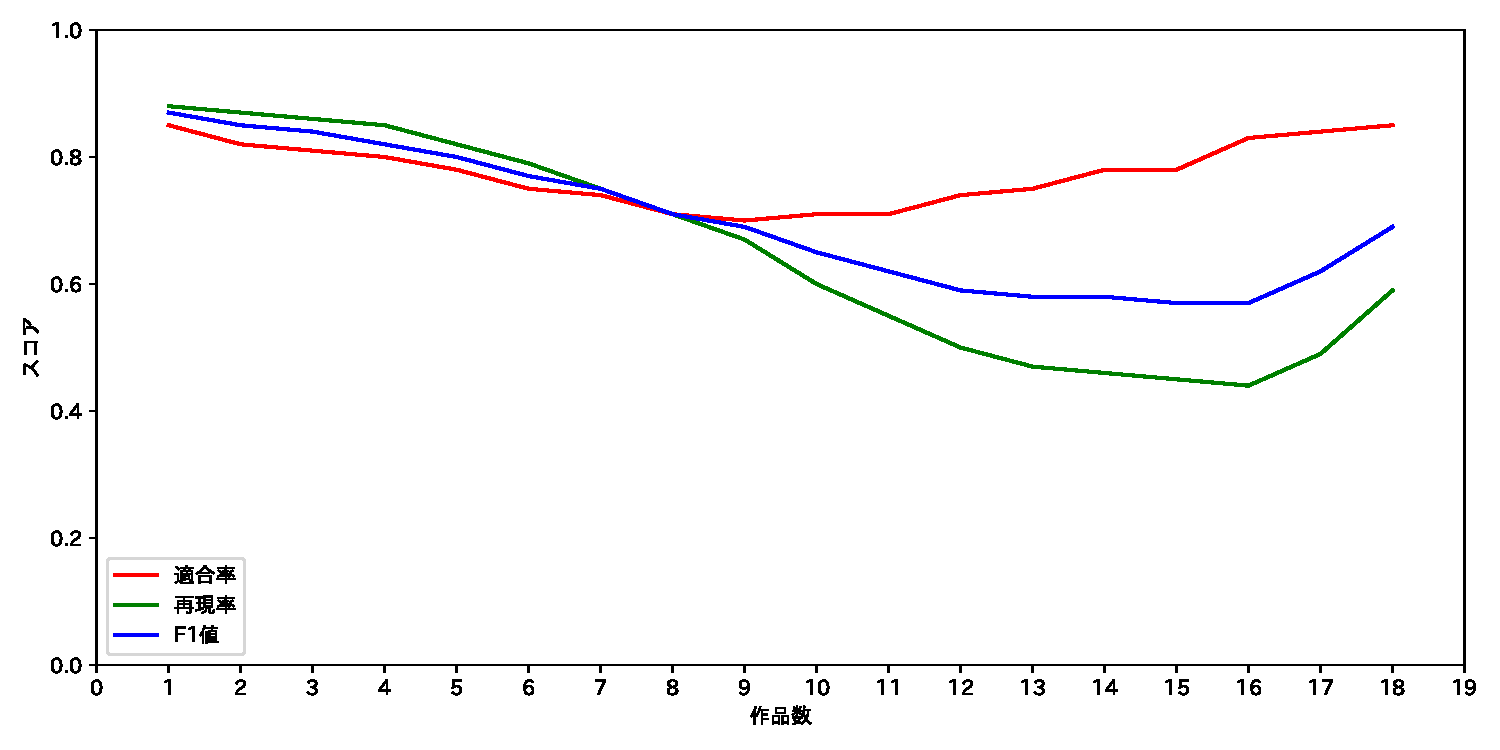
\includegraphics[width=1.0\linewidth]{Okamoto_fig/btod-lines2.pdf}
	\caption{提案BtoDモデルの作品数ごとの評価指標の遷移}
 \ecaption{Prediction performance for each number of works in BtoD model.}
	\label{fig:btod-lines}
 \vspace{-2mm}
\end{figure}

\begin{table}[t]
  \caption{従来BtoDモデルと提案BtoDモデル(L=1)の精度比較}
  \ecaption{Prediction performance between previous BtoD model and our proposed BtoD model (L=1)}
  \label{tab:btod-model-comp}
  \vspace{1mm}
  \centering
  \scalebox{0.85}{
  % \begin{tabular}{l|c|c|c|c|c}
  %   \hline
  %    & 適合率 & 再現率 & F1値 & \begin{tabular}[c]{@{}c@{}}正確に予測した\\ユーザ数\end{tabular} & \begin{tabular}[c]{@{}c@{}}誤予測した\\ユーザ数\end{tabular}\\
  %   \hline
  %   \hline
  %   従来BtoD & 0.84 & 0.86 & 0.85 & 2,333 & 370\\
  %   \hline
  %   提案BtoD & \textbf{0.85} & \textbf{0.88} & \textbf{0.87}  & 2,388 & 315\\
  %   (L=1) &  &  &  &  & \\
  %   \hline
  % \end{tabular}
  \begin{tabular}{l|c|c|c|c}
    \hline\hline
     & 適合率 & 再現率 & F値 & \begin{tabular}[c]{@{}c@{}}誤予測したユーザ数\end{tabular}\\
    \hline
    従来BtoD & 0.84 & 0.86 & 0.85 & 370\\
    \hline
    提案BtoD(L=1)& \textbf{0.85} & \textbf{0.88} & \textbf{0.87}  & 315\\
    \hline
  \end{tabular}
  }
   \vspace{-2mm}
\end{table}

\vspace{-2mm}
\subsection{予測結果}

\subsubsection{ランダムフォレストモデル}\label{sec:randResult}

% 本節では,2つの習熟度到達予測モデル(BtoDモデル,DtoMモデル)のうち,説明変数として与える遡る作品数$L$別の精度評価と,従来モデルとの精度比較,および分類精度に寄与する説明変数を述べる.


\begin{figure}[t]
	\centering
	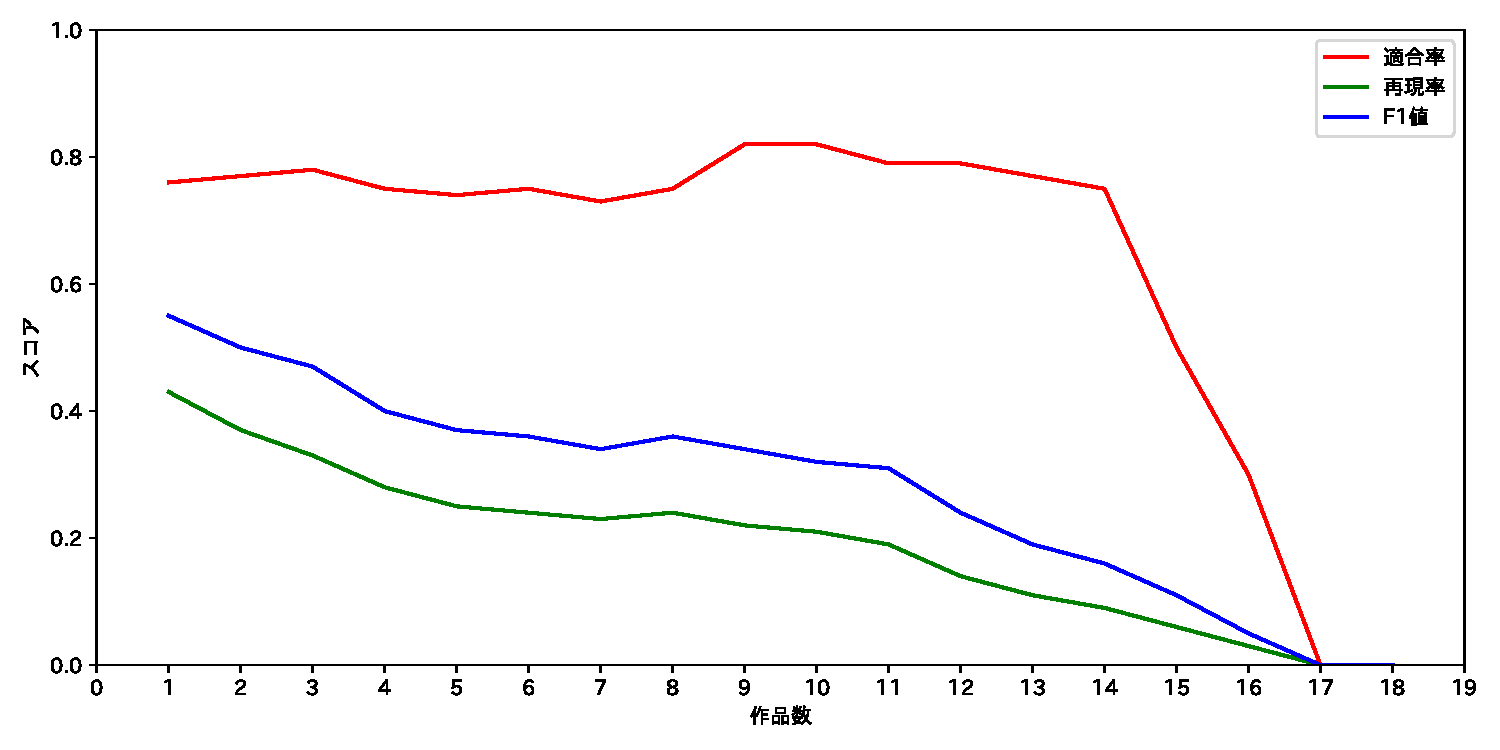
\includegraphics[width=1.0\linewidth]{Okamoto_fig/dtom-lines2.pdf}
	\caption{提案DtoMモデルの作品数ごとの評価指標の遷移}
 \ecaption{Prediction performance for each number of works in DtoM model.}
	\label{fig:dtom-lines}
  \vspace{-2mm}
\end{figure}

\begin{table}[t]
  \caption{従来DtoMモデルと提案DtoMモデル(L=1)の精度比較}
  \ecaption{Prediction performance between the previous DtoM model and our proposed DtoM model (L=1)}
  \label{tab:dtom-model-comp}
  \vspace{2mm}
  \centering
  \scalebox{0.85}{   
  \begin{tabular}{l|c|c|c|c}
    \hline\hline
     & 適合率 & 再現率 & F値 & \begin{tabular}[c]{@{}c@{}}誤予測したユーザ数\end{tabular}\\
    \hline
    従来DtoM & 0.70 & \textbf{0.44} & 0.54 & 207 \\
    \hline
    提案DtoM(L=1) & \textbf{0.79} & \textbf{0.44} & \textbf{0.57} & 144 \\
    \hline
  \end{tabular}
  }
   \vspace{-2mm}
\end{table}


\begin{table*}[t]
    \caption{従来BtoDモデルと提案BtoDモデル(L=1)における重要度の高い説明変数3件}
    \ecaption{Top 3 important explanatory variables in the previous BtoD model and our proposed BtoD model (L=1)}
    \label{tab:feature_importance-btod}
    \centering
    \scalebox{0.82}{
        \begin{tabular}{r|rp{60mm}|rp{60mm}}
            \hline\hline
            & \multicolumn{2}{c|}{従来BtoDモデル} & \multicolumn{2}{c}{提案BtoDモデル(L=1)} \\ \cline{2-5}
            グループ & \begin{tabular}{r} 重要度 \end{tabular} & \begin{tabular}{c} 説明変数 \end{tabular} & \begin{tabular}{r} 重要度 \end{tabular} & \begin{tabular}{c} 説明変数 \end{tabular} \\ \hline 
            1 & \begin{tabular}{r}0.05\end{tabular} & \begin{tabular}{r} \{オリジナル/フロー制御/0点\} \end{tabular} & \begin{tabular}{r} 0.20 \end{tabular} & \begin{tabular}{l} \{パス遷移確率P_{n-1,n} \} \end{tabular} \\ \hline
            2 & \begin{tabular}{r} 0.04 \end{tabular} & \begin{tabular}{r} \{リミックス/抽象化/0点\} \end{tabular} & \begin{tabular}{r} 0.04 \end{tabular} & \begin{tabular}{l} \{リミックス/データ表現/0点\} \end{tabular} \\ \hline
            3 & \begin{tabular}{r} 0.04 \end{tabular} & \begin{tabular}{r} \{オリジナル/データ表現/0点\} \end{tabular} & \begin{tabular}{r} 0.03 \end{tabular} & \begin{tabular}{l} \{オリジナル/ユーザ対話性/0点\} \end{tabular} \\ \hline
            % 4 & \begin{tabular}{r} 0.04 \end{tabular} & \begin{tabular}{r} \{オリジナル/ユーザ対話性/0点\} \end{tabular} & \begin{tabular}{r} 0.03 \end{tabular} & \begin{tabular}{l} \{オリジナル/フロー制御/0点\} \end{tabular} \\ \hline
            % 5 & \begin{tabular}{r} 0.04 \end{tabular} & \begin{tabular}{r} \{リミックス/並列/0点\} \end{tabular} & \begin{tabular}{r} 0.03 \end{tabular} & \begin{tabular}{l} \{リミックス/抽象化/2点\} \end{tabular} \\ \hline
            % 6 & \begin{tabular}{r} 0.04 \end{tabular} & \begin{tabular}{r} \{リミックス/データ表現/0点\} \end{tabular} & \begin{tabular}{r} 0.03 \end{tabular} & \begin{tabular}{l} \{リミックス/並列/0点\} \end{tabular} \\ \hline
            % 7 & \begin{tabular}{r} 0.04 \end{tabular} & \begin{tabular}{r} \{リミックス/抽象化/2点\} \end{tabular} & \begin{tabular}{r} 0.03 \end{tabular} & \begin{tabular}{l} \{オリジナル/データ表現/0点\} \end{tabular} \\ \hline
            % 8 & \begin{tabular}{r} 0.03 \end{tabular} & \begin{tabular}{r} \{リミックス/同期/0点\} \end{tabular} & \begin{tabular}{r} 0.03 \end{tabular} & \begin{tabular}{l} \{リミックス/抽象化/0点\} \end{tabular} \\ \hline
            % 9 & \begin{tabular}{r} 0.03 \end{tabular} & \begin{tabular}{r} \{リミックス/フロー制御/1点\} \end{tabular} & \begin{tabular}{r} 0.03 \end{tabular} & \begin{tabular}{l} \{リミックス/同期/0点\} \end{tabular} \\ \hline
            % 10 & \begin{tabular}{r} 0.03 \end{tabular} & \begin{tabular}{r} \{リミックス/論理/3点\} \end{tabular} & \begin{tabular}{r} 0.03 \end{tabular} & \begin{tabular}{l} \{リミックス/フロー制御/1点\} \end{tabular} \\ \hline
        \end{tabular}
        }
    \vspace{3mm}

    \caption{従来DtoMモデルと提案DtoMモデル(L=1)における重要度の高い説明変数3件}
    \ecaption{Top 3 important explanatory variables in the previous DtoM model and our proposed DtoM model (L=1)}
    \label{tab:feature_importance-dtom}
    \centering
    \scalebox{0.82}{
        \begin{tabular}{r|rp{60mm}|rp{60mm}}
            \hline\hline
            & \multicolumn{2}{c|}{従来DtoMモデル} & \multicolumn{2}{c}{提案DtoMモデル(L=1)} \\ \cline{2-5}
            グループ & \begin{tabular}{r} 重要度 \end{tabular} & \begin{tabular}{c} 説明変数 \end{tabular} & \begin{tabular}{r} 重要度 \end{tabular} & \begin{tabular}{c} 説明変数 \end{tabular} \\ \hline 
            1 & \begin{tabular}{r} 0.04 \end{tabular} & \begin{tabular}{l} \{オリジナル/データ表現/0点\} \end{tabular} & \begin{tabular}{r} 0.12 \end{tabular} & \begin{tabular}{l} \{パス遷移確率P_{n-1,n}\} \end{tabular} \\ \hline
            2 & \begin{tabular}{r} 0.04 \end{tabular} & \begin{tabular}{r} \{オリジナル/抽象化/0点\} \end{tabular} & \begin{tabular}{r} 0.05 \end{tabular} & \begin{tabular}{l} \{オリジナル/同期/2点\} \end{tabular} \\ \hline
            3 & \begin{tabular}{r} 0.03 \end{tabular} & \begin{tabular}{r} \{オリジナル/同期/2点\} \end{tabular} & \begin{tabular}{r} 0.04 \end{tabular} & \begin{tabular}{l} \{オリジナル/抽象化/0点\} \end{tabular} \\ 
            % 4 & \begin{tabular}{r} 0.03 \end{tabular} & \begin{tabular}{r} \{オリジナル/フロー制御/3点\} \end{tabular} & \begin{tabular}{r} 0.03 \end{tabular} & \begin{tabular}{l} \{オリジナル/データ表現/0点\} \end{tabular} \\ \hline
            % 5 & \begin{tabular}{r} 0.03 \end{tabular} & \begin{tabular}{r} \{リミックス/同期/0点\} \end{tabular} & \begin{tabular}{r} 0.03 \end{tabular} & \begin{tabular}{l} \{リミックス/同期/0点\} \end{tabular} \\ 
            \hline
            % 6 & \begin{tabular}{r} 0.03 \end{tabular} & \begin{tabular}{l} \{オリジナル/論理/0点\} \\ \{オリジナル/フロー制御/1点\} \\ \{リミックス/論理/0点\} \end{tabular} & \begin{tabular}{r} 0.03 \end{tabular} & \begin{tabular}{l} \{オリジナル/フロー制御/3点\} \end{tabular} \\ \hline
            % 7 & \begin{tabular}{r} 0.03 \end{tabular} & \begin{tabular}{r} \{オリジナル/並列/3点\} \end{tabular} & \begin{tabular}{r} 0.03 \end{tabular} & \begin{tabular}{l} \{オリジナル/並列/3点\} \end{tabular} \\ \hline
            % 8 & \begin{tabular}{r} 0.03 \end{tabular} & \begin{tabular}{r} \{オリジナル/同期/3点\} \end{tabular} & \begin{tabular}{r} 0.03 \end{tabular} & \begin{tabular}{l} \{オリジナル/データ表現/2点\} \end{tabular} \\ \hline
            % 9 & \begin{tabular}{r} 0.03 \end{tabular} & \begin{tabular}{r} \{リミックス/フロー制御/1点\} \end{tabular} & \begin{tabular}{r} 0.03 \end{tabular} & \begin{tabular}{l} \{オリジナル/並列/2点\} \\ \{リミックス/並列/0点\} \end{tabular} \\ \hline
            % 10 & \begin{tabular}{r} 0.03 \end{tabular} & \begin{tabular}{r} \{オリジナル/論理/2点\} \end{tabular} & \begin{tabular}{r} 0.03 \end{tabular} & \begin{tabular}{l} \{オリジナル/同期/3点\} \end{tabular} \\ 
            % \hline
        \end{tabular}
    }
    \vspace{-4mm}
\end{table*}

図\ref{fig:btod-lines}は,BtoDモデルにおいて予測時から遡る作品数$L$別の予測結果(適合率,再現率,F値)を示す.横軸は作品数$L$,縦軸は各予測評価値を示す.各分類精度は,層化10分割交差検証により出力した10回分の精度の平均値を表している.BtoDモデルの評価指標はノード数$L=1$のときに最も高いF1値となり,適合率は0.85,再現率は0.88,F1値は0.87であった.表\ref{tab:btod-model-comp}は従来BtoDモデルと提案BtoDモデル($L=1$)の予測結果,非BtoDユーザと誤って予測したBtoDユーザ数を示す.従来手法に比べてわずかに高い精度で予測することができた.具体的には,従来手法でDeveloping以上に到達したユーザ55人(=370人-315人)の誤分類が提案BtoDモデルによって減少した.\textcolor{red}{\UnderlineTex{[変更2-10-a]したがって,Deveolopingに到達するユーザがDeveolopingの直前に制作する作品で共通のCT概念を使用する作品を制作していることが示唆される.また,同様にDeveolopingに到達しないユーザも20作品目の直前に制作する作品で共通のCT概念を使用する作品を制作していることが示唆される.}}


%図\ref{fig:btod-lines}は,構築したBtoDモデルにおいて作品間ノード数$L$ごとの分類精度(適合率,再現率,F値)を示す.横軸は予測する作品から遡るノード数$L$,縦軸は予測精度(適合率,再現率,F1値),を示す.
%各分類精度は,層化10分割交差検証により出力した10回分の精度の平均値を表している.BtoDモデルの評価指標はノード数$L=1$のときに最も高い数値となり,適合率は0.85,再現率は0.88,F値は0.87であった.表\ref{tab:btod-model-comp}は従来BtoDモデルと提案BtoDモデルのうち,最も精度の高かったノード数$L=1$の分類精度と正しく予測されたBtoDユーザ数,誤って非BtoDユーザであると予測されたBtoDユーザ数を示す.
% 従来BtoDモデルではDeveloping以上に到達したユーザに対して正しく予測できた数が2,333であるのに対し,提案BtoDモデルでは2,388であることから,提案BtoDモデルによって55人の習熟度向上ユーザが正しく予測できるようになったといえる.また,従来BtoDモデルではDeveloping以上に到達したユーザに対して到達していないと誤分類されたユーザ数が370であるのに対し,提案BtoDモデルでは315であることから,提案BtoDモデルによって55人のDeveloping以上に到達したユーザに対して誤分類が減ったといえる.従来BtoDモデルの適合率は0.84,再現率は0.86,F1値は0.85であり,提案BtoDモデルの適合率は0.85,再現率は0.88,F1値は0.87であることから,提案BtoDモデルは従来BtoDモデルと比べて適合率,再現率,F値において上回っているため,Developingに到達するユーザは直近に同じCT概念を持つ作品を制作することが多く,一度もDevelopingに到達しなかったユーザは直近に異なるCT概念を持つ作品を制作することが多いことが示唆される.

図\ref{fig:dtom-lines}は,BtoDモデルと同じ形式でDtoMモデルの結果を示す.DtoMモデルの評価指標はノード数$L=1$のときに最も高いF1値となり,適合率は0.79,再現率は0.44,F1値は0.57であった.
\color{red}
\UnderlineTex{[変更1-2-4][変更C2-3]表9
%\ref{tab:dtom-model-comp}
は従来DtoMモデルと提案DtoMモデル($L=1$)の予測結果を示す.}
\color{black}
従来手法に比べて高い精度で予測することができた.具体的には,従来手法で\textcolor{red}{\UnderlineTex{Developing}}以上に到達したユーザ63人(=207人-144人)の誤分類が提案DtoMモデルによって減少した.\textcolor{red}{\UnderlineTex{[変更2-10-b]したがって,Masterに到達するユーザがMasterの直前に制作する作品で共通のCT概念を使用する作品を制作していることが示唆される.また,同様にMasterに到達しないユーザも20作品目の直前に制作する作品で共通のCT概念を使用する作品を制作していることが示唆される.}}


% 図\ref{fig:dtom-lines}は,構築したDtoMモデルにおいて作品間ノード数$L$ごとの分類精度(適合率,再現率,F値)を示す.縦軸は評価スコア,横軸は作品間ノード数$L$を意味する.各分類精度は,層化10分割交差検証により出力した10回分の精度の平均値を表している.BtoDモデルの適合率はノード数$L=9$のときに最も高い0.80となり,再現率,F値はノード数$L=1$のときに最も高くなり,それぞれ0.43,0.55であった.表\ref{tab:dtom-model-comp}は従来DtoMモデルと提案DtoMモデルのうち,最もF値が高かったノード数$L=1$の分類精度と習熟度が向上したと予測された非BtoDユーザ数を示す.従来DtoMモデルではMaster以上に到達したユーザに対して到達していないと誤分類されたユーザ数が207であるのに対し,提案DtoMモデルでは144であることから,提案DtoMモデルによって63人のMasterに到達しなかったユーザに対して誤分類が減ったといえる.従来DtoMモデルの適合率は0.70,再現率は0.44,F1値は0.54であり,提案DtoMモデルの適合率は0.77,再現率は0.45,F1値は0.59であった.従来DtoMモデルと比べて提案DtoMモデルは適合率,F値において上回っているため,BtoDモデルと同様に,Masterに到達するユーザは直近に同じCT概念を持つ作品を制作することが多く,一度もMasterに到達しなかったユーザは直近に異なるCT概念を持つ作品を制作することが多いことが示唆される.



表\ref{tab:feature_importance-btod}と表\ref{tab:feature_importance-dtom}はそれぞれ従来BtoDモデルと提案BtoDモデル,従来DtoMモデルと提案DtoMモデルにおいて,予測精度に寄与した説明変数の結果を示す.重要度の値は,層化10分割交差検証により出力した10回分の重要度の平均値を示す.また,予測精度に寄与する説明変数はCT概念の場合,\{作品の種類/CT概念,点数\}のように示す.BtoDモデル,DtoMモデルは,いずれも本研究で提案する説明変数\{遷移確率$P_{m-1,m}$\}が予測精度に最も寄与しており,特定の習熟度に到達する直前の作品で使用するCTスコアが予測に有用であることが明らかとなった.



% 表\ref{tab:feature_importance-btod}より,従来BtoDモデルでは,説明変数\{オリジナル/フロー制御/0点\}が分類精度に最も寄与し,続いて\{リミックス/抽象化/0点\},\{オリジナル/データ表現/0点\}が寄与しているのに対し,提案BtoDモデルでは本実験で提案した説明変数\{遷移確率$P_{m-1,m}$\}が分類精度に最も寄与し,続いて\{リミックス/データ表現/0点\},\{オリジナル/ユーザ対話性/0点\}が寄与していることがわかった.

% 表\ref{tab:feature_importance-dtom}より,従来DtoMモデルでは,説明変数\{オリジナル/データ表現/0点\}が分類精度に最も寄与し,続いて\{オリジナル/抽象化/0点\},\{オリジナル/同期/2点\}が寄与しているのに対し,提案BtoDモデルでは本実験で提案した説明変数\{遷移確率$P_{m-1,m}$\}が分類精度に最も寄与し,続いて\{オリジナル/同期/2点\},\{オリジナル/抽象化/0点\}が寄与していることがわかった.

% 従来BtoDモデルと従来DtoMモデルにおいて最も分類精度に寄与した説明変数と次に重要度の大きい説明変数との重要度の差はどちらも0.01程度であったが,提案BtoDモデルにおいて最も分類精度に寄与した\{遷移確率$P_{m-1,m}$\}の重要度は次に大きい\{リミックス/データ表現/0点\}の重要度の約5倍,また提案BtoDモデルにおいて最も分類精度に寄与した\{遷移確率$P_{m-1,m}$\}の重要度は次に大きい\{オリジナル/同期/2点\}の重要度の約2.4倍であることから,本提案モデルで用いた説明変数は予測に対して有効に働き,重要な指標であることが示唆される.



\subsubsection{N階マルコフ連鎖モデル}\label{sec:markovResult}

図\ref{fig:markov-btod}は,それぞれ階数N毎のBtoDモデルとDtoMモデルの分類精度(適合率,再現率,F1値)を折れ線グラフで,\ref{sec:marcov-approach}項で述べたとおり予測対象となるユーザが過去に制作した作品のCTパスが学習データに含まれていないため予測できなかったユーザ数(灰色),予測できたが不正解だったユーザ数(青色),予測できて正解したユーザ数(橙色)をそれぞれ積み上げ棒グラフで示す.折れ線グラフの縦軸(左)は予測評価値,積み上げ棒グラフの縦軸(右)はユーザ数,横軸はN階マルコフ連鎖モデルの階数Nを表す.各評価指標は,層化10分割交差検証により出力した10回分の精度の平均値を表し,ユーザ数は層化10分割交差検証により出力した10回分のユーザ数の合計を表している.

図\ref{fig:markov-btod}より,BtoDモデルの評価指標は階数が大きくなるにつれてF1値は向上した.また,DtoMモデルでは階数の大きさに伴いわずかにF1値が向上する程度で,階数が$N=8$のときにF1値が最高値($0.65$)であった.本手法は,従来手法では特定の習熟度に到達するまでのCTパスを考慮していなかったことが原因で誤って予測していたユーザの習熟度到達予測を改善する一方で,階数が大きくなるほど予測できるユーザ数が減少することは今後の課題である.

% \todo{予測精度が高いかどうか.ランダムフォレストに比べると低いけど,どう書くか.}\todo{予測できなかったユーザが多数いたのは,CTスキルの完全一致を考えたからで,今後は部分一致を考えて予測できるユーザを増やす方法を考える.}

%---------------------
\begin{figure*}[t]
	\centering
	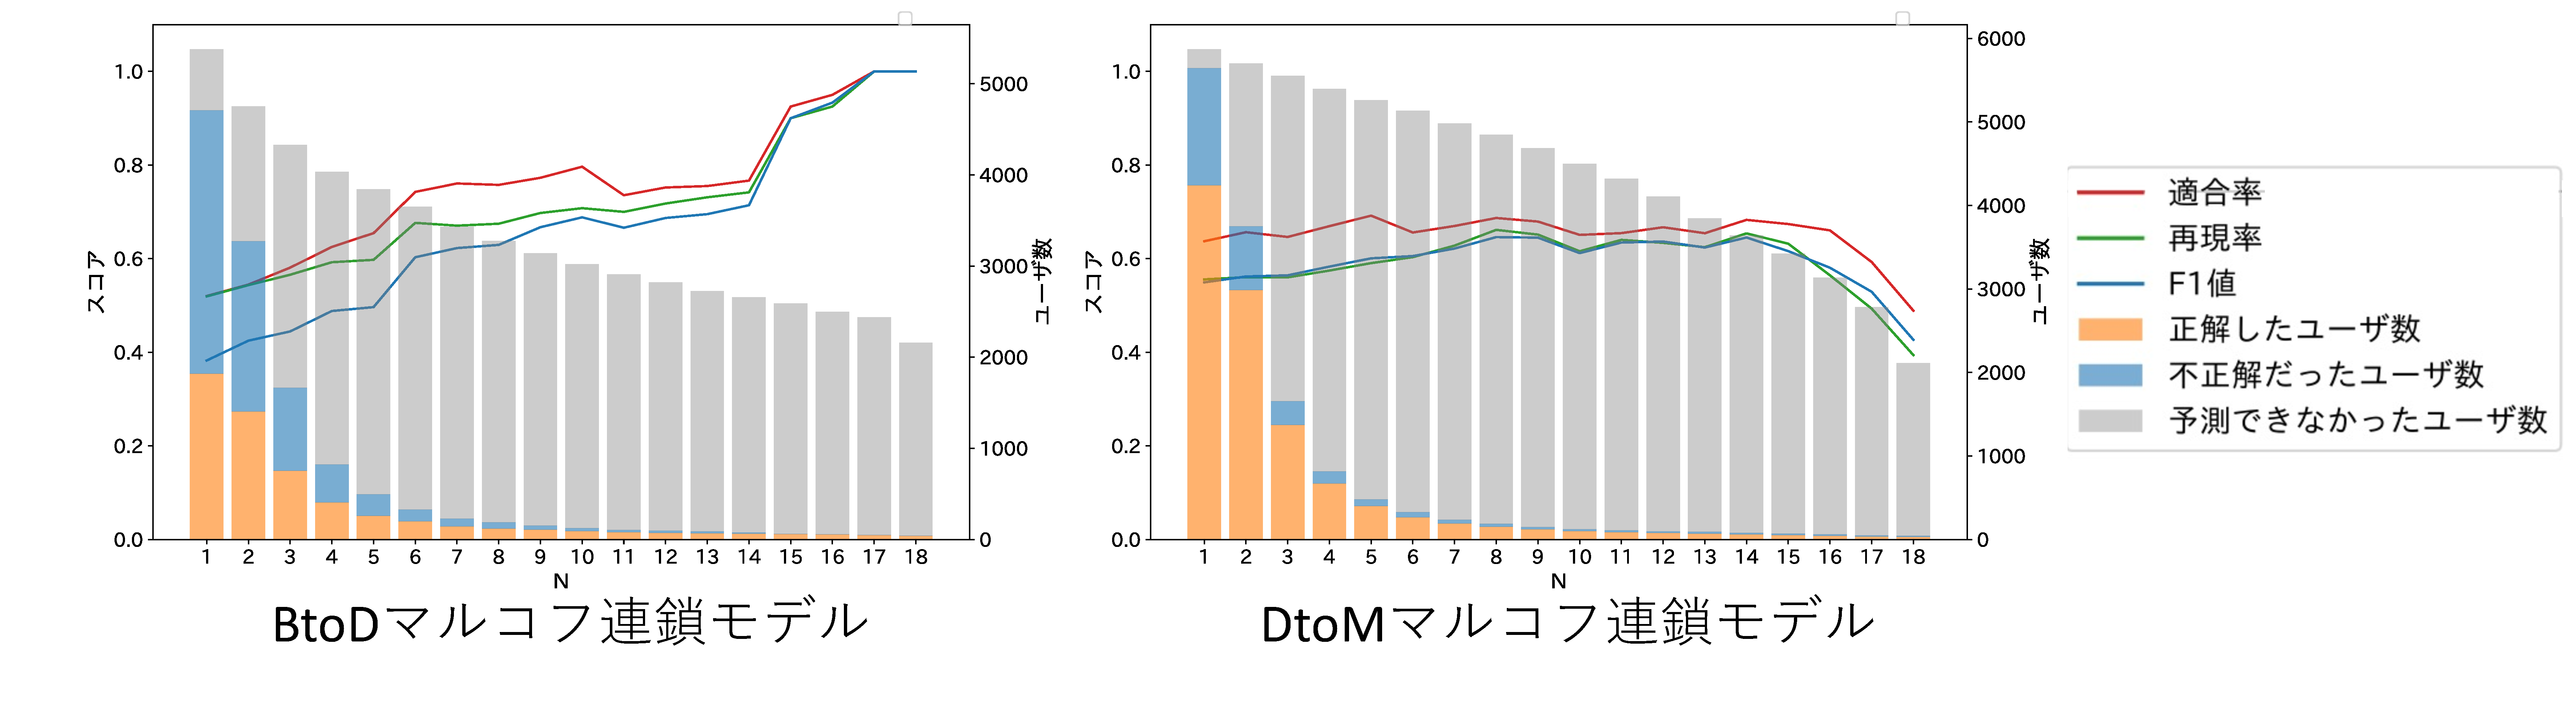
\includegraphics[width=0.9\linewidth]{Okamoto_fig/markov-result.pdf}
        \vspace{-5mm}
	\caption{階数N毎のマルコフ連鎖モデルの精度とユーザ数の分布}
 \ecaption{Prediction performance of Markov chain model for each rank (line graph) and distribution of the predicted users (bar graph)}
	\label{fig:markov-btod}
 \vspace{-4mm}
\end{figure*}
%---------------------


\vspace{-5mm}
\subsection{考察}

% 本節では,構築した習熟度到達予測を行う2つの提案モデルの評価結果に基づき,提案モデルの精度に起因する要因と,提案モデルと従来モデルで予測できた作品の特徴について考察する.

\subsubsection{予測精度に起因する要因}

\ref{sec:randResult}項で示した通り,2種類のランダムフォレストモデルでは予測する作品から遡る作品数が1つ($L=1$)の時に予測評価値が最も高く,また\ref{sec:markovResult}項では階数が小さいほどより多くのユーザに対して予測することが可能であることを確認した.したがって,特定の習熟度に到達するユーザと到達しないユーザ間では,作品$n-1$から作品$n$へのCTパス重複数に違いがあることが示唆される.図\ref{fig:add-btod}はそれぞれ特定の習熟度に到達したユーザ(BtoDユーザ,またはDtoMユーザ)と到達しなかったユーザ(非BtoDユーザ,または非DtoMユーザ)におけるCT\textcolor{red}{\UnderlineTex{[変更1-3-22]パス}}重複数の分布を示す.BtoDユーザは非BtoDユーザよりもCTパス重複数が多く,それぞれの中央値は7.0と3.0であり,Mann–Whitney U検定(p値$<$0.05)によって統計的有意差があることを確認した.一方で,DtoMユーザは非DtoMユーザに比べてCTパス重複数が低く,\textcolor{red}{\UnderlineTex{[変更1-3-23]中央値はそれぞれ}}2.0と4.0であり統計的有意差があることを確認した.

BtoDユーザはRQ1で習熟度\textcolor{red}{\UnderlineTex{[変更1-3-5]Developing以上に到達}}するまでに制作した作品で使用するCT概念に共通性が存在することを明らかにしていることもあり,習熟度\textcolor{red}{\UnderlineTex{[変更1-3-5]Developing以上に到達}}する直前の遷移確率を使用することで予測精度が向上したことが示唆される.一方で,RQ1でDtoMユーザはBtoDユーザに比べて多様なCTパスを経由して習熟度Masterに到達しているため,習熟度\textcolor{red}{\UnderlineTex{[変更1-3-5]Developing以上に到達}}する直前の遷移確率は低いが,到達できない作品の遷移確率が高いため,非DtoMユーザを正しく分類できた結果精度が向上したことが示唆される.



% \ref{subsec:model-result}節に示された通り,2種類のランダムフォレストモデルに学習させる遷移確率$P$が1つの時に最高の精度を達成し,\ref{subsec:importance}節では,遷移確率$P$の特徴量重要度が高くなっている.また,DtoMマルコフ連鎖モデルでは階数Nが小さいときに精度が高くなっている.これらのことから,特定の習熟度に到達するユーザと到達しないユーザ間では,作品n−1から作品nへの遷移確率に差があることが示唆された.

% 図\ref{fig:add-btod}はDevelopingの習熟度に到達したユーザ(BtoDユーザ)とDevelopingに到達しなかったユーザ(非BtoDユーザ)が直前の作品に遷移する際のパスの重複数の分布を比較している.BtoDユーザの中央値は7.0,非BtoDユーザの中央値は3.0であり,Mann–Whitney U検定によって統計的に有意な差(p$<$0.05)が確認できた.これは,Developingの習熟度に到達するユーザが頻繁に通るパスを辿るのに対し,到達しないユーザはあまり再現性のないパスを通っていることが示唆された.

% また,図\ref{fig:add-dtom}はMasterの習熟度に到達したユーザ(DtoMユーザ)と,Developingに到達しなかったユーザ(非BtoDユーザ)が直前の作品に遷移する際のパスの重複数の分布を示す.DtoMユーザの中央値は2.0,非DtoMユーザの中央値は4.0であり,Mann–Whitney U検定を実施したところ,統計的に有意な差(p$<$0.05)を確認できた.Masterの習熟度に到達するユーザがより多様な作品から遷移する傾向にあること,また到達しないユーザはより再現性のあるパスを辿る傾向にあることを示している.このことから,DtoMマルコフ連鎖モデルの階数Nが小さい時に精度が高かった要因として,負クラスユーザが多かったことが挙げられる.

%---------------
\begin{figure}[t]
	\centering
	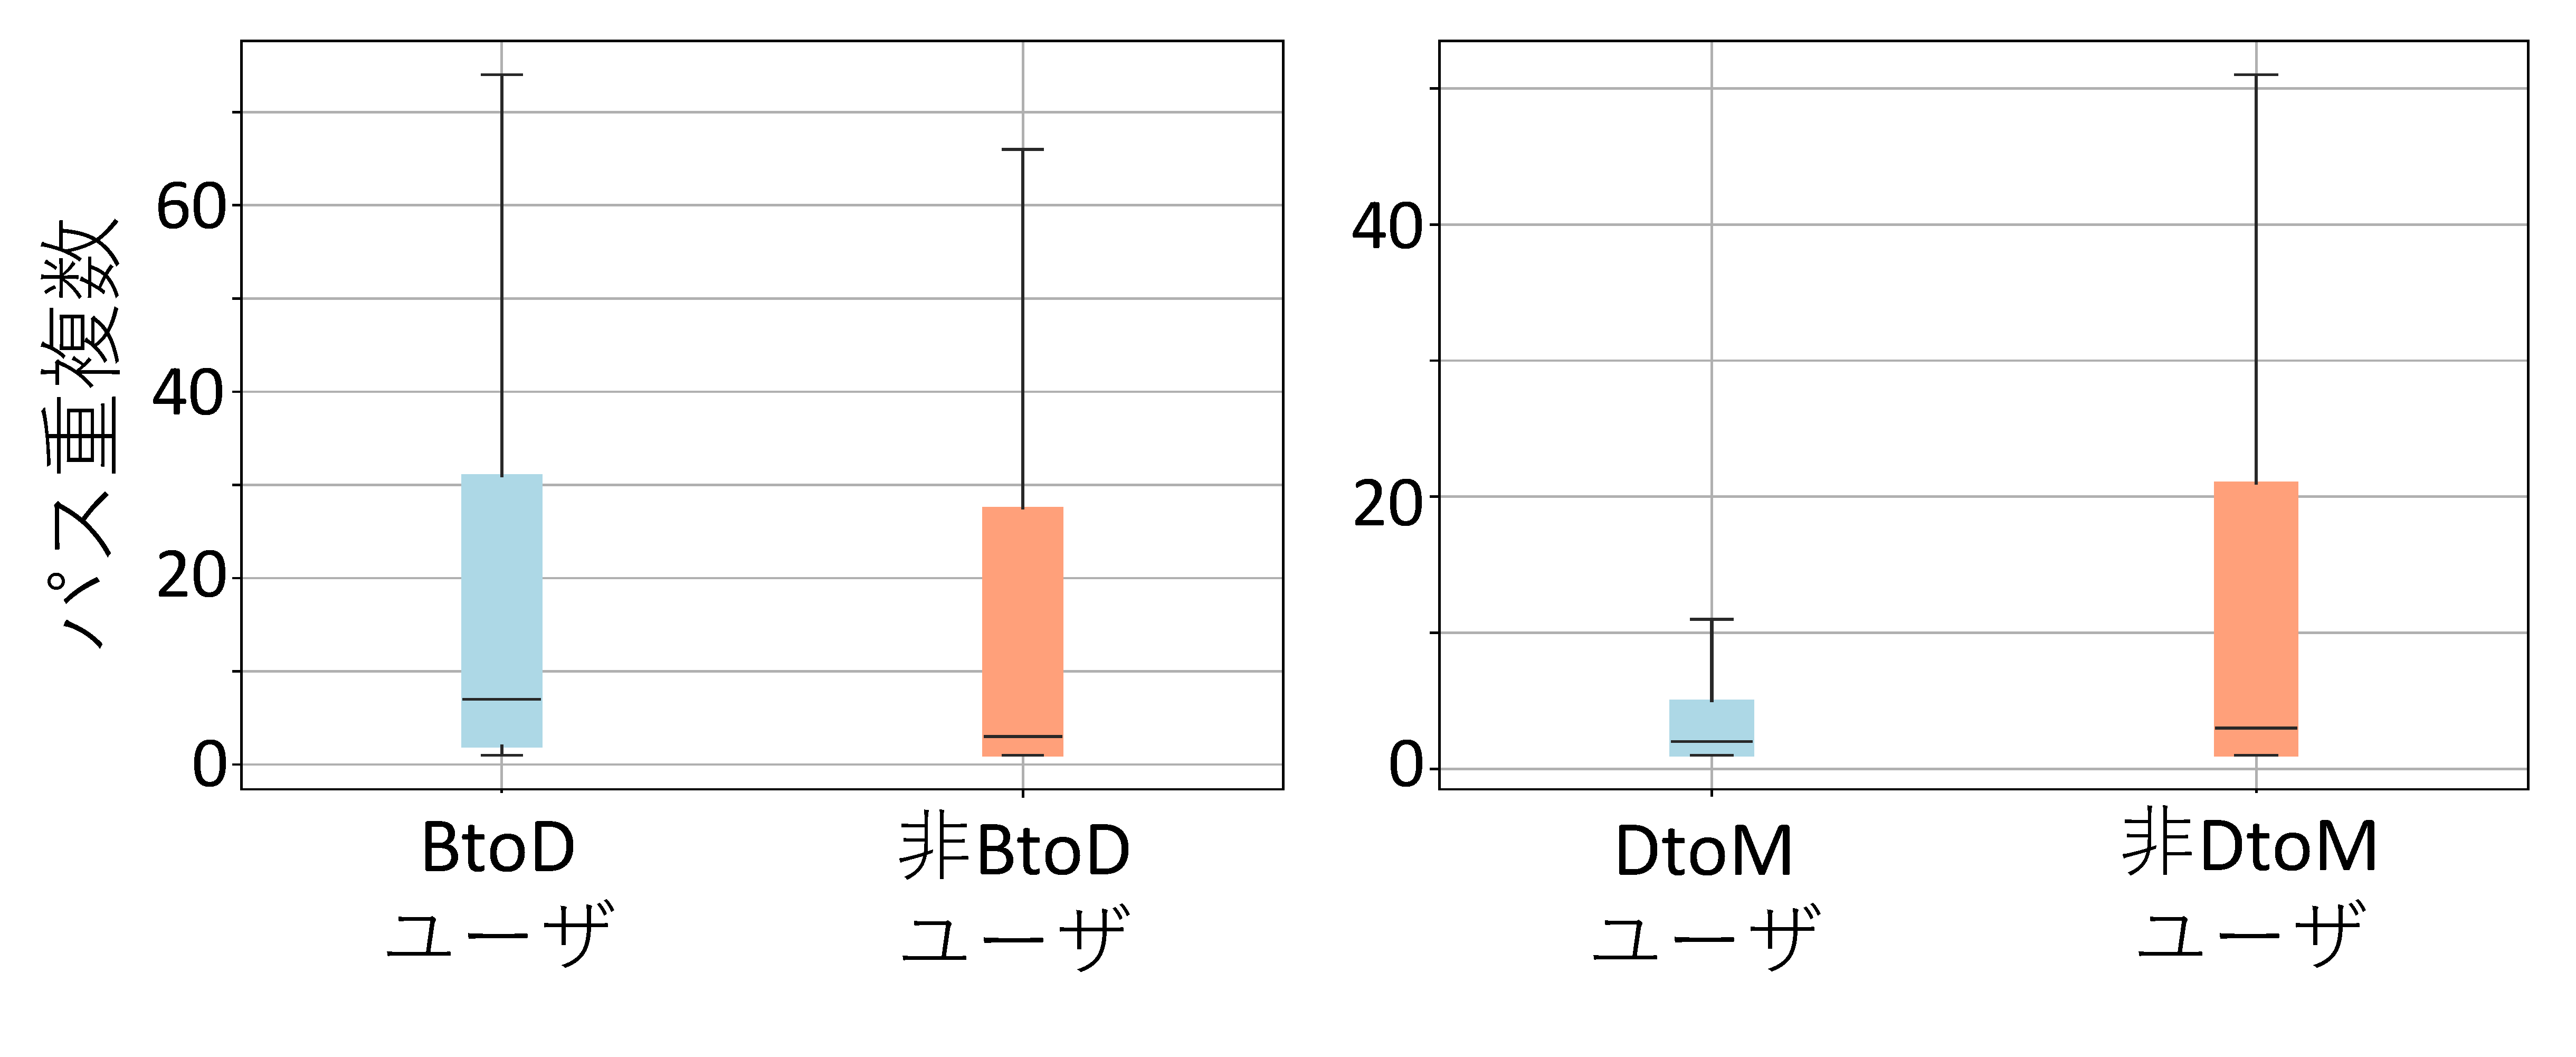
\includegraphics[width=1\linewidth]{Okamoto_fig/add-btod-dtom.pdf}
        \vspace{-7mm}
	\caption{BtoD/DtoMユーザと非BtoD/非DtoMユーザにおけるBasic/Developingの作品(N-1番目)からDeveloping/Masterの作品(N番目)のCTパス重複数}
        \ecaption{CT paths overlapping from work with Basic/Developing (N-1) to the work with Developing/Master (N) for BtoD/DtoM and non-BtoD/non-DtoM users}
	\label{fig:add-btod}

 \centering
	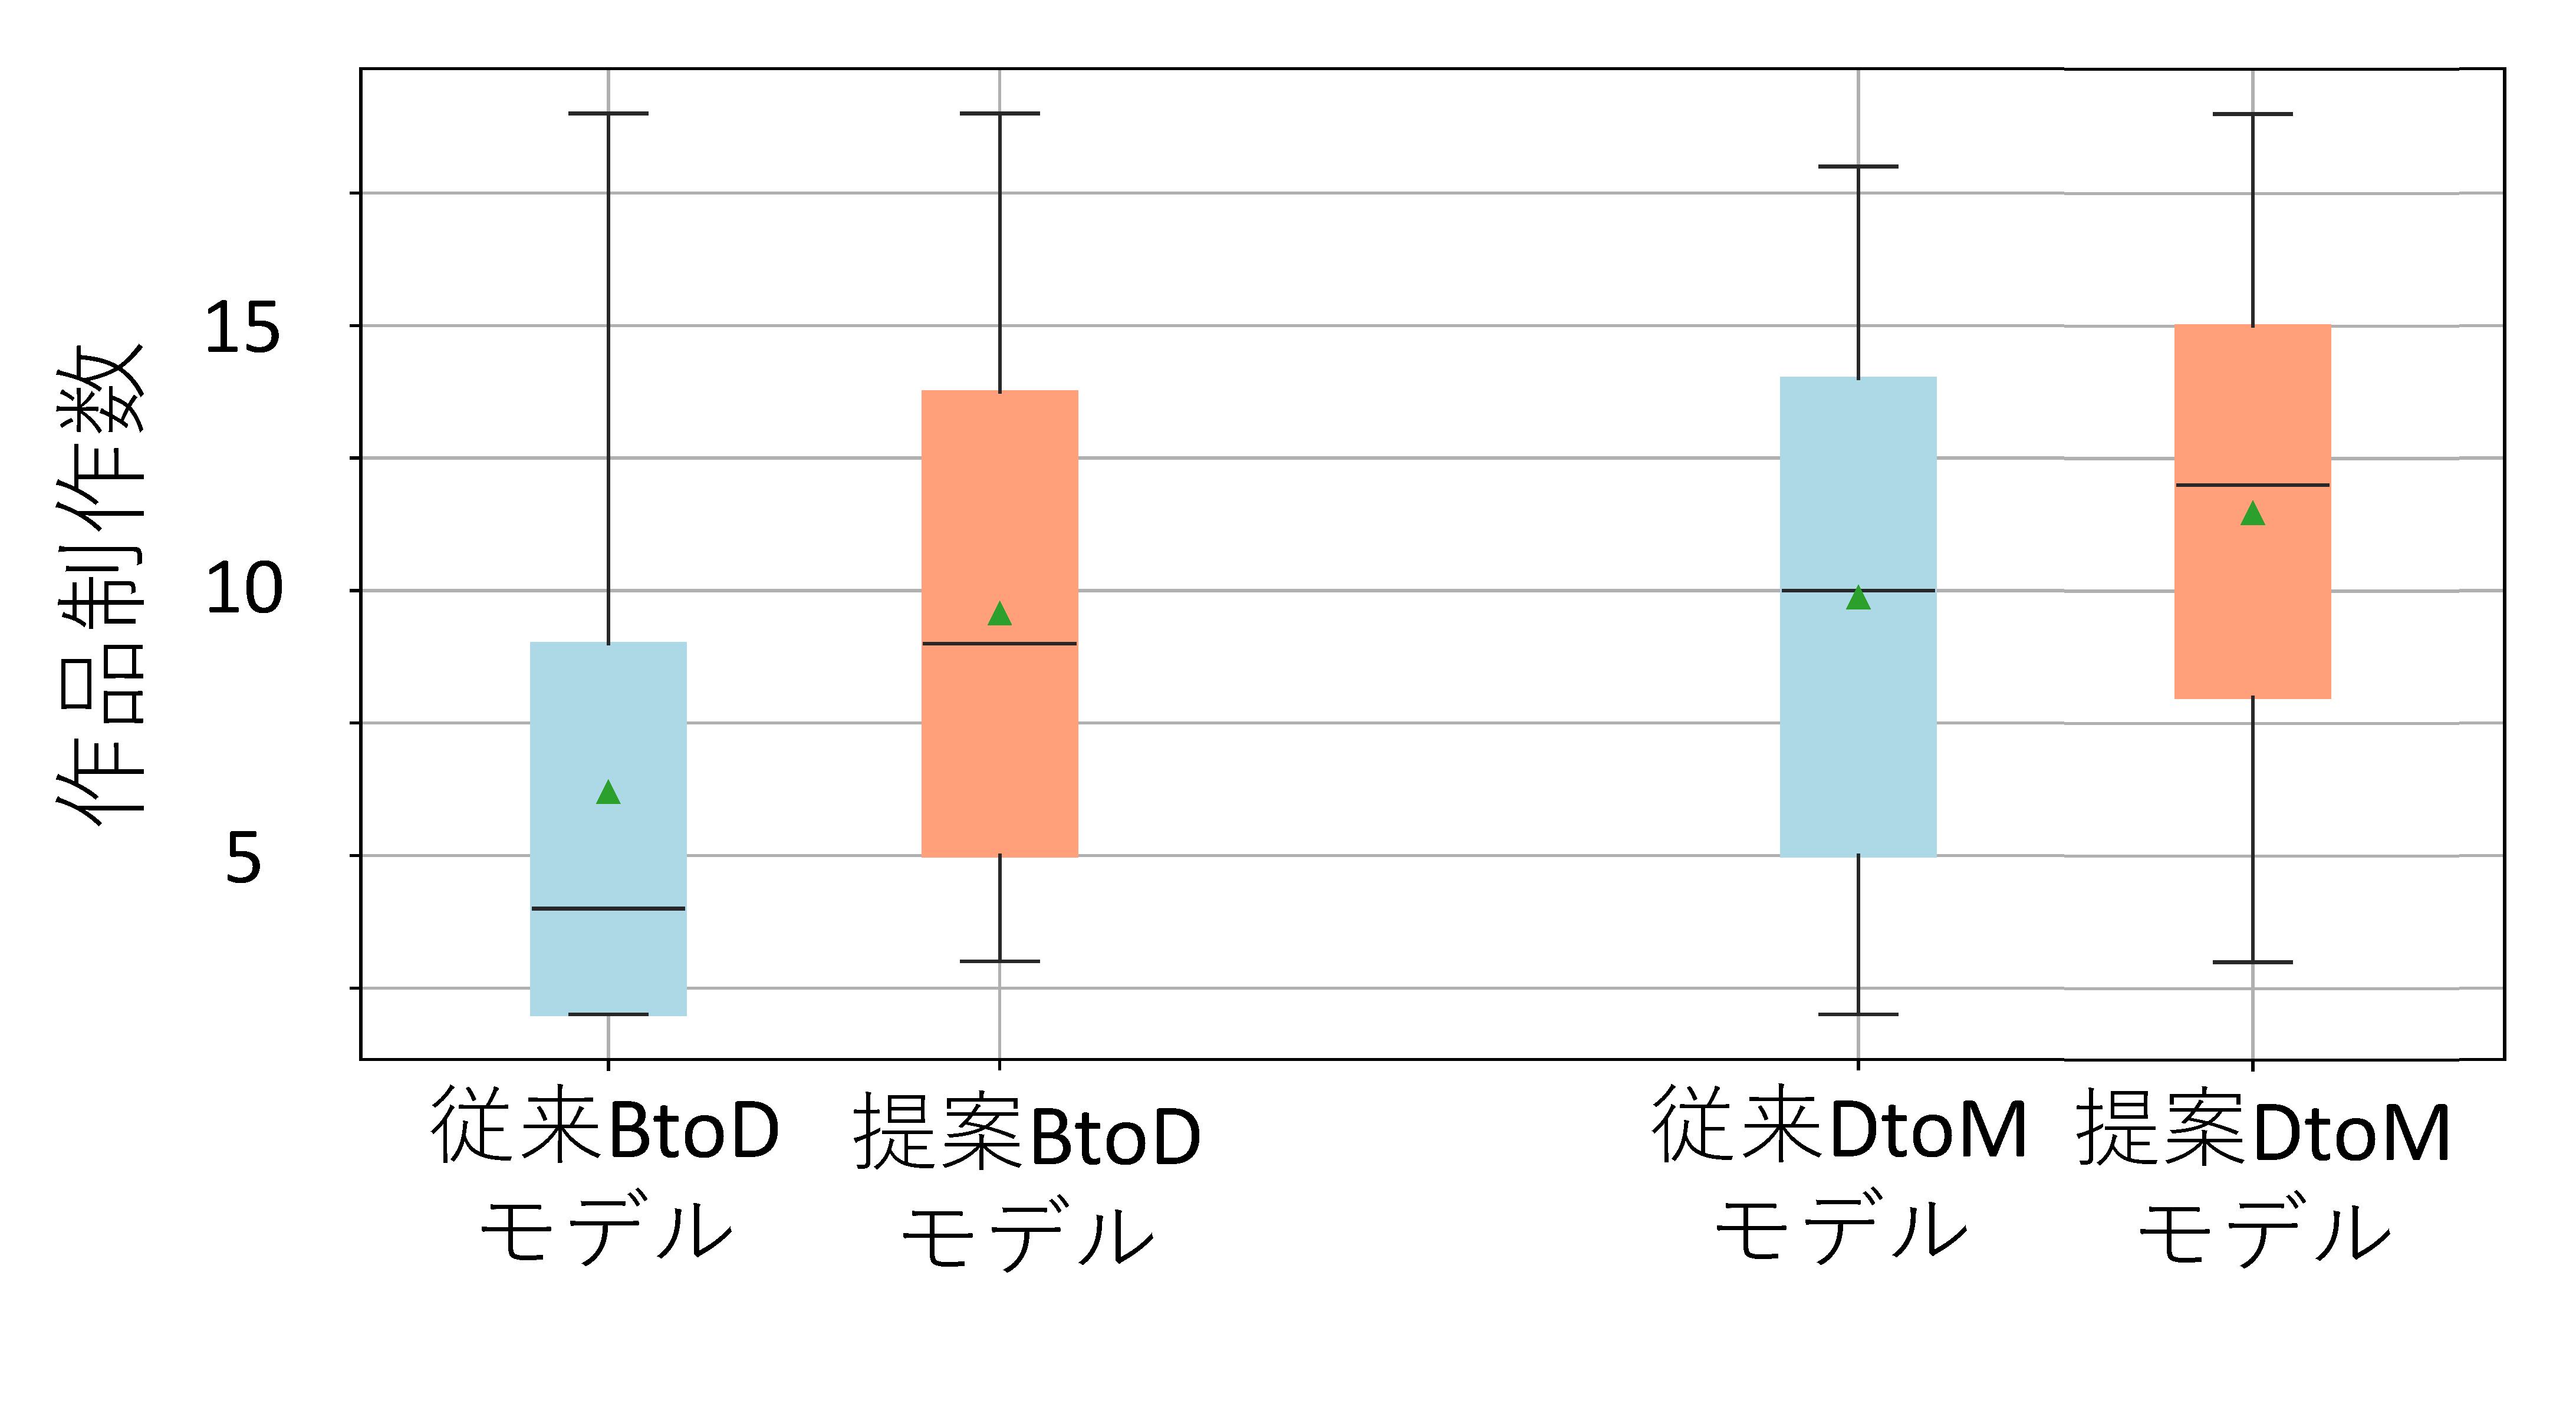
\includegraphics[width=0.75\linewidth]{Okamoto_fig/btod-dtom-path.pdf}
        %\vspace{-2mm}
	\caption{従来モデルで予測できたユーザと提案マルコフ連鎖モデルで予測できたユーザの作品制作数の分布}
        \ecaption{Distribution of the successfully predicted works between the previous model and our proposed Markov chain model.}
	\label{fig:btod-path}
    \vspace{-4mm}
\end{figure}
%---------------

% \subsection{従来モデルと提案モデルで予測できたユーザと予測できなかったユーザの特徴分析}
\subsubsection{提案モデルによる貢献可能なユーザ}

本研究が提案したモデルは,従来手法に比べて高い精度で予測できる手法であった.その理由を明らかにするために,本研究の提案手法と従来手法において,正確に予測したユーザの特徴の違いを調査する.図\ref{fig:btod-path}は従来モデルで正確に予測できた正クラスのユーザ(BtoDユーザまたはDtoMユーザ)とN階マルコフ連鎖モデルのみで正確に予測できた正クラスのユーザが制作した作品数の分布を示す.BtoDモデル,DtoMモデルともにN階マルコフ連鎖モデルが従来モデルよりも作品制作数の多いユーザの予測に成功しており,いずれもMann–Whitney U検定(p値$<$0.05)によって統計的有意差があることを確認した.したがって,本研究が提案するN階マルコフ連鎖モデルは作品制作数の多いユーザの予測に有用である一方で,作品制作数の少ないユーザは従来手法を利用する方が良いことが示唆される.

表\ref{tab:path-btod}は,従来モデルでCT概念の獲得有無のみを学習していたため誤分類されたが,N階マルコフ連鎖モデルで正しく予測されたユーザ1人を抽出し,作品のCTスコアを制作順に示す.当該ユーザはリミックス作品を制作した直後に類似のCT概念を使用したオリジナル作品を制作している.具体的には1作品目と2作品目,3作品目と4作品目,7作品目と8作品目が該当する.他のユーザでも同じような傾向が見られた.このような作品制作順序に特徴を持つ場合は,N階マルコフ連鎖モデルが有用であることが示唆される.


% \subsubsection*{ランダムフォレストモデル}

% 図\ref{fig:btod-venn}に,従来BtoDモデルと提案BtoDモデルがそれぞれ予測できたユーザの数,両モデルが共に予測できたユーザの数,および予測できなかったユーザの数を示す.提案BtoDモデルでは,CTパスが同一で予測結果も一致したユーザのペアが12組見つかったが,従来BtoDモデルのみで予測できたユーザ内にはペアは見つからなかったことから,提案BtoDモデルによってCTスキル習熟過程を考慮した習熟度の到達予測が可能にしたことが示唆された.また,従来BtoDモデルと提案BtoDモデルで予測できたユーザは作品制作数の中央値が9.0であるのに対し,どちらのモデルでも予測できなかったユーザの作品制作数の中央値は19.0であった.Mann–Whitney U検定を実施したところ,統計的な有意差(p値$<$0.05)が確認できたことから,従来BtoDモデルと提案BtoDモデルでは作品制作数の多いユーザのCTは十分に考慮できておらず,分類が困難であることが示された.

% 図\ref{fig:dtom-venn}に,従来DtoMモデルと提案DtoMモデルがそれぞれ予測できたユーザの数,両モデルが共に予測できたユーザの数,および予測できなかったユーザの数を示す.提案DtoMモデルで予測できたユーザの中でCTパスが同一で,予測結果が一致したユーザのペアは見つからなかった.このことから,\ref{sec:3-analysis}節で明らかにされた通り,DtoMユーザが多様なCTパスを通る傾向にあることを踏まえると,提案DtoMモデルではCT週を十分に考慮できていないことが示唆された.また,従来DtoMモデルと提案DtoMモデルで予測できたユーザは制作した作品数の中央値が17.0であるのに対し,どちらのモデルでも予測できなかったユーザが制作した作品数の中央値は11.0であった.Man-whitney U検定を実施したところ,統計的な有意差(p値$<$0.05)が確認できた.\ref{sec:3-analysis}節での分析により,DtoMユーザのうち,作品制作数が比較的少ないDtoMユーザの方がより多様性のあるCTパスを通る傾向にあることが明らかとなったことから,従来DtoMモデルと提案DtoMモデルでは作品制作数の比較的少ないユーザのCT習熟過程は十分に考慮できていないことが示された.


% 図\ref{fig:btod-path}は,従来BtoDモデルのみで予測できた正クラスのユーザ(BtoDユーザ)とBtoDマルコフ連鎖モデルのみで予測できた正クラスのユーザが制作した作品数の分布を示す.従来モデルのBtoDユーザの中央値は4.0,マルコフ連鎖モデルのBtoDユーザの中央値は9.0であり,Man-whitney U検定を実施したところ,統計的に有意な差(p$<$0.05)を確認できた.このことから,提案マルコフ連鎖モデルでは,従来モデルよりもより作品制作数の多いユーザの予測が可能になったことを示しており,逆に作品制作数の少ないユーザの予測は従来モデルが適していることがわかる.

% 表\ref{tab:path-btod}はBtoDモデルの予測結果が正解したBtoDユーザの中から,従来モデル\todo{従来ランダム?提案ランダム?}では\todo{XXが理由で}予測結果が外れていたユーザを1人抽出し,作品のCTスコアを制作順に示す.
% 当該ユーザは7作品目で習熟度Developingに到達している.表\ref{tab:path-btod}で抽出されたユーザはリミックス作品を制作した直後にほとんど同じCT概念を持つ作品を制作する傾向にある.



例えば,3作品目のリミックス作品を制作した直後の4作品目では全く同じCT概念を持つ作品を制作している.点数は若干異なるが,1,2作品目,7,8作品目でも同じような傾向が見られる.また,他にも数件このようなケースが見られたため,本モデルはRQ1のBtoDユーザのCTスキル習熟過程の分析結果で得られたような,繰り返し同じCT概念の作品を制作するユーザの特徴を捉え,予測が可能になっていることが示唆された.

% 図\ref{fig:btod-path}は,従来DtoMモデルのみで予測できた正クラスのユーザ(DtoMユーザ)とDtoMマルコフ連鎖モデルのみで予測できた正クラスのユーザが制作した作品数の分布を示す.従来モデルのDtoMユーザの中央値は10,マルコフ連鎖モデルのDtoMユーザの中央値は12であり,Man-whitney U検定を実施したところ,統計的に有意な差(p$<$0.05)を確認できた.このことから,提案マルコフ連鎖モデルでは,従来モデルよりもより作品制作数の多いユーザの予測が可能になったことを示しており,逆に作品制作数の少ないユーザの予測は従来モデルが適していることがわかる.



また,本研究ではN階マルコフ連鎖モデルの階数Nを大きくすると予測できないユーザ数が増加して汎用性が低下したが,これは説明変数の7つのCT概念を完全一致によって判定しているためであり,CT概念の部分一致に基づき予測することで汎用性を高めることができると考える.

% \begin{figure}[t]
% 	\centering
% 	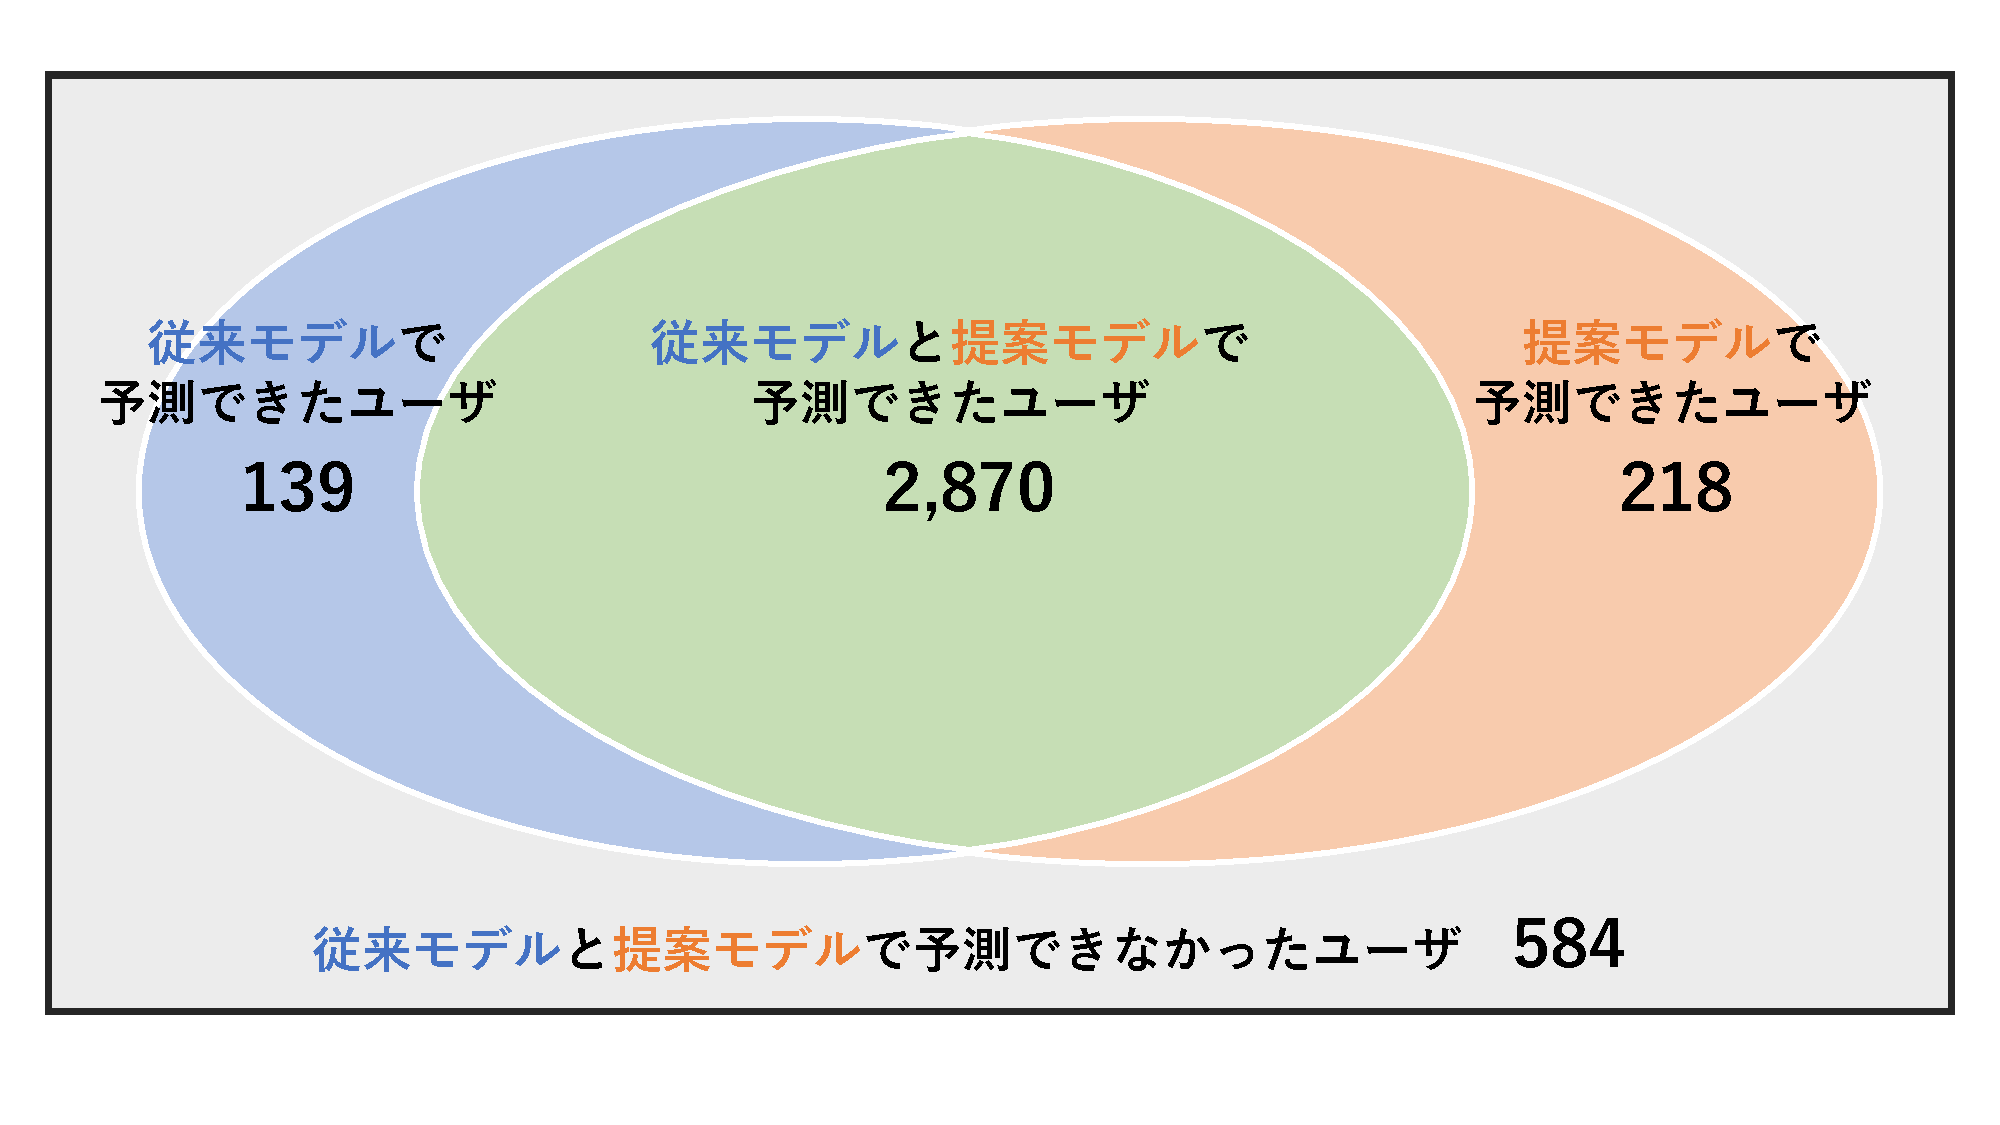
\includegraphics[width=1.0\linewidth]{Okamoto_fig/btod-venn.pdf}
%         %\vspace{-15mm}
% 	\caption{従来BtoDモデルと提案BtoDモデルで予測できたユーザと予測できなかったユーザ}
% 	\label{fig:btod-venn}
 
% 	\centering
% 	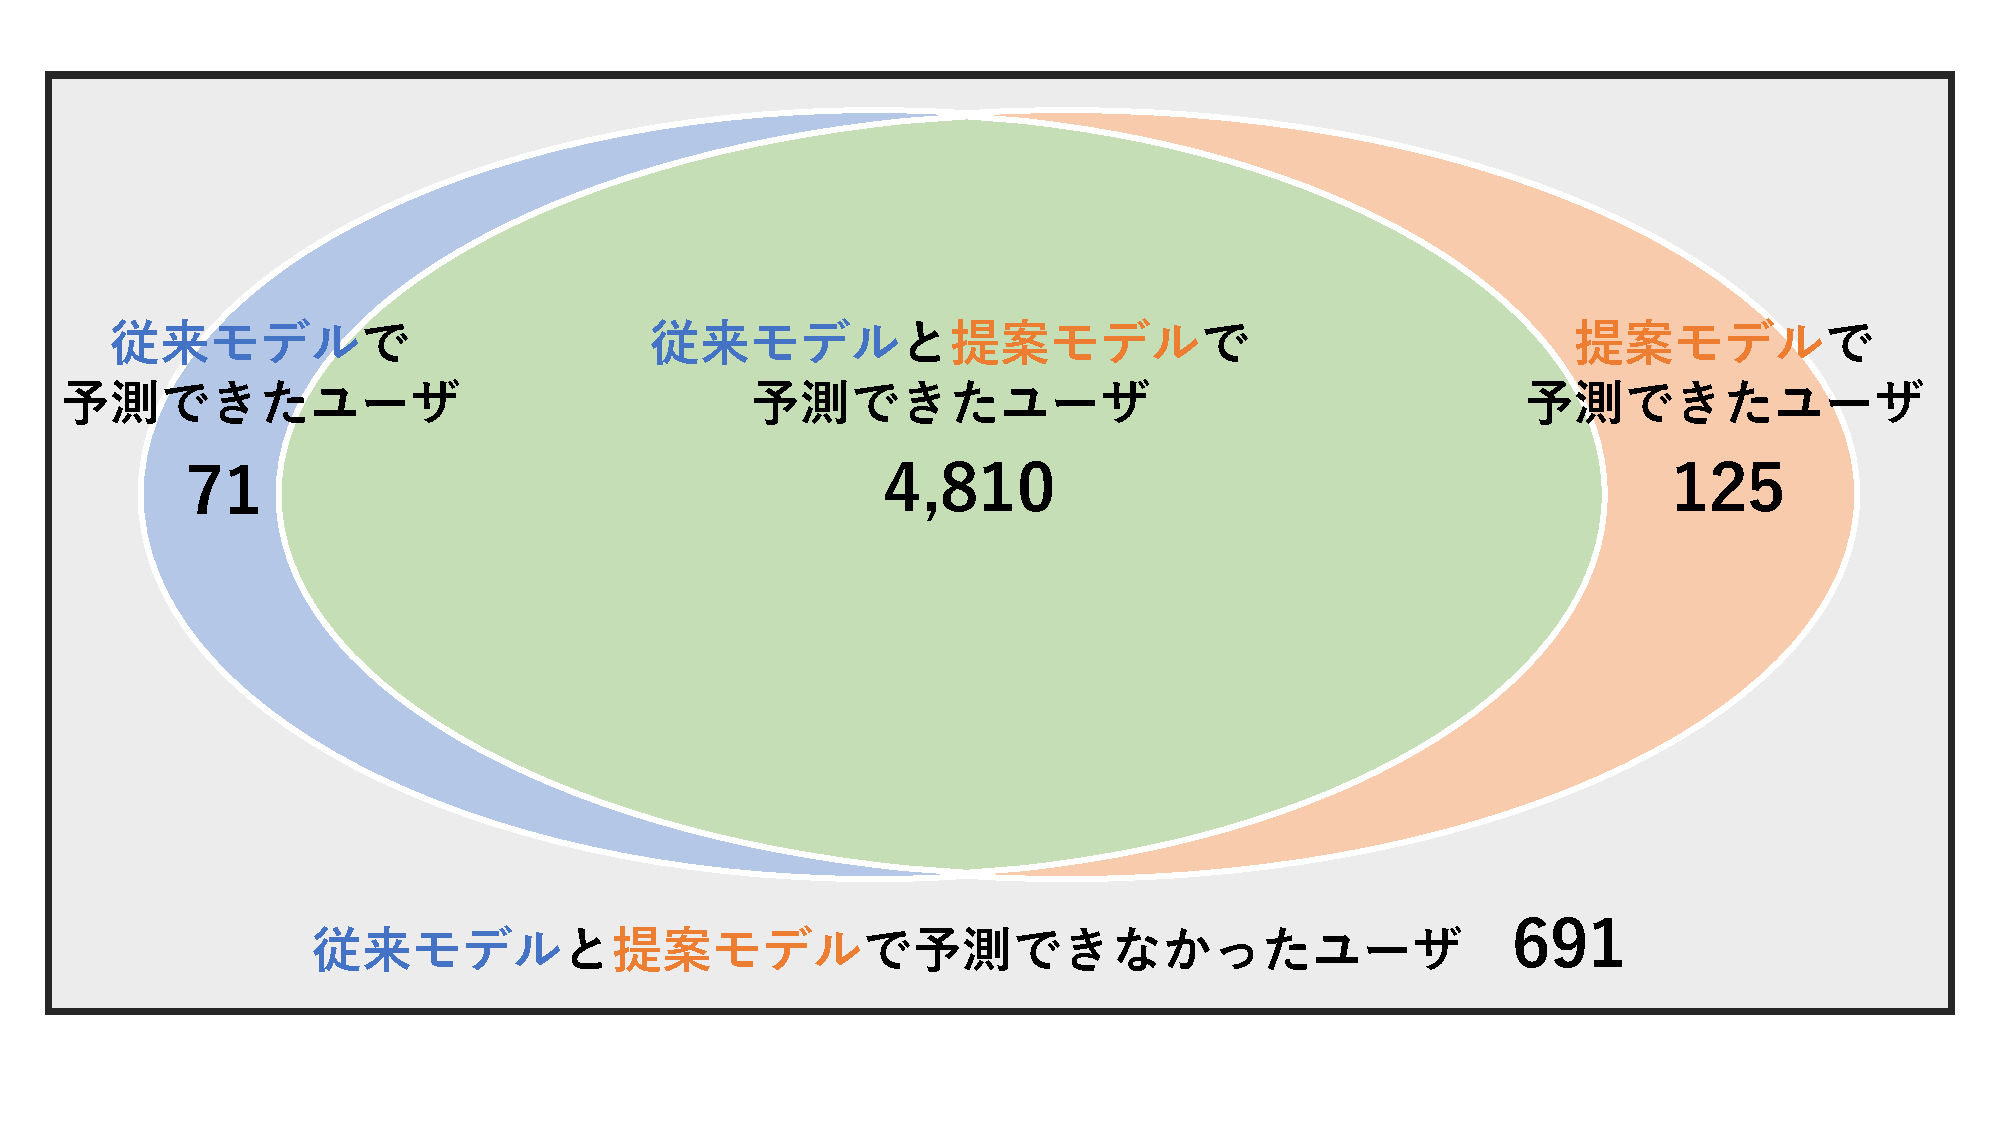
\includegraphics[width=1.0\linewidth]{Okamoto_fig/dtom-venn.pdf}
%         %\vspace{-15mm}
% 	\caption{従来DtoMモデルと提案DtoMモデルで予測できたユーザと予測できなかったユーザ}
% 	\label{fig:dtom-venn}
% \end{figure}

\begin{table}[t]
    \centering
    \caption{N階マルコフ連鎖モデルで予測が成功し,従来手法で誤予測したBtoDユーザの作品制作過程の事例}
    \ecaption{Actual example of produced work process for BtoD users that was successfully predicted using our proposed Markov chain model and incorrectly predicted using the previous model.}
    \label{tab:path-btod}
    \vspace{3mm}
    \scalebox{0.85}{
      \begin{tabular}{c|c|cccccccc}
\hline\hline
\multirow{2}{*}{制作順序} & \multicolumn{1}{l|}{\multirow{2}{*}{\small{リミックス}}} & \multicolumn{8}{c}{CTスコア}                                                                                                                                                         \\ \cline{3-10} 
                    & \multicolumn{1}{l|}{}                       & \multicolumn{1}{c|}{A} & \multicolumn{1}{c|}{P} & \multicolumn{1}{c|}{L} & \multicolumn{1}{c|}{S} & \multicolumn{1}{c|}{F} & \multicolumn{1}{c|}{U} & \multicolumn{1}{c|}{D} & 合計 \\ \hline 
1                   & 1                                           & \multicolumn{1}{c|}{1} & \multicolumn{1}{c|}{0} & \multicolumn{1}{c|}{0} & \multicolumn{1}{c|}{1} & \multicolumn{1}{c|}{1} & \multicolumn{1}{c|}{2} & \multicolumn{1}{c|}{1} & 6  \\ \hline
2                   & 0                                           & \multicolumn{1}{c|}{1} & \multicolumn{1}{c|}{1} & \multicolumn{1}{c|}{0} & \multicolumn{1}{c|}{1} & \multicolumn{1}{c|}{2} & \multicolumn{1}{c|}{1} & \multicolumn{1}{c|}{1} & 7  \\ \hline
3                   & 1                                           & \multicolumn{1}{c|}{1} & \multicolumn{1}{c|}{1} & \multicolumn{1}{c|}{0} & \multicolumn{1}{c|}{1} & \multicolumn{1}{c|}{2} & \multicolumn{1}{c|}{1} & \multicolumn{1}{c|}{1} & 7  \\ \hline
4                   & 0                                           & \multicolumn{1}{c|}{1} & \multicolumn{1}{c|}{1} & \multicolumn{1}{c|}{0} & \multicolumn{1}{c|}{1} & \multicolumn{1}{c|}{2} & \multicolumn{1}{c|}{1} & \multicolumn{1}{c|}{1} & 7  \\ \hline
5                   & 0                                           & \multicolumn{1}{c|}{1} & \multicolumn{1}{c|}{2} & \multicolumn{1}{c|}{0} & \multicolumn{1}{c|}{0} & \multicolumn{1}{c|}{1} & \multicolumn{1}{c|}{2} & \multicolumn{1}{c|}{1} & 7  \\ \hline
6                   & 0                                           & \multicolumn{1}{c|}{1} & \multicolumn{1}{c|}{1} & \multicolumn{1}{c|}{0} & \multicolumn{1}{c|}{1} & \multicolumn{1}{c|}{1} & \multicolumn{1}{c|}{1} & \multicolumn{1}{c|}{1} & 6  \\ \hline
7                   & 1                                           & \multicolumn{1}{c|}{1} & \multicolumn{1}{c|}{3} & \multicolumn{1}{c|}{0} & \multicolumn{1}{c|}{3} & \multicolumn{1}{c|}{2} & \multicolumn{1}{c|}{1} & \multicolumn{1}{c|}{1} & 11  \\ \hline
8                   & 0                                           & \multicolumn{1}{c|}{1} & \multicolumn{1}{c|}{3} & \multicolumn{1}{c|}{0} & \multicolumn{1}{c|}{3} & \multicolumn{1}{c|}{1} & \multicolumn{1}{c|}{1} & \multicolumn{1}{c|}{1} & 10  \\ \hline
\end{tabular}
}
  \end{table}

% %%%%%%%%%%%%%%%%%%%%%%%%%%
% \section{妥当性への脅威}\label{sec:limit}
% %%%%%%%%%%%%%%%%%%%%%%%%%%

% \noindent\textbf{内的妥当性: }本研究は,CTスキルの習熟過程がマルコフ過程に基づいていると仮定している.しかし,実際にはCTの習熟には他の要因も存在することが考えられる.しかし,従来研究\cite{Ando_2021}からもユーザは作品を繰り返す制作することで,CTスコアを向上させていることから,CTスキルの習熟過程はマルコフ過程に基づいていると仮定できると考える.

% \noindent\textbf{外的妥当性: }本研究は,ユーザが実際にScratch上に公開する作品を基に習熟度到達予測モデルを構築した.その際にオリジナル作品の判断はScratch APIを用いて取得して情報を用いて行ったが,ユーザが他者に支援してもらい制作した作品が存在することも考えられる.本研究ではユーザ6,323人が制作した作品126,460件を収集して,多くの作品データを分析対象とすることで脅威を軽減する.




%%%%%%%%%%%%%%%%%%%%%%%%%
%1
\section{RQ3:CTスキルの使用履歴の違いによって特定の習熟度に到達した作品のCTスコアは偏っているのか?}
\label{sec:rq3}
%%%%%%%%%%%%%%%%%%%%%%%%%

%RQ1では,習熟度の向上したユーザのうち,特定のCTスコアに到達したユーザを対象に,作品制作数毎にその過程で獲得してきたCT概念のパターンを明らかにした.
RQ2では,過去に制作した作品のCTパスが共通するユーザを対象に,特定の習熟度に到達するか否かを\textcolor{red}{\UnderlineTex{[変更1-3-25]予測するモデル}}を構築したが,N階連鎖マルコフモデルではCTパスが多様であることが原因で階数の増加に伴い予測できないユーザ数が増加した.CTパスが多様であれば,特定の習熟度到達時に制作するCTスキルも多様であることが示唆される.RQ3では,N階連鎖マルコフモデルで予測できないユーザが多い理由を定量的に明らかにするために,CTスキルの使用履歴の違いによって特定の習熟度に到達した作品のCTスコアの偏りを分析する.

\subsection{分析対象}
RQ2において,BtoDユーザが\textcolor{red}{\UnderlineTex{[変更1-3-5]Developing以上に到達}}する直前のCTパスは非BtoDユーザよりも重複数が多い事が明らかになった.さらにN階マルコフ連鎖モデルの結果から,モデルに学習させるパスの長さが3を超えると半数以上のユーザが予測できないことが明らかとなった.\textcolor{red}{\UnderlineTex{[変更1-3-26]これらの結果から}}\textcolor{red}{\UnderlineTex{[変更1-3-5]Developing以上に到達}}する直前に制作した作品は,Masterに到達する直前に制作した作品に比べて共通したCTスコアを使用していることが示唆される.そのため,本章ではBtoDユーザを対象に2作品目または3作品目に\textcolor{red}{\UnderlineTex{[変更1-3-5]Developing以上に到達}}する作品を制作したユーザのCTパスを分析する.
%また,RQ1の考察より,DtoMユーザがMasterに到達する直前のCTパスは非BtoDユーザよりも重複数が少ない事が明らかになった.この結果はMasterに到達する直近にはDtoMユーザは多様なCTスコアを獲得していることを示しており,本分析の対象とするパスの共通するユーザを抽出するのが困難であるため,本章においてDtoMユーザは分析の対象外とする.

% 本分析では習熟度向上の際のCTスコアの多様性を調査するため,対象ユーザが習熟度向上の際に制作した作品のCTスコアも含めたCTパスの重複数を算出する.

% \todo{分析手法}

\subsection{結果と考察}

\begin{table}[t]
  \caption{2番目または3番目にDevelopingの作品を制作したBtoDユーザ数,およびDevelopingを制作するまで(\textcolor{red}{\UnderlineTex{[変更1-3-5]Developing以上に到達}}時の作品を含む)のCTパスの種類数}
  \ecaption{Number of BtoD users who produced Developing level work on a 2nd or 3rd, and the number of the CT path types.}
  \label{tab:ct-users}
  \vspace{2mm}
  \centering
  \scalebox{0.9}{
  \begin{tabular}{c|c|c}
    \hline\hline
    作品制作数 & BtoDユーザ数 & 習熟度向上作品の\textcolor{red}{\UnderlineTex{CTパス種類数}}\\
    \hline
    2 & 694 & 523\\
    \hline
    3 & 423 & 384\\
    \hline
  \end{tabular}
    }
   \vspace{-2mm}
\end{table}


\begin{table}[t]
  \caption{2作品目または3作品目にDevelopingの作品を制作したユーザのCTパス重複数とそのパターン数}
  \ecaption{Number of CT path overlapping CT paths and their patterns for users who produced a 2nd or 3rd work.}
  \label{tab:goal-pattern-2}
  \centering
  \scalebox{0.87}{
  \begin{tabular}{c|c|c||c|c|c}
    \cline{1-3}\cline{4-6}
    \multicolumn{3}{c||}{\textcolor{red}{\UnderlineTex{2作品目}}} & \multicolumn{3}{c}{\textcolor{red}{\UnderlineTex{3作品目}}} \\
    \cline{1-3}\cline{4-6}
    順位 & パス重複数 & パターン数 & 順位 & パス重複数 & パターン数 \\
    \cline{1-3}\cline{4-6}
    1 & 18 & 1 & 1 & 5 & 2 \\
    \cline{1-3}\cline{4-6}
    2 & 11 & 1 & 2 & 4 & 2 \\
    \cline{1-3}\cline{4-6}
    3 & 9 & 1 & 3 & 3 & 2 \\
    \cline{1-3}\cline{4-6}
    4 & 8 & 1 & 4 & 2 & 10 \\
    \cline{1-3}\cline{4-6}
  \end{tabular}
  }
   \vspace{-2mm}
\end{table}

表\ref{tab:ct-users}は,\textcolor{red}{\UnderlineTex{[変更1-3-28]2番目または3番目に}}Developingの作品を制作したBtoDユーザ数,およびDevelopingを制作するまで(\textcolor{red}{\UnderlineTex{[変更1-3-5]Developing以上に到達}}時の作品を含む)のCTパスの種類数を示す.\textcolor{red}{\UnderlineTex{[変更1-2-6]表16}}
%\ref{tab:ct-users}
から,2番目または3番目にDevelopingの作品を制作したBtoDユーザがそれぞれ694人,423人存在し,各ユーザが制作したCTパスの種類数は523種類と384種類であるため,ユーザはDevelopingの作品を制作する際に多様なCTスコアを獲得している.
%作品制作数2または3のBtoDユーザが初めて習熟度が向上した際に制作した作品(習熟度向上作品)のCTスコアの種類数を示す.

次に,CTスキルの使用履歴の違いによるCTスコアの多様性を明らかにするために,\textcolor{red}{\UnderlineTex{[変更1-3-5]Developing以上に到達}}時に共通のCTスコアを制作したユーザのCTパス(\textcolor{red}{\UnderlineTex{[変更1-3-5]Developing以上に到達}}時の作品を含まない)重複数とそのパターン数を示す.表\ref{tab:goal-pattern-2}は,\textcolor{red}{\UnderlineTex{[変更1-3-29]2作品目または3作品目に}}Developingの作品を制作したユーザのCTパス重複数とそのパターン数の上位4件を示す.\textcolor{red}{\UnderlineTex{[変更1-2-8][変更C2-3]表14}}
%\ref{tab:goal-pattern-2}
から,2作品目または3作品目で\textcolor{red}{\UnderlineTex{[変更1-3-5]Developing以上に到達}}したユーザの重複数の最大値は18であり,\textcolor{red}{\UnderlineTex{[変更1-2-9]2}}作品目で\textcolor{red}{\UnderlineTex{[変更1-3-5]Developing以上に到達}}したユーザの重複数の最大値はそれぞれ18,5であり,表\ref{tab:ct-users}に比べると\textcolor{red}{\UnderlineTex{[変更1-3-5]Developing以上に到達}}する直前の作品のCTスコアは共通しているが,重複数が多いとは言い難い.したがって,DtoMユーザに比べてBtoDユーザの方が過去に制作する作品のCTスコアが共通しているが,CTパスが多様であるためRQ2で予測できないユーザを多数確認した.今後はN階マルコフモデルにおいて\textcolor{red}{\UnderlineTex{[変更1-3-5]Developing以上に到達}}した作品のCTスコアの類似性に着目することで,習熟度到達予測の精度改善が期待される.

%%%%%%%%%%%%%%%%%%%%%%%%%%
\section{おわりに}\label{sec:conc}
%%%%%%%%%%%%%%%%%%%%%%%%%%

本研究では,特定の習熟度に到達するまでの過程で使用したCTスキル,および各CTスキルを用いたユーザの作品制作数を分析し,習熟度を予測するモデルを構築した.提案するモデルは従来手法よりも高い精度でユーザの習熟度を予測できることを確認した.今後は,マルコフ連鎖モデルの汎用性を高める方法を検討し,ScratchにおけるユーザのCTスキル獲得状況に合わせた作品推薦に取り組む.


% 参考文献
%\bibliographystyle{ipsjunsrt}
%\bibliography{bibfile}
\bibliographystyle{junsrt}
\bibliography{Okamoto}

% 著者一覧
\begin{biography}
\profile{s}{岡本 圭悟}{2020年和歌山大学システム工学部卒業.現在,同大学同学部博士前期課程に在学中.ソフトウェア工学,特にプログラミング学習支援の研究に従事.}
%
\profile{m}{伊原 彰紀}{2007年龍谷大学理工学部卒業.2009年奈良先端科学技術大学院大学情報科学研究科博士前期課程修了.2012年同大学博士後期課程修了.2012年同大学情報科学研究科助教.2018年和歌山大学システム工学部講師.博士(工学).ソフトウェア工学,特にオープンソースソフトウェア開発・利用支援の研究に従事.電子情報通信学会,ソフトウェア科学会,IEEE各会員.}
\end{biography}

\end{document}